\chapter{Categories, Functors and Natural Transformations.} 
    \section{Introduction: What are the Foundations of Math?} 
    Category theory attempts to ``zoom out'' of mathematical constructions
    and to point out the higher level relationships between different mathematical
    constructions. The three main concepts are categories, functors, and
    natural transformations, although the theory grew out of
    implications of these main concepts. 
    
    
    These main concepts were first seen in the study of algebraic
    topology, since 
    it was observed that topological problems could be reduced to
    algebraic, and vice versa. But how? Since there was no formal
    notion for what it really meant to take a topological space $X$
    and associate it with some group $\pi(X)$, 
    category theory came about to formalize this. 

    However, as we shall soon see, category theory has a big problem. 
    Specifically, there isn't a universally agreed upon foundation for
    category theory, or for mathematics in general. 
    \begin{center}
        \textbf{What do we mean by foundations?}
    \end{center}
    Well, consider a topological space $X$, or a group $G$, or a
    domain $\mathbb{R}$. Then suppose I ask you
    ``What is $X$?'' or ``What is $G$'' or ``What is $\mathbb{R}$?'' 
    Well, you'll tell me it's a topological space, a
    group, or the set of real numbers and
    list the axioms for each object. 

    That is, a correct answer will characterize $X$, $G$ or $\mathbb{R}$ as a
    set which satisfies 
    some axioms. But really, that's what all our mathematical objects
    are. So at this point, our foundations \textbf{are grounded in set
    theory.}

    \begin{center}
        \textbf{What is set theory?}
    \end{center}
    Suppose I ask you what is set theory. While we all know there are 
    different set theories, most people don't think about set theory axioms on a daily 
    and won't know (like myself). But answering
    this question requires answering the next. 

    \begin{center}
    \textbf{What is a set?}
    \end{center}
    We usually never have to face this question. But in developing a
    theory that considers relationships between different sets, we
    have to. 
    
    Our intuition tells us that sets $X$ are a \textbf{collection of
    objects, and that every collection of objects is a set}. We
    intuitively \textit{think} that  
    we can form collections of objects to create a set $X$, and that
    we can form 
    intersection and unions between sets, or even compute power
    sets, to produce other sets. We also \textit{think} we can also form sets such as 
    \[
        X = \{x \mid \phi(x) \}
    \]
    where $\phi$ is some logical condition of inclusion. However, this
    leads to paradoxes, one of the most famous known as Russel's
    Paradox which we can describe as follows. 

    \noindent\textbf{Russel's Paradox.}
    Let $X$ be a set such that 
    \[
        X = \{A \text{ is a set }\mid A \text{ is not a member of itself.}\}
    \]
    
    Now observe the following. 
    \begin{itemize}
        \item[1.] If $X \in X$, then consequently $X$ is not a member
        of itself. In other words, if $X \in X$, then $X \not\in X$.

        Clearly, this is a contradiction. Since $X \in X$ is nonsense,
        $X \not\in X$, right? 

        \item[2.] Suppose $X \not\in X$. Then $X$ is not a member of
        itself, so $X \in X$ by the condition of member of $X$. In
        other words, $X \not\in X \implies X \in X$.
    \end{itemize}
    See the problem here? \textbf{Not every collection of objects is a
    set.} So our previous notions of sets aren't correct.

    \textcolor{MidnightBlue}{Note that our trouble arose when we said
    that \textbf{a set is a collection of objects, and a collection of
    objects is a set.} 
    This is because no, not every collection of objects is a set.
    Thus we need to go back and fix our definition of a set.
    }

    \begin{center}
        \textbf{What do we do?}
    \end{center}
    This is what many mathematicians asked in the early 1900s
    when they identified the paradoxes that arise from our notion of
    a set. The result has been multiple different types of set theories, 
    and so there isn't a clear 
    choice on what to make our foundations. However, this isn't a huge problem 
    for category theory. Category theory 
    has its own core axioms, but the fact that there are different set theories 
    simply means that such core axioms will be phrased differently under different 
    set theories (although there are some cases where 
    one does need to be careful with their foundations).
    In this text, we'll be a bit sloppy with the foundations of category theory, 
    although  we will point out where we need to be careful.


    \newpage
    \section{Motivation for Category Theory}
    What do groups $G$, topological spaces $X$ and vector spaces $V$ have 
    in common?
    \emph{We use different letters to describe them!} Seriously, that is one major 
    difference. Why? Because our brains are organizational and thrive off of associations, 
    e.g., $G$ with group, $X$ with topological spaces, etc. This is great 
    for thinking, but the mental separation of these constructions hides a bigger 
    picture.

    Let's look at what these things look like. 
    With groups, we are often mapping between groups via group homomorphisms.
    For example, below we have the chain complex of abelian groups with boundary 
    operator $\partial_n: C_n \to C_{n-1}$, with the familiar property that
    $\partial_n \circ \partial_{n-1} = 0$.
    \begin{center}
    \adjustbox{scale = 0.85}{
        \tikzstyle{A} = [fill=ProcessBlue!20]
        \tikzstyle{B} = [fill=ProcessBlue!30]
        \tikzstyle{C} = [fill=ProcessBlue!40]
        \begin{tikzpicture}[>=stealth]
            \pgfmathsetmacro{\height}{2.5}
            \pgfmathsetmacro{\heightstep}{0.5}
            \pgfmathsetmacro{\width}{2}
            \pgfmathsetmacro{\widthstep}{0.5}
            
            \pgfmathsetmacro{\Ax}{\height}
            \pgfmathsetmacro{\Ay}{\width}
            \pgfmathsetmacro{\Bx}{\height - \heightstep}
            \pgfmathsetmacro{\By}{\width - \widthstep}
            \pgfmathsetmacro{\Cx}{\height - \heightstep -\heightstep}
            \pgfmathsetmacro{\Cy}{\width - \widthstep - \widthstep}
    
            \begin{scope}
                % draws the three ellipses
                \filldraw[A] (0,0) ellipse (\Ay cm and \Ax cm);
                \draw (0,0) ellipse (\Ay cm and \Ax cm);
    
                \filldraw[B] (0,-\heightstep) ellipse (\By cm and \Bx cm);
                \draw (0,-\heightstep) ellipse (\By cm and \Bx cm);
    
                \filldraw[C] (0,-\heightstep - \heightstep) ellipse (\Cy cm and \Cx cm);
                \draw (0,-\heightstep - \heightstep) ellipse (\Cy cm and \Cx cm);
    
                % labels the ellipses
                \node at (0, \height - 0.3) {$C_n$};
                \node at (0, \height - 1.3) {$Z_n$};
                \node at (0, \height - 2.4) {$B_n$};
            \end{scope}
    
            \begin{scope}[xshift = 5cm]
                % draws the three ellipses
                \filldraw[A] (0,0) ellipse (\Ay cm and \Ax cm);
                \draw (0,0) ellipse (\Ay cm and \Ax cm);
        
                \filldraw[B] (0,-\heightstep) ellipse (\By cm and \Bx cm);
                \draw (0,-\heightstep) ellipse (\By cm and \Bx cm);
        
                \filldraw[C] (0,-\heightstep - \heightstep) ellipse (\Cy cm and \Cx cm);
                \draw (0,-\heightstep - \heightstep) ellipse (\Cy cm and \Cx cm);
    
                % labels the ellipses
                \node at (0, \height - 0.3) {$C_{n-1}$};
                \node at (0, \height - 1.3) {$Z_{n-1}$};
                \node at (0, \height - 2.4) {$B_{n-1}$};
            \end{scope}
    
            \begin{scope}[xshift = 10cm]
                % draws the three ellipses
                \filldraw[A] (0,0) ellipse (\Ay cm and \Ax cm);
                \draw (0,0) ellipse (\Ay cm and \Ax cm);
        
                \filldraw[B] (0,-\heightstep) ellipse (\By cm and \Bx cm);
                \draw (0,-\heightstep) ellipse (\By cm and \Bx cm);
        
                \filldraw[C] (0,-\heightstep - \heightstep) ellipse (\Cy cm and \Cx cm);
                \draw (0,-\heightstep - \heightstep) ellipse (\Cy cm and \Cx cm);
    
                % labels the ellipses
                \node at (0, \height - 0.3) {$C_{n-2}$};
                \node at (0, \height - 1.3) {$Z_{n-2}$};
                \node at (0, \height - 2.4) {$B_{n-2}$};
            \end{scope}
    
            % draws the arrows
            \draw[->] (0.5, \height-0.5) -- (4.2cm, \height-2.5) node[midway, above] {$\partial_n$};
            \draw[->] (0.5+5.5cm, \height-0.5) -- (4.2cm+5cm, \height-2.5) node[midway, above] {$\partial_{n-1}$};
    
            \draw[->] (0.2, \height-1.6) -- (4.8, -2.3)node[midway, below] {$\partial_n$};
            \draw[->] (0.2+5.5cm, \height-1.6) -- (9.7cm, -2.3)node[midway, below] {$\partial_{n-1}$};
    
            \filldraw (0,-2.5) circle (0.5mm) node[below] {$0$};
            \filldraw (5cm,-2.5) circle (0.5mm) node[below] {$0$};
            \filldraw (10cm,-2.5) circle (0.5mm) node[below] {$0$};
    
            \node at (-3cm, 0cm) {$\cdots$};
            \node at (13cm, 0cm) {$\cdots$};
        \end{tikzpicture}
    }

    \emph{A chain complex; the image of $\partial_n$ is $B_{n-1}$, while the kernel 
    of $\partial_n$ is $Z_{n}$.}
    \end{center}

    Within topology, we are often mapping topological spaces via continuous functions.
    \begin{center}
        % controls surface color
        \tikzstyle{surface}=[left color=NavyBlue!30,right color=NavyBlue!60, 
        opacity = 0.8
        ]
        % controls the embedded triangle surface color
        \tikzstyle{em_triangle}=[left color=Purple!30,right color=Purple!60,
        opacity = 0.8
        ]
        % controls the triangle surface color
        \tikzstyle{triangle}=[left color=Purple!30,right color=Purple!50,
        opacity = 0.8
        ]
        % controls the shadow coloring
        \tikzstyle{shadow}=[left color=gray!10,right color=gray!20, opacity = 0.8, rounded corners=0.5cm]
    
        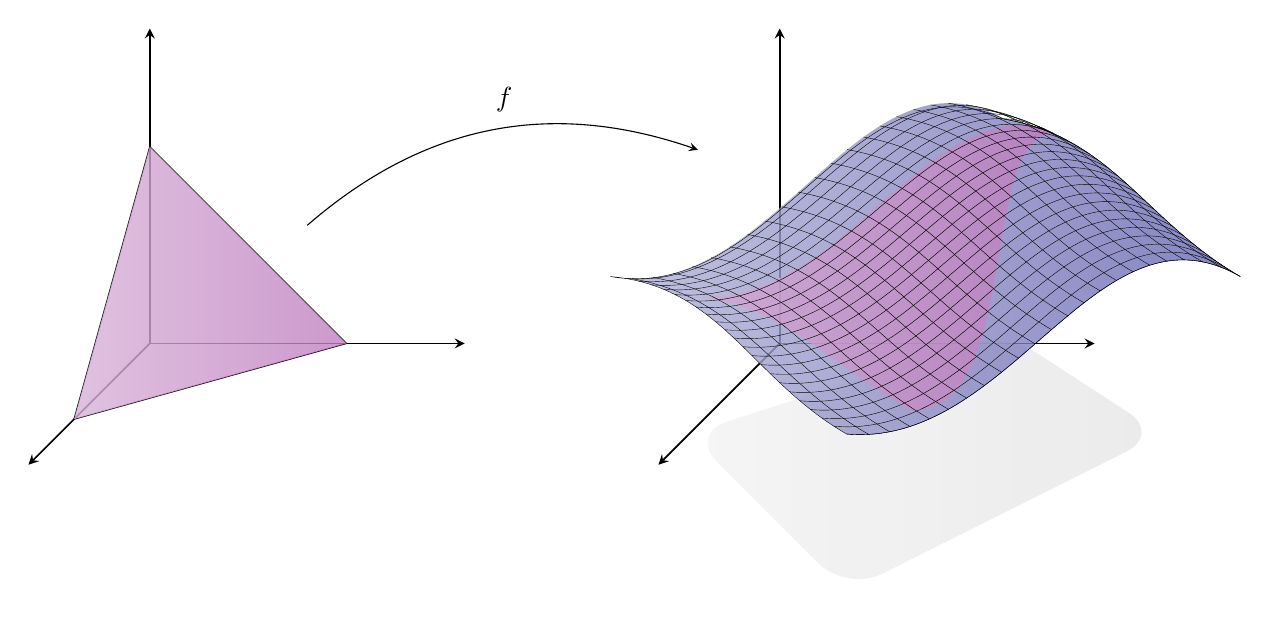
\begin{tikzpicture}[>=stealth]
            \pgfmathsetmacro{\scale}{4}
            \pgfmathsetmacro{\zoffset}{-10}
            \pgfmathsetmacro{\yoffset}{-3}
            \pgfmathsetmacro{\xoffset}{-6}
        
            % the origin
            \coordinate (origin) at (-\xoffset, -\yoffset, -\zoffset);
        
            % the axes
            \coordinate (A) at (\scale -\xoffset, -\yoffset,-\zoffset);
            \coordinate (B) at (-\xoffset, \scale-\yoffset,-\zoffset);
            \coordinate (C) at (-\xoffset, -\yoffset,\scale-\zoffset);
        
            \draw[semithick, ->] (origin) --  (A);
            \draw[semithick, ->] (origin) --  (B);
            \draw[semithick, ->] (origin) --  (C);
    
            % the leftmost axes 
            \pgfmathsetmacro{\axesshift}{8}
            \coordinate (a) at (\scale -\xoffset - \axesshift, -\yoffset,-\zoffset);
            \coordinate (b) at (-\xoffset -  \axesshift, \scale-\yoffset,-\zoffset);
            \coordinate (c) at (-\xoffset - \axesshift, -\yoffset,\scale-\zoffset);
            
            % the leftmost origin
            \coordinate (left_origin) at (-\xoffset - \axesshift, -\yoffset, -\zoffset);
            \draw[semithick, ->] (left_origin) --  (a);
            \draw[semithick, ->] (left_origin) --  (b);
            \draw[semithick, ->] (left_origin) --  (c);
    
            % triangle
            \pgfmathsetmacro{\trianglelength}{2.5}
    
            % boundary of triangle
            \draw (\trianglelength-\xoffset - \axesshift,-\yoffset,-\zoffset) 
            -- 
            (-\xoffset -\axesshift, \trianglelength-\yoffset, -\zoffset) 
            -- 
            (-\xoffset -\axesshift, -\yoffset, \trianglelength-\zoffset) -- cycle;
    
            % interior of triangle
            \shade[triangle]
            (\trianglelength-\xoffset - \axesshift,-\yoffset,-\zoffset) 
            -- 
            (-\xoffset -\axesshift, \trianglelength-\yoffset, -\zoffset) 
            -- 
            (-\xoffset -\axesshift, -\yoffset, \trianglelength-\zoffset) -- cycle;
    
            
            % the arrow
            \draw[->] ([xshift = -2cm, yshift = 1.5cm]a) 
            to[bend left] 
            ([xshift= 0.5cm, yshift = 4cm]C);
            \node at ([xshift = 0.5cm, yshift = 3.1cm]a) {$f$};
    
            % number of lines (n x n grid)
            \pgfmathsetmacro{\nlines}{22}
            % coordinates
            \coordinate (A) at (0,0);
            \path (A);\pgfgetlastxy{\ax}{\ay} 
            \coordinate (B) at (3,-2);
            \path (B);\pgfgetlastxy{\bx}{\by}
            \coordinate (C) at (8,0);
            \path (C);\pgfgetlastxy{\cx}{\cy}
            \coordinate (D) at (5, 2);
            \path (D);\pgfgetlastxy{\dx}{\dy}
        
            %incoming angles
            \pgfmathsetmacro{\ABout}{-5}
            \pgfmathsetmacro{\ABin}{150}
            
            \pgfmathsetmacro{\BCout}{-5}
            \pgfmathsetmacro{\BCin}{150}
        
            \pgfmathsetmacro{\CDout}{150}
            \pgfmathsetmacro{\CDin}{-10}
            
            \pgfmathsetmacro{\DAout}{150}
            \pgfmathsetmacro{\DAin}{-10}
        
            % draws the shadow underneath
            \shade[shadow]
            ([xshift = 1cm, yshift = -2cm]A)
            --
            ([xshift = 0cm, yshift = -2cm]B) 
            --
            ([xshift = -1cm, yshift = -2cm]C)
            --
            ([xshift = 0cm, yshift = -2.7cm]D) 
            --
            % to[out=\DAout,in=\DAin]  
            cycle;
        
            % draws the colored surface 
            \shade[surface] 
            (A)
            to[out=\ABout,in=\ABin] 
            (B) 
            to[out=\BCout,in=\BCin] 
            (C)
            to[out=\CDout,in=\CDin] 
            (D) 
            to[out=\DAout,in=\DAin]  cycle;
        
            % draws the thin boundary
            \draw[line width = 0.05mm]
            (A)
            to[out=\ABout,in=\ABin] 
            (B) 
            to[out=\BCout,in=\BCin] 
            (C)
            to[out=\CDout,in=\CDin] 
            (D) to[out=155,in=\DAin] cycle;
        
            % draws the vertical grid lines
            \foreach \n in {1,2, ..., \nlines}{
                \pgfmathsetmacro{\step}{\n/\nlines}
                \path (A) to[out=\ABout,in=\ABin] coordinate[pos=\step] (A\n) (B);
                \path (B) to[out=\BCout,in=\BCin] coordinate[pos=\step] (B\n) (C);
                \path (D) to[in=\CDout,out=\CDin] coordinate[pos=\step] (C\n) (C);
                \path (A) to[in=\DAout,out=\DAin] coordinate[pos=\step] (D\n) (D);
            }
        
            % draws the horizontal grid lines
            \foreach \n in {1,2,...,\nlines}{
                \path (A\n); \pgfgetlastxy{\ax\n}{\ay\n} 
                \path (B\n); \pgfgetlastxy{\bx\n}{\by\n} 
                \path (C\n); \pgfgetlastxy{\cx\n}{\cy\n} 
                \path (D\n); \pgfgetlastxy{\dx\n}{\dy\n} 
                \draw[line width = 0.05mm]
                (\bx\n,\by\n) to[out=\DAout,in=\DAin] (\dx\n,\dy\n);
                \draw[line width = 0.05mm]
                (\ax\n,\ay\n) to[out=\ABout,in=\ABin] (\cx\n,\cy\n);
            }
        
            % draws the embedded triangular surface.
            \begin{scope}
                % embedded triangle outline
                \clip ([xshift = 0.1cm]A5)
                to[out=\ABout,in=\ABin] 
                ([xshift = -0.5cm]B5) 
                to[out=\BCout,in=\BCin] 
                ([xshift = 0.1cm]C5)
                to[out=\CDout,in=\CDin] 
                cycle;
    
                % number of lines (n x n grid)
                \pgfmathsetmacro{\nlines}{22}
                % coordinates
                \coordinate (A) at (0,0);
                \path (A);\pgfgetlastxy{\ax}{\ay} 
                \coordinate (B) at (3,-2);
                \path (B);\pgfgetlastxy{\bx}{\by}
                \coordinate (C) at (8,0);
                \path (C);\pgfgetlastxy{\cx}{\cy}
                \coordinate (D) at (5, 2);
                \path (D);\pgfgetlastxy{\dx}{\dy}
            
                %incoming angles
                \pgfmathsetmacro{\ABout}{-5}
                \pgfmathsetmacro{\ABin}{150}
                
                \pgfmathsetmacro{\BCout}{-5}
                \pgfmathsetmacro{\BCin}{150}
            
                \pgfmathsetmacro{\CDout}{150}
                \pgfmathsetmacro{\CDin}{-10}
                
                \pgfmathsetmacro{\DAout}{150}
                \pgfmathsetmacro{\DAin}{-10}
            
                % draws the colored surface 
                \shade[em_triangle] 
                (A)
                to[out=\ABout,in=\ABin] 
                (B) 
                to[out=\BCout,in=\BCin] 
                (C)
                to[out=\CDout,in=\CDin] 
                (D) 
                to[out=\DAout,in=\DAin]  cycle;
            
                % draws the thin boundary
                \draw[line width = 0.05mm]
                (A)
                to[out=\ABout,in=\ABin] 
                (B) 
                to[out=\BCout,in=\BCin] 
                (C)
                to[out=\CDout,in=\CDin] 
                (D) to[out=\DAout,in=\DAin] cycle;
            
                % draws the vertical grid lines
                \foreach \n in {1,2, ..., \nlines}{
                    \pgfmathsetmacro{\step}{\n/\nlines}
                    \path (A) to[out=\ABout,in=\ABin] coordinate[pos=\step] (A\n) (B);
                    \path (B) to[out=\BCout,in=\BCin] coordinate[pos=\step] (B\n) (C);
                    \path (D) to[in=\CDout,out=\CDin] coordinate[pos=\step] (C\n) (C);
                    \path (A) to[in=\DAout,out=\DAin] coordinate[pos=\step] (D\n) (D);
                }
            
                % draws the horizontal grid lines
                \foreach \n in {1,2,...,\nlines}{
                    \path (A\n); \pgfgetlastxy{\ax\n}{\ay\n} 
                    \path (B\n); \pgfgetlastxy{\bx\n}{\by\n} 
                    \path (C\n); \pgfgetlastxy{\cx\n}{\cy\n} 
                    \path (D\n); \pgfgetlastxy{\dx\n}{\dy\n} 
                    \draw[line width = 0.05mm]
                    (\bx\n,\by\n) to[out=\DAout,in=\DAin] (\dx\n,\dy\n);
                    \draw[line width = 0.05mm]
                    (\ax\n,\ay\n) to[out=\ABout,in=\ABin] (\cx\n,\cy\n);
                }
        
            \end{scope}
        \end{tikzpicture}

        \emph{A 2-simplex gets embedded into a manifold in $\rr^3$.}
    \end{center}
    
    With vector spaces, we often use linear transformations to map 
    from one to another. 
    \begin{center}
        \begin{tikzpicture}[>=stealth]
            % main arrow
            \draw[->] (-6,2) to[bend left] (-2,2);
            \node at (-2.5,3.2) {$T = \begin{pmatrix}
                2 & 0 \\
                1 & 2\\
                1 & 1
            \end{pmatrix}$};
    
            \begin{scope}[xshift = -8cm]
                % parameters
                \pgfmathsetmacro{\scale}{2.5}
                \coordinate (origin) at (0,0);
    
                % the axes
                \coordinate (A1) at (\scale, 0);
                \coordinate (A2) at (-\scale, 0);
                \coordinate (B1) at (0, \scale);
                \coordinate (B2) at (0, -\scale);
    
                \draw[semithick, ->] (origin) -- (A1) node[right] {$x$};
                \draw[semithick, ->] (origin) -- (B1) node[above] {$y$};
    
                \draw[semithick, ->] (origin) -- (A2) node[left] {$-x$};
                \draw[semithick, ->] (origin) -- (B2) node[below] {$-y$};
    
                \foreach \n/\col in {(1,2)/red, 
                (-1, 1)/green, 
                (-2, -1)/blue, 
                (0.5, -2)/orange, 
                (2, 1)/Purple}{
                    \draw[->, \col] (origin) --  \n;
                }
    
    
            \end{scope}
            \tdplotsetmaincoords{60}{110}
            \begin{scope}[tdplot_main_coords]
                % this takes in a 3x2 matrix, 2-vectors, and plots their 
                % image after evaluation with the matrix.
    
                % axes
                \pgfmathsetmacro{\scale}{5} % axes length
                \coordinate (O) at (0, 0, 0);         % origin
                \coordinate (Y) at (0, \scale-1, 0);    % y axes
                \coordinate (Z) at (0, 0, \scale-2);  % z axes
                \coordinate (X) at (\scale, 0, 0);    % x axes
                \coordinate (nY) at (0, -\scale+1, 0);   % -y axes
                \coordinate (nZ) at (0, 0, -\scale+2); % z axes
                \coordinate (nX) at (-\scale, 0, 0);   % x axes
    
                % axes labels
                \draw[semithick, ->] (O) -- (Y) node[right] {$y$};
                \draw[semithick, ->] (O) -- (Z) node[above] {$z$};
                \draw[semithick, ->] (O) -- (X) node[below] {$x$};
    
                \draw[semithick, ->] (O) -- (nY) node[above=1pt] {$-y$};
                \draw[semithick, ->] (O) -- (nZ) node[below] {$-z$};
                \draw[semithick, ->] (O) -- (nX) node[above] {$-x$};
                
                % the matrix
                \pgfmathsetmacro{\Aaa}{2}
                \pgfmathsetmacro{\Aab}{0}
                \pgfmathsetmacro{\Baa}{1}
                \pgfmathsetmacro{\Bab}{2}
                \pgfmathsetmacro{\Caa}{1}
                \pgfmathsetmacro{\Cab}{1}
    
                %%%%%%%%%%%%%% plotting 3D points %%%%%%%%%%%%%
                % input your (x,y) points as x/y
                \foreach \x/\y/\col in {1/2/red,
                2/-1/Green, 
                -2/1/Blue, 
                0.5/-2/orange,
                 2/1/Purple}
                {
                    \pgfmathsetmacro{\mx}{\x *\Aaa + \y *\Aab}
                    \pgfmathsetmacro{\my}{\x *\Baa + \y *\Bab}
                    \pgfmathsetmacro{\mz}{\x *\Caa + \y *\Cab}
                    \coordinate (M) at (\mx, \my, \mz);
    
                    \draw[\col, dashed] (M) -- (\mx, \my, 0);
                    \draw[\col, dashed] (\mx, \my, 0) -- (\mx, 0, 0);
                    \draw[\col, dashed] (\mx, \my, 0) -- (0, \my, 0);
    
                    % first point vector
                    \draw[\col, -latex] (O) -- (M) ;
                }
            \end{scope}
        \end{tikzpicture}
        \emph{Above we have $T: \rr^2 \to \rr^3$ as a linear transformation 
        sending the various colored vectors in $\rr^2$ to the vectors in $\rr^3$.
        The linear transformation itself is given above.
        }
    \end{center}
    At some point when we're learning different basic constructions in 
    pure mathematics, we often realize that we're just 
    repeating the same story over and over. The professor tells you about 
    an object (usually a set) equipped with some axioms. The next thing you learn 
    are ``mappings'' between such objects, which can abstractly be called \emph{morphisms}.
    The characteristics of these morphism
    are generally the following:
    \begin{description}
        \item[1.] There's an identity morphism.
        \item[2.] There's a notion of composition. 
        \item[3.] Composition is associative. 
        \item[4.] Composing identities in any order with a morphism 
        returns the same morphism. 
    \end{description}

    What is it that I just described? It sounds just like 
    a \emph{monoid}! In the most 
    basic sense, a monoid $M = \{x_1, x_2, \dots, \}$ is a set of elements equipped with 
    a multiplication map 
    \[
        \cdot: M \times M \to M \qquad (x, y) \mapsto x\cdot y
    \]
    which is associative, and with a multiplicative identity $e$. With a monoid we see that 
    \begin{description}
        \item[1.] There's an identity $e$.
        \item[2.] There's a notion of multiplication.
        \item[3.] Multiplication is associative.
        \item[4.] Multiplying $e$ in any order with an element $x$ returns $x$.     
    \end{description}    
    The concept 
    of a monoid is one of the most underrated yet powerful concepts of mathematics, 
    and for some reason it's usually ignored in algebra courses. It's an
    innate, fundamental \emph{human} concept, a consequence of our physical 
    reality. How many years have our ancestors been saying: ``Let's stack stuff together and see what 
    happens!'' \emph{Stacking three things in two different ways is the same. 
    Stacking nothing is an ``identity''}. Thus what we see is that groups, topological 
    spaces and vector spaces are all similar in that (1) we have morphisms of interest 
    and (2) the morphisms behave like a monoid. This notion 
    is what category theory takes care of.

    \newpage
    \section{Category Theory Axioms.}   
    Now we have an understanding of the fact that (1) there is no
    \textit{definitive} foundation of mathematics, and therefore that
    (2) there is no
    \textit{definitive} category theory, but rather a
    \textit{definitive} set of axioms for categories. We also
    understand what things might look like under the axioms of
    category theory. 
    % Here, we'll introduce the most commonly used type
    % of category theory.

    \begin{definition}
        A \textbf{category} $\mathcal{C}$ consists of 
        \begin{itemize}
            \item a collection of \textbf{objects} $\ob(\cc)$
            \item a collection of \textbf{morphisms} between objects; for any objects $A, B$, 
            we denote the morphisms $f: A \to B$ from $A$ to $B$ as $\hom_{\cc}(A, B)$
            \item a binary operator $\circ$ known as \textbf{composition}, such that for
            any objects $A,  B, C$, 
            \begin{align*}
                \circ &: \hom(A, B) \times \hom(B, C) \to \hom(A, C)\\
                &(f, g) \mapsto (g \circ f)
            \end{align*}
        \end{itemize}
        Furthermore, the following
        laws must be obeyed.
        \begin{description}
            \item[(1) \textbf{Identity.}] For each $A \in \ob(\cc)$, there exists a distinguished
            morphism, called the \textbf{identity} $\id_A: A \to A$ in $\hom(\cc)$.
            \item[(2) \textbf{Closed under Composition.}] If $A, B, C$ are objects, then for any 
            $f \in \hom(A,B)$, $g \in \hom(B,C)$, there exists a
            morphism $h \in \hom(A, C)$ such that $h = g \circ f$.
            \begin{center}
                \begin{tikzcd}
                    A
                    \arrow[rr, bend left=50, "h = g \circ f"]
                    \arrow[r, "f"] 
                    &
                    B
                    \arrow[r, "g"]
                    &
                    C
                \end{tikzcd}
            \end{center}
            
            \item[(3) \textbf{Associativity under Composition.}] For
            objects $A, B, C$ and $D$ such that  
            \begin{center}
                \begin{tikzcd}
                    A \arrow[r, "f"] 
                    &
                    B \arrow[r, "g"] 
                    &
                    C \arrow[r, "h"] 
                    &
                    D
                \end{tikzcd}
            \end{center}
            we have the equality 
            \[
                h \circ (g \circ f) = (h \circ g) \circ f.
            \]
            \item[(4) \textbf{Identity action.}] For any $f \in
            \hom(\cc)$ where $f:A \to B$ we have that
            \[
                1_B \circ f = f = f \circ 1_A.
            \]
        \end{description}
    \end{definition}

    At this point, the reader is assumed to have never seen a category or has at least 
    some vague idea. Therefore, any reasonable person would next introduce examples 
    to clarify the above abstract nonsense.
    There are two types of examples we can 
    introduce: abstract and concrete examples. We first introduce the three canonical examples, 
    then three abstract examples.
    In the next section we introduce a barrage of more complicated, but 
    \emph{real} examples of categories in mathematics. 
    The reader is at liberty to read the next two sections in order, in reverse, or she can skip 
    back and forth between them. 

    Here we make a comment on notation. In what follows we are going to have to describe 
    categories. To describe them, we need to tell the reader (1) what the objects are 
    (2) what the morphisms are and (3) what composition is. Often times, (3) is implicit. 
    Therefore our preferred format of describing an arbitrary 
    category $\cc$ is using a bold-faced list. 
    An example:
    \begin{center}
        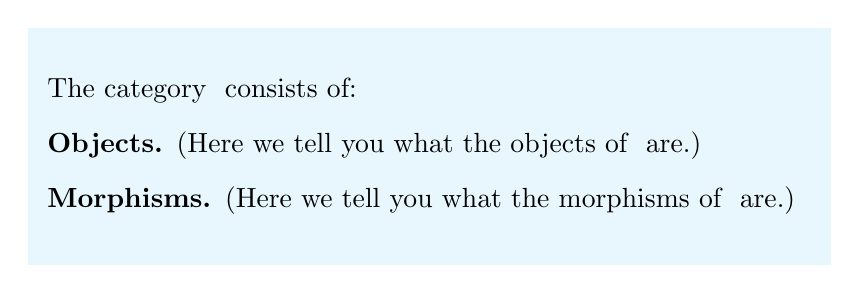
\begin{tikzpicture}
            \filldraw[ProcessBlue!10] (-0.42\textwidth, -1.5) rectangle (0.42\textwidth, 1.5);
            \node at (0,0){
                \begin{minipage}{0.8\textwidth}
                    The category $\cc$ consists of:
                    \begin{description}
                        \item[Objects.] (Here we tell you what the objects of $\cc$ are.)
                        \item[Morphisms.] (Here we tell you what the morphisms of $\cc$ are.)
                    \end{description}
                \end{minipage}
            };
        \end{tikzpicture}
    \end{center}
    This is simply to avoid a lot of unnecessary 
    words to describe a category (e.g. ''the objects of this category are... the morphisms of this category are...'').

    \begin{example}
        The canonical example of a category is the \textbf{category of sets}, denoted 
        as $\Set$, which we can describe as 
        \begin{description}
            \item[Objects.] All sets $X$.\footnote{There's a minor issue with saying this. We will address it, but not for now.} 
            \item[Morphisms.] All functions between sets $f: X \to Y$. 
        \end{description}
        Because most of mathematics is based in set theory, we shall see that while this is a fairly 
        simple category, it is one of the most useful. 
    \end{example}

    \textbf{A tip moving forward:} When dealing with any abstract construction, it is a common 
    strategy to keep a ``canonical example'' of such an abstract construction in your head. 
    For many people, they often use $\Set$ as the image in their head when they imagine a category. 
    This is fine, but one should be cautioned: 
    in general, categorical objects are not sets. 
    Furthemore, morphisms are in general not functions.
    This might be strange, but you will get used to it and it will eventually become natural to you.
    The moral of the story is:
    \begin{center}
        \begin{minipage}{0.7\textwidth}
            \textcolor{NavyBlue}{The canonical example of a category is $\Set$, but 
            \emph{in general} the objects of an arbitrary category $\cc$ are not sets, 
            and the morphisms are not functions. }
        \end{minipage}
    \end{center}

    \begin{example}
        The second canonical example is the \textbf{category of groups}, denoted 
        as $\grp$. This can be described as 
        \begin{description}
            \item[Objects.] All groups $(G, \cdot)$. Here, $\cdot: G \times G \to G$ is the group operation. 
            \item[Morphisms.] All group homomorphisms $\phi: (G, \cdot) \to (H, \cdot)$. 
            Specifically, set functions $\phi: G \to H$ where $\phi(g \cdot g') = \phi(g)\cdot \phi(g')$. 
        \end{description}        
        We again check this satisfies the axioms of a category. 
        \begin{description}
            \item[(1)] Each group $(G, \cdot)$ has a identity group homomorphism $\id_G: (G, \cdot) \to (G, \cdot)$ where 
            $\id_G(g) = g$. 
            \item[(2)] The function composition of two group homomorphisms $\phi: (G, \cdot) \to (H, \cdot)$ and $\psi: (H, \cdot) \to (K, \cdot)$ 
            is again a group homomorphism where $(\psi \circ \phi)(g) = \psi(\phi(g))$. This is because 
            \begin{align*}
                (\psi \circ \phi)(g \cdot g')&=
                \psi(\phi(g \cdot g'))\\ 
                &= \psi(\phi(g)\cdot \phi(g')) \\
                &= \psi(\phi(g)) \cdot \psi(\phi(g'))\\
                &= (\psi \circ \phi)(g) \cdot (\psi \circ \phi)(g).
            \end{align*}
            \item[(3)] Function composition is associative; therefore, composition of group homomorphisms is associative.
            \item[(4)] If $\phi: (G, \cdot) \to (H, \cdot)$ is a group homomorphism, then 
            $\id_H \circ \phi = \phi \circ \id_G = \phi$.
        \end{description}
        Therefore we see that this is a category. We will later see that this category possesses 
        many convenient and interesting properties. 
    \end{example}

    \begin{example}
        The third canonical example is the \textbf{category of topological spaces}, 
        denoted $\top$. We describe this as 
        \begin{description}
            \item[Objects.] All topological spaces $(X, \tau)$ where $\tau$ is a topology on the set $X$. 
            \item[Morphisms.] All continuous functions $f: (X, \tau) \to (Y, \tau')$.   
        \end{description}
        The reader can show that this too satisfies the axioms of a category.
    \end{example}

    We now consider some abstract examples. While abstract, they are nevertheless important 
    examples in their own right. They also illustrate that categories can be finite, 
    which may counter the intuition the reader might have of categories being ``infinte.''

    \begin{example}
        In this example we introduce the three most basic categorical structures. 
        The first, and most important of the three, is the \textbf{single object} or \textbf{initial category}
        $\bm{1}$, which is the category where: 
        \begin{description}
            \item[Objects.] A single object, abstractly denoted as $\bullet$.
            \item[Morphisms.] A single identity morphism $\id_{\bullet}: \bullet \to \bullet$. 
        \end{description}
        The identity of $\bullet$ does not matter; it is an abstract object. This is similar to how 
        a one point set is denoted as $\{*\}$ and we don't really care what $*$ is. 
        \\

        The second category is the \textbf{arrow category}, denoted as $\bm{2}$, which we can 
        describe as 
        \begin{description}
            \item[Objects.] Two objects $\textcolor{NavyBlue}{\bullet}$
            and $\textcolor{Orange}{\bullet}$
            \item[Morphisms.] Two identity morphisms $\id_{\textcolor{NavyBlue}{\bullet}}: \textcolor{NavyBlue}{\bullet}  \to \textcolor{NavyBlue}{\bullet} $ 
            and $\id_{\textcolor{Orange}{\bullet} }: \textcolor{Orange}{\bullet}  \to \textcolor{Orange}{\bullet}$ and one 
            nontrivial morphism $f: \textcolor{NavyBlue}{\bullet} \to \textcolor{Orange}{\bullet}$. 
        \end{description}
        Here we color our abstract objects to clarify that these objects are distinct.
        \\ 
        Finally, we have the category \textbf{triangle category}, denoted as $\bm{3}$, which 
        can be describe as 
        \begin{description}
            \item[Objects.] Three distinct objects $\textcolor{NavyBlue}{\bullet}, \textcolor{Orange}{\bullet}, \textcolor{Purple}{\bullet}$ 
            \item[Morphisms.] Three identity morphisms, and three nontrivial morphisms: 
            $f: \textcolor{NavyBlue}{\bullet} \to \textcolor{Purple}{\bullet}$, 
            $g: \textcolor{Purple}{\bullet} \to \textcolor{Orange}{\bullet}$ and $h: \textcolor{NavyBlue}{\bullet} \to \textcolor{Orange}{\bullet}$.
        \end{description}
        In this category, we define $h = g \circ f$ so that this is closed under composition. Note that 
        if we did not include the existence of $h$, then this would not be closed under composition, 
        and hence it would not even be a category.

        We can picture all three categories as below. 
        \begin{center}
            \begin{tikzpicture}
                \begin{scope}
                    \filldraw[rounded corners, Yellow!30]
                    (-2, -1.5) rectangle (2, 1.5);
                    \node at (0,0){
                        \begin{tikzcd}
                            \bullet \arrow[out=120,in=60,looseness=3,loop, "\id_{\bullet}"]
                        \end{tikzcd}
                    };
                    \node at (-1.5, 1) {$\bm{1}$};
                \end{scope}
                \begin{scope}[xshift = 5cm]
                    \filldraw[rounded corners, Yellow!30]
                    (-2, -1.5) rectangle (2, 1.5);
                    \node at (0,0){
                        \begin{tikzcd}
                            \textcolor{NavyBlue}{\bullet} 
                            \arrow[out=120,in=60,looseness=3,loop, "\id_{\textcolor{NavyBlue}{\bullet}}"]
                            \arrow[r, "f"]
                            &
                            \textcolor{Orange}{\bullet}
                            \arrow[out=120,in=60,looseness=3,loop, "\id_{\textcolor{Orange}{\bullet}}"]
                        \end{tikzcd}
                    };
                    \node at (-1.5, 1) {$\bm{2}$};
                \end{scope}
                \begin{scope}[xshift=11cm]
                    \filldraw[rounded corners, Yellow!30]
                    (-3, -1.5) rectangle (3, 1.5);
                    \node at (0,0){
                        \begin{tikzcd}
                            &
                            \textcolor{Purple}{\bullet}
                            \arrow[out=120,in=60,looseness=3,loop, "\id_{\textcolor{Purple}{\bullet}}"]
                            \arrow[dr, "g"]
                            &
                            \\
                            \textcolor{NavyBlue}{\bullet}
                            \arrow[out=120,in=60,looseness=3,loop, "\id_{\textcolor{NavyBlue}{\bullet}}"]
                            \arrow[ur, "f"]
                            \arrow[rr, swap, "g \circ f"]
                            &
                            &
                            \arrow[out=120,in=60,looseness=3,loop , "\id_{\textcolor{Orange}{\bullet}}"]
                            \textcolor{Orange}{\bullet}
                        \end{tikzcd}
                    };
                    \node at (-2.5, 1) {$\bm{3}$};
                \end{scope}
            \end{tikzpicture}
        \end{center}
    \end{example}

    Our first step in category theory has been introducing the axioms and showing 
    some simple examples. We now take our second step by moving on to more basic 
    concepts of category theory by making a few comments about categories. 

    \begin{definition}
        Let $\cc$ be a category. We say that $\cc$ is 
        \begin{itemize}
            \item \textbf{Finite} if there are only finitely many objects 
            and finitely many morphisms. 
            \item \textbf{Locally Finite} if, for every pair of objects 
            $A, B$, the set $\hom_{\cc}(A, B)$ is finite. 
            \item \textbf{Small} if the collection of objects and collections of morphisms 
            assemble into a set. 
            \item \textbf{Locally Small} if $\hom_{\cc}(A, B)$ is a set for every 
            pair of objects $A, B$. 
            \item \textbf{Large} if $\cc$ is not locally small. That is, the objects and 
            morphisms do not form a set. 
        \end{itemize}
    \end{definition}

    Such terminology proves to be useful, since we have seen that categories come in different sizes. 
    For example, the categories $\bm{1}, \bm{2},$ and $\bm{3}$ are finite categories.
    However, recall Russel's Paradox, so that the collection of all sets is not a set. 
    Therefore, $\Set$ is a large category.
    
    We now introduce the concept of a \emph{subcategory}, which is also extremely useful to include in our vocabularly. 
    \begin{definition}
        Let $\cc$ be a category. We say a category $\mathcal{S}$ is a \textbf{subcategory of $\cc$}
        if
        \begin{description}
            \item[(1)] $\ss$ is a category, with composition the same as $\cc$
            \item[(2)] The objects and morphisms of $\ss$ are contained in the collection of objects 
            and morphisms of $\cc$. 
        \end{description}
        Furthermore, we say $\ss$ is a \textbf{full subcategory} if we additionally have that 
        \begin{description}
            \item[(3)] For each pair of objects $A, B \in \ss$, we have that $\hom_{\ss}(A, B) = \hom_{\cc}(A, B)$.  
        \end{description}
        More informally, $\ss$ is full if it ``contains all of its morphisms.''
    \end{definition}

    \begin{example}
        Let $\ab$ be the category described as 
        \begin{description}
            \item[Objects.] All abelian groups $(G, \cdot)$
            \item[Morphisms.] Group homomorphisms.  
        \end{description}
        Then $\ab$ is a subcategory of $\grp$. Futhermore, $\ab$ 
        is a full subcategory of $\grp$. This observation also applies to 
        \begin{itemize}
            \item \textbf{FinGrp}, the category of finite groups 
            \item \textbf{FindAb}, the category finite abelian groups
            \item $\ab_{\text{TF}}$, the category of torsion-free abelian groups 
        \end{itemize}

        However, none of these categories are subcategories of $\Set$. In fact, 
        many categories which are based in set theory are not actually subcategories 
        of $\Set$. This is because the objects of categories such as $\grp$ or $\top$
        are not just sets, but are sets with extra data (such as a binary operation or a topology).  

    \end{example}

    \begin{example}
        Let $\ring$ be the category described as 
        \begin{description}
            \item[Objects.] Unital rings $(R, +, \cdot)$. That is, rings $R$ with a multiplicative identity 1 that is not 
            equal to its additive identity 0. 
            \item[Morphisms.] (Unit preserving) Ring homomorphisms $\phi: R \to R'$. 
            That is, functions $\phi: R \to R'$ such that 
            \begin{itemize}
                \item $\phi(a + b) = \phi(a) + \phi(b)$
                \item $\phi(a \cdot b) \phi(a) \cdot \phi(b)$ 
                \item $\phi(0_R) = 0_{R'}$ and $\phi(1_R) = 1_{R'}$.
            \end{itemize} 
        \end{description}
        For a ring $R$ we know that $(R, +)$ is an abelian group, and we know that 
        every ring homomorphism is technically a group homomorphism between abelian groups.
        However, it is not 
        the case that $\ab$ is a subcategory of $\ring$. This is because while 
        every ring is technically an abelian group, abelian groups on their own are not rings. 
    \end{example}

    We now introduce a convenient categorical construction which will serve to be useful to us 
    from here on out. 

    \begin{definition}
        Let $\cc, \dd$ be categories. Then we can form the \textbf{product category} where 
        we have that 
        \begin{description}
            \item[Objects.] Pairs $(C, D)$ with $C \in \cc$ and $D \in \dd$.
            \item[Morphisms.] Pairs $(f, g)$ where $f: C \to C'$ and $g: D \to D'$ are morphisms in $\cc$ and $\dd$.    
        \end{description}
        To define composition in this category, suppose we have composable morphisms in $\cc$ 
        and $\dd$ as below. 
        \begin{center}
            \begin{tikzpicture}
                \filldraw[rounded corners, yellow!30]
                (-3.75,0.25) rectangle (3.75,2.5);
                \node at (-2.75, 2){$\cc$};
                \node at (0,1.25){
                    \begin{tikzcd}[column sep = 1.4cm, row sep =  1.4cm]
                        \cdots
                        &[-1.5cm] 
                        C_1
                        \arrow[r, "f"]
                        \arrow[rr, bend left, "f' \circ f"]
                        &
                        C_2
                        \arrow[r, "f'"]
                        &
                        C_3
                        &[-1.5cm]
                        \cdots
                    \end{tikzcd}
                };
                \begin{scope}[xshift = 8cm]
                    \filldraw[rounded corners, yellow!30]
                    (-3.75,0.25) rectangle (3.75,2.5);
                    \node at (-3, 2){$\dd$};
                    \node at (0,1.25){
                        \begin{tikzcd}[column sep = 1.4cm, row sep =  1.4cm]
                            \cdots
                            &[-1.5cm]
                            D_1
                            \arrow[r, "g"]
                            \arrow[rr, bend left, "g' \circ g"]
                            &
                            D_2
                            \arrow[r, "g'"]
                            &
                            D_3   
                            &[-1.5cm]
                            \cdots           
                        \end{tikzcd}  
                    };
                \end{scope}
            \end{tikzpicture}                
        \end{center}
        Then the morphisms $(f, g)$ and $(f', g')$ in $\cc \times \dd$ 
        are composable too, and their composition is defined as $(f', g') \circ (f , g) = ( f' \circ f, g' \circ g)$.
        \begin{center}
            \begin{tikzpicture}
                \filldraw[rounded corners, yellow!30]
                (-5,-2.25) rectangle (5,0.25);
                \node at (-3.5, -0.25){$\cc \times \dd$};
                \node at (0,-1){
                    \begin{tikzcd}[column sep = 1.4cm, row sep =  1.4cm]
                        \cdots
                        &[-1.5cm]
                        (C_1,D_1) 
                        \arrow[r, "{(f,g)}"]
                        \arrow[rr, bend left, "{(f', g') \circ (f, g) = (f' \circ f, g' \circ g)}"]
                        &
                        (C_2, D_2)
                        \arrow[r, "{(f',g')}"]
                        &
                        (C_3, D_3)
                        &[-1.5cm]
                        \cdots
                    \end{tikzcd}  
                };
            \end{tikzpicture}
        \end{center}     
    \end{definition}

    Note that we can form even larger products of categories; we don't have to stop at two! 
    But this will be explored later. For now, we can just be happy with this 
    new tool because it allows us to be build new categories from the old ones that we already 
    know. 

    \begin{example}
        A useful example of a product involves the category $\Set\times\Set$ which 
        we can describe as 
        \begin{description}
            \item[Objects.] Pairs of sets $(X, Y)$.
            \item[Morphisms.] Pairs of functions $(f, g)$. 
        \end{description}
        Such product constructions are useful because in general, algebraic operations of any kind 
        require a product. For example, to talk about a group $(G, \cdot)$, 
        one needs a binary operator, i.e. a function $\cdot: G \times G \to G$.
        Hence to talk to generalize operations on categories, we need to talk about products. 
        For example, with $\Set\times\Set$, we can talk about the product of two sets 
        as a mapping $\times: \Set \times \Set \to \Set$ where $(A, B) \mapsto A \times B$. 
    \end{example}










    \newpage
    \section{Examples of Categories}

    Now that we have some idea of basic categories and a few examples in mind on 
    how they work, we introduce more examples in this section to deepen our understanding.
    Categories are extremely abundant in mathematics, so it is not difficult to 
    find examples.

    Without proof, we comment that the categories below truly form categories. 
    To discuss these categories, we will use the notation in the leftmost column.
    \begin{center}
        \begin{tabular}{ |p{1.5cm}||p{6cm}||p{8cm}|  }
            \hline
            Category & Objects & Morphisms\\
            \hline
            $\finset$ & Finite sets $X$ & Functions $f: X \to Y$\\
            $\vect_K$ & Vector spaces over $k$ & Linear transformations $T: V \to W$\\
            $\mon$ & Monoids $(M, \cdot)$ & Monoid homomorphisms $\psi: M \to M'$\\
            \textbf{FinGrp} & Finite Groups & Group homomorphisms $\phi: (G, \cdot) \to (H, \cdot)$\\
            $\ab$ & Abelian Groups $(G, \cdot)$ & Group homomorphisms\\
            \textbf{FinAb} & Finite Abelian Groups $(G, \cdot)$ & Group homomorphisms\\
            \textbf{Ring} & Rings $(R, \cdot, +)$ & Ring homomorphisms $\phi: (R, \cdot, +) \to (S, \cdot, +)$\\
            \textbf{CRing} & Commutative Rings $(R, \cdot, +)$ & Ring homomorphisms \\
            $\ring$ & Rings $(R, \cdot, +)$ with identity $1 \ne 0$ & Ring homomorphisms\\
            $R\mod$& $R$-modules $(M, +)$ & $R$-module homomorphisms\\
            $\fld$ & Fields $k$ & Field homomorphisms\\
            $\top^*$ & Topological spaces $(X, x_0)$ with basepoint $x_0 \in X$  & Continuous functions preserving basepoints\\
            \textbf{Toph} & Topological spaces $(X, \tau)$ & Homotopy equivalence classes \\
            \textbf{Haus} & Hausdorff topological spaces $(X, \tau)$ & Continuous functions\\
            \textbf{CHaus} & Compact Hausdorff topological spaces $(X, \tau)$ & Continuous functions\\
            \textbf{DMan} & Differentiable manifolds $M$ & Differentiable functions $\phi: M \to M'$\\
            \textbf{LieAlg} & Lie algebras $\mathfrak{g}$ & Lie algebra homomorphisms\\
            \textbf{Grph} & Graphs $(G, E, V)$ & Graph homomorphisms\\
            \hline
           \end{tabular}
    \end{center}

    Now that we are aquainted with some of the categories that we'll be working with, 
    we'll introduce more interesting categories that become useful. However, 
    these categories are less trivial than the ones above, i.e it takes a bit of work 
    to see how they form into categories. 


    \begin{example}
        Let $X$ be a nonempty set. We can regard $X$ as a 
        category where 
        \begin{description}
            \item[Objects.] All elements of $X$.
            \item[Morphisms.] All morphisms are identity morphisms, and there are 
            no morphisms between any two distinct objects.  
        \end{description}
        This category, while fairly trivial, is called a \textbf{discrete category}.
    \end{example}

    \begin{example}
        Consider any of the categories $\mon$, $\grp$, $\ring$, or 
        $R\mod$. For any object of these categories, we can create 
        the notion of a \emph{grading}. Such a concept is a useful algebraic construction which 
        appears in different areas of mathematics. For simplicity, we'll consider a grading 
        on a group.

        A group $G$ is said to be \textbf{$\mathbb{N}$-graded} if there exists a family 
        of groups $G_1, G_2, \dots, G_n, \dots$ such that $G = \bigoplus_{i=1}G_i$.
        An example of this is the group $(\mathbb{R}[x], +)$, the single variable polynomials 
        in one variable. To see that this is graded, observe that any 
        polynomial $p(x)$ is of the form
        \[
            p(x) = a_0 + a_1x + a_2x^2 + \cdots + a_{n}x^n.
        \]
        Note that $p(x)$ consists of ``components'', i.e., different powers 
        of $x$. If we let 
        \[
            \mathbb{R}_n[x] = \{ax^n \mid a \in \mathbb{R}\}    
        \]
        then we see that $\mathbb{R}[x] = \bigoplus_{i = 0}\mathbb{R}_n[x]$. 

        More generally, if $\lambda$ is an indexing set, we say a group $G$ is \textbf{$\lambda$-graded} 
        if there is a family of groups $G_i, i \in \lambda$ such that $G = \bigoplus_{i \in \lambda}G_i$.
        In addition, if $G = \bigoplus_{i \in \lambda}G_i$ and $H = \bigoplus_{i \in \lambda}H_i$ 
        are two graded groups such that $\phi_i:G_i \to H_i$ is a group homomorphism, 
        then we say $\phi: G \to H$ is a \textbf{$\lambda$-graded homomorphism}.

        With that said, we can define the category of graded groups to be the category 
        \textbf{GrGrp}, (read as ``graded groups'') described as 
        \begin{description}
            \item[Objects.] $\lambda$-graded groups $G = \bigoplus_{i \in \lambda}$ 
            for some set $\lambda$ 
            \item[Morphisms.] Graded homomorphisms between graded groups.  
        \end{description}
        As we said before, this produces many graded categories, including \textbf{GrMon}, 
        \textbf{GrRing}, $\textbf{GrMod}_R$ etc.
    \end{example}

    \begin{example}
        A monoid is a set $M$ equipped with an operation $\cdot: M \times M \to M$ and 
        an identity $e$ such that $e\cdot m = m \cdot e = m$ for all $m \in M$. In other words, 
        monoids are like groups, in that we drop the requirement of an inverse. 

        Let $\cc$ be a category with one object; denote this object as $\bullet$. 
        As we have one object, we have one homset. We can then interpret $M$ as a category
        by setting 
        \[
            \hom_{\cc}(\bullet, \bullet) = M.   
        \]
        Thus each $m \in M$ corresponds to a morphism.
        So,
        we can write each morphism in the category as $f_{m}: \bullet \to \bullet$ 
        for some $m \in M$. 
        We then write $f_{e} = 1_{\bullet}$, the identity, and more generally 
        define composition in the category as
        \[
            f_m \circ f_{m'} = f_{m \cdot m'}.   
        \]
        Since $M$ is a monoid, and its multiplication is associative, we see that composition defined in this way is also associative. 
        Further, for each $f_m$, we have that 
        \[
            f_{e} \circ f_m =  f_m \circ f_{e} = f_m
        \]
        since $e \cdot m = m \cdot e = m$ in the monoid $M$. Thus we can interpret monoids 
        as one object categories. 
    \end{example}

    \begin{definition}
        A category $\mathcal{P}$ is said to be \textbf{thin} or a \textbf{preorder}
        if there is \textbf{at most} one morphism $f:  A \to B$ for each $A, B \in \mathcal{P}$. 
    \end{definition}\label{definition:thin-category}
    The simplest thin categories are of the form below 
    \begin{center}
        \begin{tikzpicture}
            \filldraw[rounded corners, Yellow!30]
            (-4, -1.25) rectangle (3, 1.25);
            \node at (0,0){
                \begin{tikzcd}
                    A 
                    \arrow[r]
                    &
                    B
                    \arrow[r]
                    &
                    C
                    \arrow[r]
                    &
                    \cdots 
                    &
                \end{tikzcd}
            };
            \node at (-3.5, 0.8){$\pp$};
        \end{tikzpicture}
    \end{center}
    but they may also have more complex shapes such as the category below. 
    \begin{center}
        \begin{tikzpicture}
            \filldraw[rounded corners, Yellow!30]
            (-3.5, -2.5) rectangle (3.5, 2.5);
            \node at (0,0){
                \begin{tikzcd}
                    B
                    &
                    C
                    &
                    D
                    \\
                    &
                    A
                    \arrow[u]
                    \arrow[d]
                    % \arrow[l]
                    % \arrow[r]
                    \arrow[ur]
                    \arrow[ul]
                    \arrow[dr]
                    \arrow[dl]
                    &
                    \\
                    E
                    &
                    F
                    &
                    G
                \end{tikzcd}
                };
            \node at (2, 1.8) {\rotatebox[origin=c]{70}{$\ddots$}};
            \node at (-2.1, 1.8) {$\ddots$};
            \node at (-2.2, -1.8) {\rotatebox[origin=c]{70}{$\ddots$}};
            \node at (2.2, -1.6) {$\ddots$};
            \node at (0, 2.1) {$\vdots$};
            \node at (0, -1.9) {$\vdots$};
            % \node at (2.3, 0.2) {$\cdots$};
            % \node at (-2.3, 0.2) {$\cdots$};
            \node at (-3, 1.9){$\pp$};
    \end{tikzpicture}
    \end{center}
    Thin categories are very common since we often times only care about one single 
    type of relation between any two objects. An example of such a relation is a binary relation; 
    for any two real numbers $x, y \in \rr$, we know that either $x \le y$ or $y \le x$. 

    This intuition is actually not very far off. Given a thin category $\mathcal{P}$,
    define the binary relation $\le$ on the objects $\ob(\mathcal{P})$ as follows. 
    For any pair of objects $A, B \in \mathcal{P}$, we have that 
    \[
        A \le B \text{ if and only if there exists an morphism } A \to B. 
    \]
    Some things are to be said about this relation:
    \begin{itemize}
        \item For each object $A$, 
        there always
        exists a morphism $A \to A$ (namely, the identity). This implies
        that $A \le A$ for all objects $A$, so that $\le$ is reflexive.

        \item If $f: A \to B$ and $g: B \to C$, then we have that 
        $A \le B$ and $B \le C$. Since we may compose morphisms, we 
        have that $g \circ f: A \to C$. Therefore, $A \le C$, so that $\le$ 
        $\le$ is transitive.
    \end{itemize}
    Hence, $\mathcal{P}$ is really just a set with a reflexive and transitive
    binary relation. However, this is exactly the definition of a \textbf{preorder}!
    Therefore, preorders $P$ can be regarded as categories with at most 
    one morphism between any two objects, and vice versa.

    Preorders can also turn into \textbf{partial orders}, which
    have the axiom that 
    \[
        \text{if } p \le p' \text{ and } p' \le p \text{ then } p = p'.
    \]
    or \textbf{linear orders}, where for any $p,  p'$ we have that $p \le
    p'$ \textbf{or} $p' \le p$.

    \begin{example}
        Here we introduce some examples of thin categories.
        \begin{description}
            \item[Natural Numbers.] 
            The sets $\{1, 2, \dots, n\}$ for any $n \in N$ are
            linear orders, each of which forms a category as pictured below.
            \begin{center}
                \begin{tikzcd}
                    1 \arrow[r] \arrow[out=120,in=60,looseness=3,loop]
                    &
                    2 \arrow[r] \arrow[out=120,in=60,looseness=3,loop]
                    &
                    3 \arrow[r] \arrow[out=120,in=60,looseness=3,loop]
                    &
                    \dots \arrow[r] 
                    & 
                    n \arrow[scale = 2.5, out=123,in=57,looseness = 3, loop]
                \end{tikzcd}
            \end{center}
            In this figure, the loops represent the trivial identity functions.

            This example can also be generalized to include $\mathbb{N}, \mathbb{Z}, 
            \mathbb{Q},$ and $\mathbb{R}$. 

            \item[Subsets.] 
            Let $X$ be a set. Then one can form a category $\text{Subsets}(X)$ where the 
            objects are subsets of $X$ and the morphisms are inclusion morphisms. Hence,
            there is at most one morphism between any two sets.

            Since there is at most one morphism between any two objects of the 
            category, we see that this forms a thin category, and hence a partial ordering. 
            What this then tells us is that subset containment determines an ordering, 
            specifically a partial ordering. 

            \item[Open Sets.]   
            Let $(X, \tau)$ be a topological space. Define the category 
            $\open(X)$ to be the category whose objects are the open sets of $X$ 
            and morphisms $U \to V$ are inclusion morphisms $i: U \to V$ whenever $U \subset V$.
            Hence, there is at most one morphism between any two open sets, so that this 
            also forms a preorder.
            
            \item[Subgroups.] 
            Let $G$ be a group. We can similarly define the category 
            $\textbf{SbGrp}(G)$ to be the category whose objects consists 
            of subgroups $H \le G$, and whose morphisms are inclusion homomorphisms.
            This is just like the last example; and, as in the last example, 
            there is at most one morphism between any two subgroups $H, K$ of $G$ 
            (either $i: H \to K$ or $i: K \to H$). Hence, we can place a partial ordering 
            on this, so that subgroup containment is a partial ordering.

            \item[Ideals.]
            Let $R$ be a ring. Then we can form a category $\textbf{Ideals}(R)$ 
            whose objects are the ideals $I$ of $R$ and whose morphisms are inclusion 
            morphisms. As we've seen, this forms a thin category. 
        \end{description}

    \end{example}

    \begin{example}
        Let $B_n$ be the set of braids on $n$ strands. Recall that 
        $B_n$ forms a group where the group product is composition, and where the identity is simply 
        $n$ parallel strands. Each braid group actually has a nice presentation:
        \[
            B_n = \left< \sigma_1, \dots, \sigma_{n-1} \mid \sigma_i\sigma_{i+1}\sigma_{i} = \sigma_{i+1}\sigma_{i}\sigma_{i+1}^{(\texttt{1})}, \sigma_i\sigma_j = \sigma_j\sigma_i^{(\texttt{2})} \right>   
        \]
        where (\texttt{1}) holds only when $1 \le i \le n - 2$ and (\texttt{2}) hold only when 
        $|i - j| > 1$. These two laws are imposed so that they match our geometric intuition, so that
        if we were to replace the strands with \emph{real}, phyiscal 
        ropes then they would behave the same way.

        Each generator $\sigma_i$ is interpreted as swapping the $i$-th strand \emph{over}
        the $(i+1)$-th strand, while $\sigma_i$ is swapping the $(i+1)$-th strand over the $i$-th strand.
        Below are some example generators.
        \begin{center}
            \begin{tikzpicture}
                \pic[local bounding box=my braid,braid/.cd, 
                number of strands = 2, % number of  strands
                thick,
                name prefix=braid]
                {braid={ s_1}}; %the generators
                \draw[thick] % draws the top/bottom bars
                ([xshift=-1ex]my braid.north west) --  ([xshift=1ex]my braid.north east)
                ([xshift=-1ex]my braid.south west) --  ([xshift=1ex]my braid.south east);
                % labels the top bar
                \foreach \n in {1,...,2}{
                    \node at (braid-\n-s)[yshift = 0.3cm] {\n};
                } 
                % labels the bottom bar
                \foreach \n in {1,...,2}{
                    \node at (braid-\n-e)[yshift = -0.3cm] {\n};
                } 
            \end{tikzpicture}
            \hspace{1cm}
            \begin{tikzpicture}
                \pic[local bounding box=my braid,braid/.cd, 
                number of strands = 2, % number of  strands
                thick,
                name prefix=braid]
                {braid={ s_1^{-1}}}; %the generators
                \draw[thick] % draws the top/bottom bars
                ([xshift=-1ex]my braid.north west) --  ([xshift=1ex]my braid.north east)
                ([xshift=-1ex]my braid.south west) --  ([xshift=1ex]my braid.south east);
                % labels the top bar
                \foreach \n in {1,...,2}{
                    \node at (braid-\n-s)[yshift = 0.3cm] {\n};
                } 
                % labels the bottom bar
                \foreach \n in {1,...,2}{
                    \node at (braid-\n-e)[yshift = -0.3cm] {\n};
                } 
            \end{tikzpicture}
            \hspace{1cm}
            \begin{tikzpicture}
                \pic[local bounding box=my braid,braid/.cd, 
                number of strands =3, % number of  strands
                thick,
                name prefix=braid]
                {braid={ s_2 }}; %the generators
                \draw[thick] % draws the top/bottom bars
                ([xshift=-1ex]my braid.north west) --  ([xshift=1ex]my braid.north east)
                ([xshift=-1ex]my braid.south west) --  ([xshift=1ex]my braid.south east);
                % labels the top bar
                \foreach \n in {1,...,3}{
                    \node at (braid-\n-s)[yshift = 0.3cm] {\n};
                } 
                % labels the bottom bar
                \foreach \n in {1,...,3}{
                    \node at (braid-\n-e)[yshift = -0.3cm] {\n};
                } 
            \end{tikzpicture}
            \hspace{1cm}
            \begin{tikzpicture}
                \pic[local bounding box=my braid,braid/.cd, 
                number of strands =4, % number of  strands
                thick,
                name prefix=braid]
                {braid={ s_3^{-1} }}; %the generators
                \draw[thick] % draws the top/bottom bars
                ([xshift=-1ex]my braid.north west) --  ([xshift=1ex]my braid.north east)
                ([xshift=-1ex]my braid.south west) --  ([xshift=1ex]my braid.south east);
                % labels the top bar
                \foreach \n in {1,...,4}{
                    \node at (braid-\n-s)[yshift = 0.3cm] {\n};
                } 
                % labels the bottom bar
                \foreach \n in {1,...,4}{
                    \node at (braid-\n-e)[yshift = -0.3cm] {\n};
                } 
            \end{tikzpicture}
            
            \emph{$\sigma_1$ on two strands; $\sigma^{-1}$ on two stands; $\sigma_2$ on three strands; $\sigma_3$ on four strands.}
        \end{center}
        The reason why we care about these generators is because every braid can be expressed 
        by over and under crossings (although such an expression may not be unique).
        Now, the group multiplication in this group is simply stacking of braids. For example, the braid
        \begin{center}
            \def\nstrands{4}
            \def\xcoord{0}
            \begin{tikzpicture}
                \pic[local bounding box=my braid,braid/.cd, 
                number of strands = 3, % number of  strands
                thick,
                name prefix=braid]
                {braid={ s_1 s_2 s_1}}; %the generators
                \draw[thick] % draws the top/bottom bars
                ([xshift=-1ex]my braid.north west) --  ([xshift=1ex]my braid.north east)
                ([xshift=-1ex]my braid.south west) --  ([xshift=1ex]my braid.south east);
                % labels the top bar
                \foreach \n in {1,...,3}{
                    \node at (braid-\n-s)[yshift = 0.3cm] {\n};
                } 
                % labels the bottom bar
                \foreach \n in {1,...,3}{
                    \node at (braid-\n-e)[yshift = -0.3cm] {\n};
                } 
            \end{tikzpicture}
        \end{center}
        can be obtained by stacking $\sigma_1, \sigma_2$ and then $\sigma_1$ again. 
        Hence, the  braid $\sigma_1\sigma_2\sigma_1$. 

        Now with the family of braid groups $B_1, B_2, \dots,$ we can form a category $\mathbb{B}$
        as follows. 
        \begin{description}
            \item[Objects.] Positive integers $1,2, \dots,$
            \item[Morphisms.] For any pair of positive integers $n,m$, we have that 
            \[
                \hom_{\mathbb{B}}(n,m) = 
                \begin{cases}
                    B_n & \text{if } n = m\\
                    \varnothing & n \ne m
                \end{cases}
            \]
        \end{description}
        Hence we only have morphisms $f: n \to m$ when $n = m$. Furthermore, each 
        morphism is a braid. Composition is then group multiplication. The identity for each 
        object $n$ is the identity braid of $n$ parallel strands. As group multiplication 
        is associative, the composition in this category is associative, so we see that this truly 
        does form a category. 
    \end{example}

    The following examples demonstrates again that morphisms are not always 
    functions, or mappings of some kind.

    \begin{example}
        Let $R$ be a ring with identity $1 \ne 0$. For every pair of positive 
        integers $m, n$, let $M_{m, n}(R)$ be the set of all $m \times n$ matrices. 
        Now recall that for an $m \times n$ matrix $A$ and a $n \times p$ matrix  $B$, 
        the product $AB$ is an $m \times p$ matrix.  
        \[
            \begin{pmatrix}
                a_{11} & a_{12} & \cdots & a_{1n}\\
                a_{21} & a_{22} & \cdots & a_{2n}\\
                \vdots & \vdots & \ddots & \vdots\\
                a_{m1} & a_{m2} & \cdots & a_{mn}
            \end{pmatrix}
            \begin{pmatrix}
                b_{11} & b_{12} & \cdots & b_{1p}\\
                b_{21} & b_{22} & \cdots & b_{2p}\\
                \vdots & \vdots & \ddots & \vdots\\
                b_{n1} & b_{n2} & \cdots & b_{np}
            \end{pmatrix}  
            =
            \begin{pmatrix}
                c_{11} & c_{12} & \cdots & c_{1p}\\
                c_{21} & c_{22} & \cdots & c_{2p}\\
                \vdots & \vdots & \ddots & \vdots\\
                c_{n1} & c_{n2} & \cdots & c_{np}
            \end{pmatrix}  
        \]
        where $\displaystyle c_{ij} = \sum_{k= 1}^{n}a_{ik}b_{kj}$. This can rephrased as saying that 
        we have a multiplication map as below.
        \[
            M_{m,n}(R)\times M_{n,p}(R) \to M_{m, p}(R)
        \]
        Since matrix multiplication is associative, we can also say that the above mapping 
        is associative. 

        This however should feel sort of similar to the process of composition, say for example in $\Set$, 
        where if we  have functions $f: X \to Y$  and $g: Y \to Z$ we obtain a function $g \circ f:
        X \to Z$. If we follow this intuition, we can consider a \emph{matrix} $A$ 
        of shape $m \times n$ as a morphism from $m \to n$. Similarly,
        $B$ can be regarded a morphism from $n \to p$. This together implies that 
        $AB$ is a morphism from $m \to p$. 
        This should feel strange, because we are used to thinking of a morphism as some kind 
        of function. But it works; we can form a category where  
        \begin{description}
            \item[Objects.] The objects are positive integers $m$.
            \item[Morphisms.] The morphisms are matrices. Specifically, for any pair of 
            objects $m,n$, 
            \[
                \hom_{\cc}(m, n) = M_{m, n}(R).
            \]
            Here, composition is simply matrix multiplication.
        \end{description}
        Observe now that our initial observation regarding matrix multiplication
        translates to a statement regarding whenever two matrices $A$ and $B$ are 
        "composable" (i.e., whenever we can multiply them). That is, 
        our mapping $M_{m,n}(R)\times M_{n,p}(R) \to M_{m, p}$ can be rephrased as composition
        \[
            \circ: \hom_{\cc}(m, n) \times \hom_{\cc}(n, p) \to \hom_{\cc}(m, p)
        \] 
        Associativity of matrix multiplication translates to associativity of composition. 
        Finally, note that for each object (positive integer) $n$, the identity morphism is 
        simply the identity matrix. 
        \[
            1_n  := I_n = 
            \begin{pmatrix}
                1 & 0 & 0  & \cdots & 0\\
                0 & 1 & 0  & \cdots & 0\\
                \vdots & \vdots & \vdots & \ddots & \vdots\\
                0 & 0 & 0 & \cdots & 1\\
            \end{pmatrix}.
        \]
        Thus we see that we have all the necessary ingredients to declare this to be a category. 
    \end{example}


    \begin{example}
        Let $G$ be a group, and recall that $G$ is equipped with some binary 
        operator $\cdot: G \times G \to G$ which satisfies associativity. 
        Because this is a two-variable function on $G$ every 
        $g \in G$ induces a map
        \[
            (-) \cdot g := f_g: G \to G \qquad 
        \]
        This then gives rise to a collection of maps $f_g: G \to G$ for each 
        $g \in G$, which we can picture as below. 
        \begin{center}
            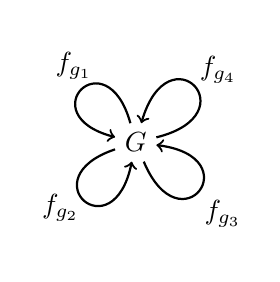
\begin{tikzpicture}
                \node at (0,0) (loop) {$G$};
                \begin{scope}[rotate= 55]
                    \draw[thick, <-] (loop) to [looseness=11, out=120,in=60,] node[above, xshift=-0.1cm] {$f_{g_1}$} (loop);
                \end{scope}
                \begin{scope}[rotate = 145]
                    \draw[thick, <-] (loop) to [looseness=15, out=120,in=60,] node[above, yshift=-0.4cm, xshift = -0.3cm] {$f_{g_2}$} (loop);
                    \begin{scope}[rotate = 80]
                        \draw[thick, <-] (loop) to [looseness=15, out=120,in=60,] node[above, yshift=-0.6cm, xshift = 0.3cm] {$f_{g_3}$} (loop);
                    \end{scope}
                \end{scope}
                \begin{scope}[rotate = 305]
                    \draw[thick, <-] (loop) to [looseness=12, out=120,in=60,] node[above, yshift=-0.1cm, xshift = 0.3cm] {$f_{g_4}$} (loop);
                \end{scope}
            \end{tikzpicture}
        \end{center}
        In particular, if $e\in G$ is the identity, then $f_e = 1_G$. 
        Moreover, composition of these maps is associative.
        Thus we can think of this as a category, specifically 
        one with one object, whose morphisms $f:G \to G$ are induced
        by the elements $g \in G$.
        Also, note that each such map is an isomorphism, since its inverse 
        is given by $(-) \cdot g^{-1}: G \to G$. 

        Now we can step up a level of generality. Let $X$ be a set, and 
        suppose we have a group action $\phi: X \times G \to X$. If we denote 
        $\phi(g, -):= \phi_h: X \to X$ for each $g \in G$, then since $\phi$ 
        is a group action we have that $\phi_g \circ \phi_{g'} = \phi_{g\cdot g'}$ 
        and $\phi_e = 1_X$. Hence composition is associative and we have a well-behaved
        identity morphism. Usually, when we draw group actions, we think of something 
        like this: 
        \begin{center}
            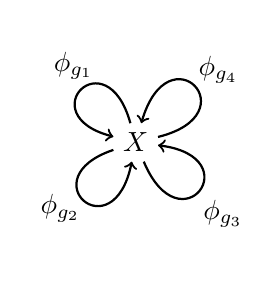
\begin{tikzpicture}
                \node at (0,0) (loop) {$X$};
                \begin{scope}[rotate= 55]
                    \draw[thick, <-] (loop) to [looseness=11, out=120,in=60,] node[above, xshift=-0.1cm] {$\phi_{g_1}$} (loop);
                \end{scope}
                \begin{scope}[rotate = 145]
                    \draw[thick, <-] (loop) to [looseness=15, out=120,in=60,] node[above, yshift=-0.4cm, xshift = -0.3cm] {$\phi_{g_2}$} (loop);
                    \begin{scope}[rotate = 80]
                        \draw[thick, <-] (loop) to [looseness=15, out=120,in=60,] node[above, yshift=-0.6cm, xshift = 0.3cm] {$\phi_{g_3}$} (loop);
                    \end{scope}
                \end{scope}
                \begin{scope}[rotate = 305]
                    \draw[thick, <-] (loop) to [looseness=12, out=120,in=60,] node[above, yshift=-0.1cm, xshift = 0.3cm] {$\phi_{g_4}$} (loop);
                \end{scope}
            \end{tikzpicture}
        \end{center}
        What we're seeing is that group actions can be phrased as a category with one object, 
        with morphisms as isomorphisms. This generalizes our previous discussion, which makes 
        sense since groups are trivial examples of group actions by setting $X = G$. 
    \end{example}


    {\large \textbf{Exercises}
    \vspace{0.2cm}}
    \begin{itemize}
        \item[\textbf{1.}] 
        Let $n$ be a positive integer, and consider a group $G$ such that 
        $g^n = 1$ for all elements $g \in G$. Show that if we take these groups to be 
        our objects, and group homomorphisms to be our morphisms, then 
        this forms a category $\grp_n$.
        \vspace{0.2cm}

        \item[\textbf{2.}] 
        Consider an infinite family of groups $G_1, G_2, \dots, G_n, \dots$
        Show that we have a category $\textbf{G}$ where
        \begin{description}
            \item[Objects.] The positive integers $1, 2, \dots, n, \dots$
            \item[Morphisms.] For any two positive integers $n,m$,  
            we define 
            \[
                \hom_{\textbf{G}}(n,m) = 
                \begin{cases}
                    G_n & \text{if } n = m\\
                    \varnothing & \text{otherwise}.
                \end{cases}  
            \] 
        \end{description}
        This example can be applied to many interesting families of groups, since they 
        often come graded (i.e., they often are indexed by the positive integers.)
        For instance, the braid groups $B_1, B_2, \dots,$ are such an example.
        \vspace{0.2cm}

        \item[\textbf{3.}] 
        Let $f: X \to Y$ be a function between two sets. 
        We say $f$ has the ``finite-to-one'' property if $f^{-1}(y)$ is always a 
        finite set for all $y \in Y$. Show that we have a (large) category,  denoted 
        $\Set_{FTO}$, where 
        \begin{description}
            \item[Objects.] All sets $X$.
            \item[Morphisms.] functions $f$ with the finite-to-one property. 
        \end{description}
        \vspace{0.2cm}

        \item[\textbf{4.}]
        Let $X$ and $Y$ be sets. A binary relation $R$ on $X$ and $Y$
        is any subset of $X \times Y$. For two elements 
        $x \in X, y \in Y$, we then write 
        $xRy$ if $(x,y) \in R$. Binary relations can be specialized to describe 
        functions and order relations in set theory.

        Show that we can form a category where 
        \begin{description}
            \item[Objects.] All sets $X$. 
            \item[Morphisms.] For any two sets $X,Y$, we write,
            by abuse of notation, $R: X \to Y$ as a morphism
            for each relation $R$ on $X$ and $Y$.
        \end{description}
        This category is called \textbf{Rel}, to indicate that it is the 
        category of relations.\\
        \emph{Hint:}  Define composition in this category as follows. Suppose 
        $R:X\to Y$ is a relation on $X$ and $Y$ and $P: Y \to Z$ is a binary relation on $Y$ and $Z$.
        Then the composite relation $Q: X \to Z$ is given by 
        \[
            Q = \{(x, z) \mid \text{there exist } y \in Y \text{ such that } (x,y)\in R, (y,z) \in P \}.
        \]

        \item[\textbf{5.}]
        Recall that for a two metric spaces $(M, d_M)$ and $(N, d_N)$, where 
        $d_M: M \times M \to M$ and $d_N: N \times N \to N$ are the metrics, 
        we say a function $f: M \to N$ is a \textbf{Lipschitz-1} map 
        with \textbf{Lipschitz constant} 1 if 
        \[
            d_N(f(x), f(y)) \le d_M(x, y)  
        \]
        for all $x, y \in M$. Using this concept, show that we have a category 
        where 
        \begin{description}
            \item[Objects.] Metric spaces $M$ 
            \item[Morphisms.] Lipschitz-1 maps with Lipschitz constant 1.   
        \end{description}
        This category is commonly denoted as \textbf{Met}.

        \item[\textbf{6.}]
        Let $G$ be a group. We say that $G$ acts on a set $X$ if we have a 
        function $\phi: G \times X \to X$ such that 
        \begin{itemize}
            \item[$\bullet$] $e \cdot x = x$
            \item[$\bullet$] $h\cdot (g \cdot x) = (hg)\cdot x$
        \end{itemize}
        Such an $X$ is sometimes called a \textbf{G-set}.
        Note here that we represent $\phi(g, x)$ as $g \cdot x$. Now suppose $X, Y$ are 
        two sets for which $G$ acts on. Then we define a morphism of $G$ sets to be a 
        function $f: X \to Y$ such that $f(g \cdot x) = g \cdot f(x)$. Such a map is called 
        $G$ equivariant. Show that we have 
        a category $G\textbf{-Sets}$ where 
        \begin{description}
            \item[Objects.] All $G$-sets (i.e., sets with a group action by $G$)
            \item[Morphisms.] $G$ equivariant maps. 
        \end{description}
    \end{itemize}

    \newpage
    \section{Paths and Diagrams in Categories}
    In this section we give an overview of the concept of a \emph{path} and 
    of a \emph{diagram} within a category, which are concepts that are exactly 
    what they sound like. 
    This is usually a discussion that is usually glossed over,
    which is a huge mistake since diagrams are used everywhere in mathematics. 
    They'll appear in nearly every section from this point on, and any good book 
    on category theory will have dozens of diagrams. In short, they 
    are extremely indespensible. 

    % At best, authors will offer vague definitions of a diagram 
    % (I will offer ``the'' vague definition in the next section for completeness)
    % which ultimately offer no insight into the concept of a diagram. 
    % The rationale for upholding the bad definition of a diagram is 
    % the ``Well, it's obvious!'' and ``Well, we know what it \emph{looks} like''
    % logic (This is ``lazy mathematics;'' the opposite is ``abstract nonsense.''). 
    % However, a general theme of mathematics is that just because you know what 
    % something \emph{looks like} doesn't mean you actually \emph{know and understand}
    % what that thing is, and slapping a lazy definition onto it is not 
    % a solution. This is a fundamental lesson in basic undergraduate mathematics. 
    % The moral is that if you cannot rigorously define what something is (or, at 
    % least, if one has not wrestled with the rigorous definition at least once), 
    % then there is no actual true understanding. 

    So, we set off to do a justice to the important concepts of paths and diagrams. 
    However, I've kept the pragmatic reader in mind and have avoided making 
    this discussion abstract and irrelevant. 

    First, we form some intuition on what exactly a diagram is. 
    Informally, a diagram in a category $\cc$ consists of a finite sequence 
    of arrows between objects. Below are some diagrams. 
    \begin{center}
        \begin{tikzcd}[row sep = 1.4cm, column sep = 1.4cm]
            A 
            \arrow[r, "\phi"]
            \arrow[d, swap, "\sigma"] 
            & 
            B
            \arrow[d, "\psi"]
            \\
            C \arrow[r, swap, "\tau"]
            & 
            D
        \end{tikzcd}
        \hspace{0.6cm}
        \begin{tikzcd}[row sep = 1.4cm, column sep = 1.4cm]
            & Y \arrow[dr, "g"]&\\
            X \arrow[rr, swap, "g \circ f"]
            \arrow[ur, "f"]
            & 
            &
            Z
        \end{tikzcd}
    \end{center}
    We can also have more complicated diagrams such as the diagrams below. 
    \begin{center}  
        \begin{tikzpicture}
            \pgfmathsetmacro{\r}{3};
            \node (V) {$V$};
            \foreach \n/\ang in {1/0, 2/30,3/60,4/90,5/120,6/150,7/180}{
                \pgfmathsetmacro{\x}{\r*cos(\ang)};
                \pgfmathsetmacro{\y}{\r*sin(\ang)};
                \coordinate (V_\n) at (\x, \y);
                \node at (V_\n) {$V_\n$};
            }
            \foreach \n/\dir in {1/->,2/<-, 3/<-, 4/->, 5/<-, 6/->,7/->}{
                \draw[\dir, shorten >= 10pt, shorten <=4pt] (V) -- (V_\n);
            }
            \foreach \n/\nn/\dir in {2/1/->,3/2/<-,4/3/->, 5/4/->, 6/5/<-,7/6/<-}{
                \draw[\dir, shorten >= 10pt, shorten <=10pt] (V_\n)--(V_\nn);
            }
    
            \begin{scope}[xshift = 7cm]
                \node at (0,1.5){
                    \begin{tikzcd}[row sep=scriptsize, column sep=scriptsize]
                        & A_1 \arrow[dl] \arrow[rr] \arrow[dd] & &
                        B_1 \arrow[dl] \arrow[dd] \\
                        A_2 \arrow[rr, crossing over] \arrow[dd] & & B_2 \\
                        & A_3 \arrow[dl] \arrow[rr] & & B_3 \arrow[dl] \\
                        A_4 \arrow[rr] & & B_4 \arrow[from=uu, crossing over]\\
                    \end{tikzcd}
                };
            \end{scope}
        \end{tikzpicture}
    \end{center}
    Of course, a diagram does not really mean anything on its own; it is simply 
    a graph\footnote{Technically, since a diagram can have multiple morphisms between 
    two objects, every diagram is a ``quiver.'' This is explored more in Chapter 2.}. 
    A diagram requires the context of a category to have any meaning. 
    Despite this, we can still abstract the core ingredients of what a diagram really 
    is for a general category $\cc$. To do so requires observing that in the diagrams 
    above (which are the ones we care about), there are certain paths given 
    by iterated composition. Thus we start at this concept and build upwards to define 
    a diagram.

    \begin{definition}
        Let $\cc$ be a category and consider two objects 
        $A$ and $B$. A \textbf{path} $p$ in $\cc$ 
        of length $n$ from $A$ to $B$
        consists of 
        \begin{itemize}
            \item  distinct objects 
            $A_1, A_2, \dots, A_{n+1}$
            with $A_1=  A$ and $A_{n+1} = B$
            \item a chain of morphisms $f_1: A_1 \to A_2, \dots, 
            f_{n}: A_{n} \to A_{n+1}$
        \end{itemize}
        and we say $p = f_n \circ \cdots \circ f_1$. If two paths $p = f_n \circ \cdots f_1$ 
        and $q = g_m \circ g_{m-1} \circ \cdots \circ g_1$ start and end at the same objects 
        $A$ and $B$, we say $p$ and $q$ are \textbf{parallel paths}. 
    \end{definition}
    For example, we have a path of length five from $A_1$ to $A_6$ 
    in some category $\cc$ displayed below in blue.

    \begin{center}
        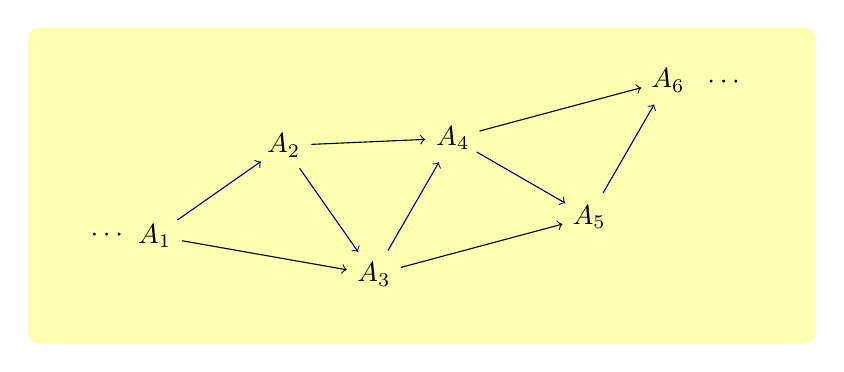
\begin{tikzpicture}
            \fill[draw, Yellow!30, rounded corners]
            (-5, -2) rectangle (5, 2);
            \node at (-4.3,1.5) {$\cc$};
            \pgfmathsetmacro{\r}{2}
    
            \begin{scope}[xshift = -1.25cm, rotate = -10]
                \coordinate (A1) at (-2,-1);
                \pgfmathsetmacro{\x}{-2 + \r*cos(45 )};
                \pgfmathsetmacro{\y}{-1 + \r*sin(45 )};
                \coordinate (A2) at (\x,\y);
                \pgfmathsetmacro{\x}{\x + \r*cos(-45 )};
                \pgfmathsetmacro{\y}{\y + \r*sin(-45 )};
                \coordinate (A3) at (\x,\y);
                \pgfmathsetmacro{\x}{\x + \r*cos(70 )};
                \pgfmathsetmacro{\y}{\y + \r*sin(70 )};
                \coordinate (A4) at (\x,\y);
                \pgfmathsetmacro{\x}{\x + \r*cos(-20 )};
                \pgfmathsetmacro{\y}{\y + \r*sin(-20 )};
                \coordinate (A5) at (\x,\y);
                \pgfmathsetmacro{\x}{\x + \r*cos(70 )};
                \pgfmathsetmacro{\y}{\y + \r*sin(70 )};
                \coordinate (A6) at (\x,\y);
    
                \foreach \n in {1,2,3,4,5,6}{
                    \node at (A\n) {$A_{\n}$};
                }
                \node at ([xshift = -0.6cm, yshift= -0.1cm]A1) {$\cdots$};
                \node at ([xshift = 0.7cm, yshift =0.1cm]A6) {$\cdots$};
    
                \draw[->, shorten >= 10pt, shorten <=10pt, NavyBlue] (A1)--(A2);
                \draw[->, shorten >= 10pt, shorten <=10pt,  NavyBlue] (A2)--(A3);
                \draw[->, shorten >= 10pt, shorten <=10pt,  NavyBlue] (A3)--(A4);
                \draw[->, shorten >= 10pt, shorten <=10pt,  NavyBlue] (A4)--(A5);
                \draw[->, shorten >= 10pt, shorten <=10pt,  NavyBlue] (A5)--(A6);

                \draw[->, shorten >= 10pt, shorten <=10pt] (A1)--(A3);
                \draw[->, shorten >= 10pt, shorten <=10pt] (A2)--(A4);
                \draw[->, shorten >= 10pt, shorten <=10pt] (A3)--(A5);
                \draw[->, shorten >= 10pt, shorten <=10pt] (A4)--(A6);

            \end{scope}
        \end{tikzpicture}
    \end{center}

    Note that in the above picture, we will in general have many possible paths 
    between two different objects. We now face the question: is there a way to 
    organize this data without getting too complicated? 

    To answer that question, we must work with a small category in order 
    to avoid contradictions that arise due to size issues in set theory. 
    With that said, we propose the following definition.         
    
    \begin{definition}
        Let $\cc$ be a small category. For any two objects $A, B$, 
        and for any positive integer $n$, define the \textbf{path set of order} $n$ 
        from $A$ to $B$ as
        \[
            \path^n(A, B)
            = 
            \{ \text{all paths } p: A \to B \text{ of length } n \}.
        \]
        The above definition makes sense, but admittedly it is not illuminating. 
        Is there another perspective we can make from this? 
    \end{definition}

    Yes! Because paths are made of components which are inherently ordered,
    one way to imagine a path is as a tuple 
    $(f_1, \dots, f_n)$ of $n$-morphisms where the codomain of $f_i$ is the domain of $f_{i+1}$.  
    In other words, a path from $A$ to $B$ is an element of 
    \[
        \hom(A, A_1)\times \hom(A_1, A_2)\times \cdots \times \hom(A_n, B).  
    \]
    for some objects $A_1, \dots, A_n$ in $\cc$. Therefore, we can say that 
    \[
        \path^n(A,B)
        =
        \bigcup_{A_1, \dots A_n \in \text{Ob}(\cc)}
        \hom(A, A_1)\times \hom(A_1, A_2)\times \cdots \times \hom(A_n, B).
    \]
    where in the above union we vary across all objects $A_1, \dots, A_n \in \ob(\cc)$. 
    Note that when $n = 1$, we have that $\path^n(A, B) = \hom(A, B)$. In this way, 
    the path set can be thought of as a generalized hom-set. 



    \begin{definition}
        A \textbf{simple diagram} $J$ in a category $\cc$ consists of 
        two distinguished objects 
        $\textcolor{NavyBlue}{A}$ and $\textcolor{Orange}{B}$, referred to as 
        the \textbf{source} and \textbf{target} of $J$, 
        and any finite collection of parallel paths $p_1: A \to B, p_2: A \to B, \dots, p_n: A \to B$ 
        of any length.
    \end{definition}

    Some simple diagrams are pictured below. In the first diagram, the 
    source and targets are $X$ and $Z$; in the second, they are $A$ and $F$; 
    in the third, they are $V$ and $V_7$.
    \begin{center}
        \hspace{1cm}
        \begin{tikzpicture}
            \begin{scope}
                \node at (0,0){
                    \begin{tikzcd}[row sep = 1.4cm, column sep = 0.8cm]
                        & Y \arrow[dr]&\\
                        \textcolor{NavyBlue}{X} \arrow[rr]
                        \arrow[ur]
                        & 
                        &
                        \textcolor{Orange}{Z}
                    \end{tikzcd}
                };
            \end{scope}
            \begin{scope}[xshift =4.2cm]
                \node at (0,0){
                    \begin{tikzcd}[row sep = 1.4cm, column sep = 1cm]
                        \textcolor{NavyBlue}{A} 
                        \arrow[r]
                        \arrow[d] 
                        & 
                        B
                        \arrow[r]
                        \arrow[d] 
                        &
                        C
                        \arrow[d]
                        \\
                        D \arrow[r]
                        & 
                        E
                        \arrow[r]
                        &
                        \textcolor{Orange}{F}
                    \end{tikzcd}  
                };
            \end{scope}
            \begin{scope}[xshift = 10cm, yshift=-1cm]
                \pgfmathsetmacro{\r}{3};
                \node (V) {$\textcolor{NavyBlue}{V}$};
                \foreach \n/\ang in {1/0, 2/30,3/60,4/90,5/120,6/150,7/180}{
                    \pgfmathsetmacro{\x}{\r*cos(\ang)};
                    \pgfmathsetmacro{\y}{\r*sin(\ang)};
                    \coordinate (V_\n) at (\x, \y);
                }
                \foreach \n in {1, 2, ..., 6}{
                    \node at (V_\n) {$V_\n$};
                }
                \node at (V_7) {$\textcolor{Orange}{V_7}$};
                \foreach \n in {1,2, 3, 4, 5, 6,7}{
                    \draw[->, shorten >= 10pt, shorten <=4pt] (V) -- (V_\n);
                }
                \foreach \n/\nn in {2/1,3/2,4/3, 5/4, 6/5,7/6}{
                    \draw[<-, shorten >= 10pt, shorten <=10pt] (V_\n)--(V_\nn);
                }
            \end{scope}
        \end{tikzpicture}
    \end{center}
    In many situations, simple diagrams are what we really care about. This is because 
    often times we have two objects of interests, and we consider many possible paths between 
    them.
    And in those situations, we are generally asking: are all such paths equivalent? 

    This is something high schoolers ask themselves all the time, and a mistake 
    they make all the time. Let $n \ge 2$. Consider the functions
    \begin{itemize}
        \item $e: \mathbb{N} \to \mathbb{N}$ where $f(a) = a^n$ ($e$ for exponent)
        \item $p: \mathbb{N}\times \mathbb{N} \to \mathbb{N}$ where  $f(a,b) = a + b$ ($p$ for plus)
    \end{itemize}
    Often times, they get confused and think that the paths of the diagram below are equivalent.
    \begin{center}
        \begin{tikzcd}[column sep = 1.4cm, row sep = 1.4cm]
            \mathbb{N}\times \mathbb{N}
            \arrow[r, "p"]
            \arrow[d, swap, "{(e, e)}"]
            &
            \mathbb{N}
            \arrow[d, "e"]
            \\
            \mathbb{N}\times \mathbb{N}
            \arrow[r, swap, "p"]
            &
            \mathbb{N}
        \end{tikzcd}
        \hspace{1cm}
        \begin{tikzcd}[column sep = 1.4cm, row sep = 1.4cm]
            (a,b)
            \arrow[r ,maps to]
            \arrow[d, maps to]
            &
            a + b
            \arrow[d, maps to]
            \\
            (a^n, b^n) 
            \arrow[r, maps to]
            &
            a^n + b^n = (a + b)^n 
        \end{tikzcd}
    \end{center}
    Sadly, this equation does not hold generally, and the two paths of the diagram 
    are not equivalent. Thus at this point we introduce terminology for 
    discussing when paths are equivalent.

    \begin{definition}
        Let $J$ be a simple diagram in $\cc$. If every parallel path is equal, then we say
        $J$ \textbf{commutes} and is a \textbf{commutative diagram}. 
    \end{definition}

    At this point, we should note that there is still some work to be done, since 
    of course not all ``diagrams'' that we care about are simple. 
    For example, an extremely important diagram that will 
    eventually become engrained in your brain is pictured below on the left.\footnote{Understanding this diagram right now is not important; there is a lot 
    more stuff one needs to learn before we get into what this means. Long story short, 
    it is the \emph{universal property of a product}.}
    \begin{center}
        \begin{tikzcd}[column sep = 1.4cm, row sep = 1.4cm]
            & Z 
            \arrow[dl, swap, "f"]
            \arrow[dr, "g"]
            \arrow[d, "h"]
            & 
            \\
            X
            &
            \arrow[l, "\pi_1"]
            X \times Y
            \arrow[r, swap, "\pi_2"]
            &
            Y
        \end{tikzcd}
        \hspace{1cm}
        \begin{tikzcd}[column sep = 1.2cm, row sep = 1.4cm]
            & z
            \arrow[dl, maps to]
            \arrow[dr, maps to]
            \arrow[d, maps to]
            & 
            \\
            f(z)
            &
            \arrow[l, "\pi_1"]
            h(z) = (f(z), g(z))
            \arrow[r, swap, "\pi_2"]
            &
            g(z)
        \end{tikzcd}
    \end{center}
    Here, the objects are sets, and the morphisms are functions; the underlying function 
    maps are pictured above on the right. 

    Clearly this diagram is not simple. However, note that it is built from simple 
    diagrams; specifically, the left and right triangles are simple diagrams. 
    At this point, it is clear that the task of rigorously defining the notion of  
    a diagram is reduced to defining what exactly we mean by ``building'' such 
    diagrams.

    {\large \textbf{Exercises}
    \vspace{0.2cm}}
    \begin{itemize}
        \item[1.] Consider a category $\cc$ with objects $A, A_0, \dots, A_n, B, B_0, B_1, \dots, B_m$.
        Let $A_0 = B_0 = A$ and $A_n = B_m = B$, and suppose we have a family of  
        isomorphisms $f_i: A_{i-1} \isomarrow A_i$ and $g_i: B_{i-1} \isomarrow B_i$ as below. 
        \begin{center}
            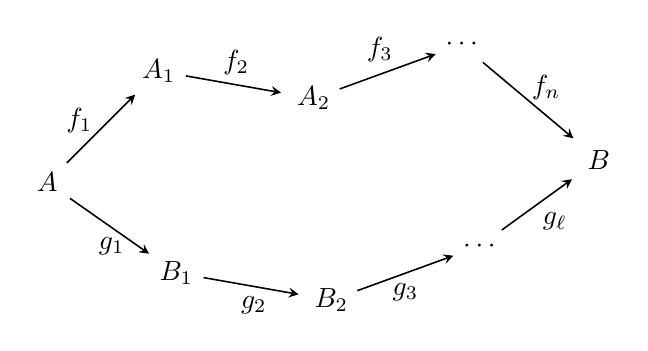
\begin{tikzpicture}[line width = 0.2mm, >=stealth, shorten >= 12pt, shorten <=10pt]
                \draw[->, Black] (0,0) coordinate (a)
                -- node[above, xshift = -0.3cm, yshift = -0.2cm] {$f_1$} ++(45:2) coordinate (b);
                \draw[->, Black,] (b)
                -- node[above] {$f_2$} ++(-10:2) coordinate (c);
                \draw[->, Black, shorten >= 10pt] (c)
                -- node[above, xshift = -0.1cm] {$f_3$} ++(20:2) coordinate (d);
                \draw[->, Black] (d)
                -- node[above, xshift = 0.2cm, yshift = -0.1cm] {$f_n$}++(-40:2.275) coordinate (e);
                \node[] at (a) {$A$};
                \node[] at (b) {$A_1$};
                \node[] at (c) {$A_2$};
                \node[] at (d) {$\cdots$}; 
                \node[] at (e) {$B$};
        
                \draw[->, Black] (0,0)
                -- node[below] {$g_1$}++(-35:2) coordinate (f);
                \draw[->, Black] (f)
                -- node[below] {$g_2$}++(-10:2) coordinate (g);
                \draw[->, Black, shorten >= 10pt] (g)
                -- node[below] {$g_3$}++(20:2) coordinate (h);
                \draw[->, Black] (h)
                -- node[below, xshift = 0.2cm] {$g_{\ell}$} (e);
                \node[] at (f) {$B_1$};
                \node[] at (g) {$B_2$};
                \node[] at (h) {$\cdots$};
            \end{tikzpicture}
        \end{center}
        Suppose we have another object $C$ and isomorphisms $\phi_i: A_i \isomarrow C$,
        $\psi_i: B_i \isomarrow C$ with $\psi_0 = \phi_0$ and $\phi_n = \psi_m$. 
        Prove that if $\phi_{i} \circ f_i = \phi_{i+1}$ 
        and $\psi_{i} \circ g_i = \psi_{i+1}$, then the above diagram is commutative in $\cc$. 
    \end{itemize}








    \newpage
    \section{Functors}
    % Consider the following quote by Saunders Mac Lane: 
    % \begin{center}
    %     \begin{minipage}{0.8\textwidth}
    %         %https://mathoverflow.net/questions/143754/category-was-defined-in-order-to-define-functor-which-was-defined-in-order
    %         As Freyd has observed, "category" has been defined in order to be able to define "functor" and "functor" has been defined in order to be able to define natural transformation
    %     \end{minipage}
    % \end{center}
    At this point, we really have no significant reason to care about categories. 
    They have only so far proved to be an organizatonal tool for concepts of mathematics, 
    but that is about it. In this section, we introduce the abstract notion of a functor
    which is prevalent \emph{everywhere} in mathematics. Functors are ultimately 
    a helpful notion which we care a lot about, but in order to define a functor 
    we first needed to define categories. 
    But as we have defined categories, we move on to defining functors. 
    \begin{definition}
        Let $\cc$ and $\dd$ be categories. A \textbf{(covariant) functor} $F: \cc \to
        \dd$ is a ``mapping'' such that
        \begin{itemize}
            \item[1.] Every $C \in \ob(\cc)$ is assigned uniquely to some
            $F(C) \in \dd$
            \item[2.] Every morphism
            $f: C \to C'$ in $\cc$ is assigned uniquely to some morphism $F(f):
            F(C) \to  F(C')$ in $\dd$ such that 
            \begin{statement}{ProcessBlue!10}
            \begin{align_topbot}
                F(1_C) = 1_{F(C)} \quad\quad F(g \circ f) = F(g) \circ F(f)
            \end{align_topbot}
            \end{statement}
        \end{itemize}
    \end{definition}

    If you have seen a graph homomorphism before, this definition might seem similar. 
    This is no coincidence, and we'll see later on what the relationship between categories 
    and graphs really are. But with that intuition in mind, we can visualize the action of a functor.
    Below we have arbitrary categories $\cc$, $\dd$, and a functor $F: \cc \to \dd$.

    \begin{center}
        \begin{tikzpicture}
            \begin{scope}
                \filldraw[draw, Yellow!30, rounded corners]
                (-3, -2) rectangle (3, 2);
                \node at (-2.5, 1.5) {$\cc$};
                \node at (-2.4, -0.9) {$\cdots$};
                \node at (2.4, -0.9) {$\cdots$};
                \node at (-0.7, 0.9) {$\cdots$};
                \node at (0.7, 0.9) {$\cdots$};

                \node at (0.05, 1.7) {$\vdots$};
                \node at (-1.7, -1.4) {$\vdots$};
                \node at (1.7, -1.4) {$\vdots$};
                \node at (0,0){
                \begin{tikzcd}[row sep = 1.2cm]
                    &
                    A
                    \arrow[dl, swap,  "f"]
                    \arrow[dr, "g\circ f"]
                    & 
                    \\
                    B \arrow[rr, swap, "g"]
                    & & C
                \end{tikzcd}};
            \end{scope}


            \begin{scope}[xshift = 9cm]
                \filldraw[draw, ProcessBlue!10, rounded corners]
                (-4, -2) rectangle (4, 2);
                \node at (-3.3, 1.5) {$\dd$};

                \node at (-3.2, -0.9) {$\cdots$};
                \node at (3.2, -0.9) {$\cdots$};
                \node at (-1, 0.9) {$\cdots$};
                \node at (1, 0.9) {$\cdots$};

                \node at (0, 1.7) {$\vdots$};
                \node at (-2.4, -1.4) {$\vdots$};
                \node at (2.4, -1.4) {$\vdots$};
                \node at (0,0){
                \begin{tikzcd}[row sep = 1.2cm]
                    &
                    F(A)
                    \arrow[dl, swap,  "F(f)"]
                    \arrow[dr, "F(g\circ f)"]
                    & 
                    \\
                    F(B) \arrow[rr, swap, "F(g)"]
                    & & F(C)
                \end{tikzcd}};
            \end{scope}
        \end{tikzpicture}
    \end{center}

    In what follows, we offer some simple and abstract examples that 
    can get us familiar with the behavior of functors. In the next section, 
    we do the opposite, and instead use our abstract understanding of functors to 
    witness functors in real mathematical constructions\footnote{I chose to separate this section and the 
    next to ease the learning curve for functors; both perspectives are necessary for true understanding 
    of a functor.}.  

    \begin{example}
        Denote $\bm{1}$ as the category with one 
        object $\bullet$ and one identity morphism $1_\bullet: \bullet \to \bullet$. 
        Then for any category $\cc$, there exists 
        a unique functor $F: \cc \to \bm{1}$ which sends every object to $\bullet$ 
        and every morphism to $1_\bullet$. 

        Conversely, there are many functors $F: \bm{1} \to \bm{\cc}$. Since we only have 
        $F(\bullet) = A$ for some $A \in \cc$, and $F(1_\bullet) = 1_A$, we see that this functor 
        simply picks out one element of $\cc$. So these functors are in correspondence 
        with the objects of $\cc$; the picture below may help.

        \begin{center}
            \begin{tikzpicture}
                \begin{scope}
                    \fill[draw, Yellow!30, rounded corners]
                    (-2.5, -1.2) rectangle (2.5, 1.2);
                    \node at (-2,0.7) {$\bm{1}$};
                    \node at (0,0){
                        \begin{tikzcd}
                            \bullet
                            \arrow[out=120,in=60,looseness=3,loop, "1_{\bullet}"]
                        \end{tikzcd}
                    };
                \end{scope}
                \begin{scope}[xshift=7cm]
                    \node at (-2.5,0.7) {$\cc$};
        
                    \node at (0,-0.8) {$\vdots$};
                    \node at (-0.8, -0.4) {$\cdots$};
                    \node at (0.8, -0.4) {$\cdots$};
                    \fill[draw, ProcessBlue!30, rounded corners, opacity = 0.3]
                    (-3, -1.2) rectangle (3, 1.2);
                    \node at (0,0.25){
                        \begin{tikzcd}
                            A
                            \arrow[out=120,in=60,looseness=3,loop, "1_A"]
                        \end{tikzcd}
                    };
                \end{scope}
            \end{tikzpicture}
        \end{center}
    \end{example}

    \begin{example}
        Let $\bm{2}$ be the category with two objects $\textcolor{Blue}{\bullet}$ 
        and $\textcolor{Orange}{\bullet}$ with one nontrivial $f: \textcolor{Blue}{\bullet} \to \textcolor{Orange}{\bullet}$. 
        The category can be pictured as below. 
        \begin{center}
            \begin{tikzpicture}
                \fill[draw, Yellow!30, rounded corners]
                (-2.5, -1.2) rectangle (2.5, 1);
                \node at (-2,0.6) {$\bm{2}$};
                \node at (0,0){
                    \begin{tikzcd}
                        \textcolor{Blue}{\bullet}
                        \arrow[out=120,in=60,looseness=3,loop, "1_{\textcolor{Blue}{\bullet}}"]
                        \arrow[r, "f"]
                        &
                        \textcolor{Orange}{\bullet}
                        \arrow[out=120,in=60,looseness=3,loop, "1_{\textcolor{Orange}{\bullet}}"]
                    \end{tikzcd}
                };
            \end{tikzpicture}
        \end{center}
        Suppose now that $\cc$ is an arbitrary category, and that we 
        have a functor $F: \bm{2} \to \cc$. Then note that $F(\textcolor{Blue}{\bullet}) = A$ 
        and $F(\textcolor{Orange}{\bullet}) = B$ for some objects $A, B \in \cc$. Hence we have that 
        $F(f) = \phi: A \to B$ for some $\phi \in \cc$. Below we have the functor pictured. 
        \begin{center}
            \begin{tikzpicture}
                \begin{scope}
                    \fill[draw, Yellow!30, rounded corners]
                    (-2.5, -1.2) rectangle (2.5, 1.2);
                    \node at (-2,0.7) {$\bm{2}$};
                    \node at (0,0){
                        \begin{tikzcd}
                            \textcolor{Blue}{\bullet}
                            % \arrow[out=120,in=60,looseness=3,loop, "1_{\textcolor{Blue}{\bullet}}"]
                            \arrow[r, "f"]
                            &
                            \textcolor{Orange}{\bullet}
                            % \arrow[out=120,in=60,looseness=3,loop, "1_{\textcolor{Orange}{\bullet}}"]
                        \end{tikzcd}
                    };
                \end{scope}
                \begin{scope}[xshift=7cm]
                    \node at (-2.5,0.7) {$\cc$};
                    \node at (-0.8,0.7) {$\vdots$};
                    \node at (-0.8,-0.6) {$\vdots$};
                    \node at (0.8,0.7) {$\vdots$};
                    \node at (0.8,-0.6) {$\vdots$};
                    \node at (-1.4, -0.05) {$\cdots$};
                    \node at (1.4, -0.05) {$\cdots$};
                    \fill[draw, ProcessBlue!30, rounded corners, opacity = 0.3]
                    (-3, -1.2) rectangle (3, 1.2);
                    \node at (0,0){
                        \begin{tikzcd}
                            \textcolor{Blue}{A}
                            \arrow[r, "\phi"]
                            &
                            \textcolor{Orange}{B}
                        \end{tikzcd}
                    };
                \end{scope}
            \end{tikzpicture}
        \end{center}
        Note we suppressed the identity morphisms. 
        Therefore, we see that this functor simply picks out morphisms $\phi: A \to B$ in $\cc$. 
        So we can say that functors $F: \bm{2} \to \cc$ are in correspondence with the 
        morphisms of $\cc$. 
    \end{example}

    Consider the very first figure of this section, Figure \ref{figure:functor_def}.
    In that image we saw three objects $A,B,C$ get sent to $F(A),F(B),F(C)$. However, the 
    original commutative diagram involving $f, g$ and $g \circ f$ was translated into another 
    commutative diagram in $\dd$ involving $F(f), F(g)$ and $F(g \circ f)$. 
    This is because of the critical property $F(g \circ f) = F(g) \circ F(f)$ 
    given by a functor. In fact, any commutative diagram translates to a commutative 
    diagram under a functor. 

    \begin{proposition}
        Let $\cc, \dd$ be categories with $F: \cc \to \dd$ a functor. 
        Suppose $J$ be a commutative diagram in $\cc$. Then the diagram obtained 
        from the image of  
        $J$ under $F$, which we denote as $F(J)$, is commutative in $\dd$.
    \end{proposition}

    \begin{prf}
        It suffices to prove that,
        for any complete subdiagram $J'$ of $J$ involving any 
        two distinct paths
        \[
            p = f_n \circ f_{n-1} \circ \cdots \circ f_1 \qquad q = g_m \circ g_{m-1} \circ \cdots \circ g_1
        \]
        in $J$, we have that $F(J')$ is commutative in $\dd$. But this immediate. 
        Since $J'$ is commutative in $\cc$, we have that $p = q$. Hence 
        we see that 
        \[
            F(p) = F(q) \implies F(f_n) \circ F(f_{n-1}) \cdots F(f_1) = F(g_m) \circ F(g_{m-1}) \circ \cdots \circ F(g_1).
        \]
        by repeatedly applying the composition property of a functor.
        Hence $F(J')$ is commutative of $J$. Since 
    \end{prf}

    Finally, before we move onto the next section and introduce various examples of 
    functors across mathematics, we introduce one of the most important 
    functors in basic category theory. 

    \begin{example}
        Let $\cc$ be a locally small category. Then for every object $A$, 
        we obtain the \textbf{covariant hom-functor} denoted as 
        \[
            \hom_{\cc}(A, -): \cc \to \Set.
        \]
        where on objects $C \mapsto \hom_{\cc}(A, C)$ and on morphisms 
        $(\phi: C \to C') \mapsto \phi^*: \hom_{\cc}(A, C) \to \hom_{\cc}(A, C'))$
        where  $\phi^*$ is a function defined pointwise as 
        \[
            \phi^*(f: A \to C) = \phi \circ f: A \to C'.
        \]
        Such a functor is naturally of interest in mathematics since it is often 
        of interetst to consider the hom set $\hom_{\cc}(A, B)$ for some objects $A, B$ 
        in a category $\cc$, as it is usually the case that this set contains extra structure.
        For example, within topology this set is always a topological space, since 
        families of continuous functions can be endowed with the compact open topology.
        In the setting of abelian groups, this set also forms an abelian group. Much of category 
        theory can actually be done by simply ``enriching'' hom sets of a category with 
        some extra structure; this is the object of enriched category theory, which we'll introduce later.

        This functor in general also exhibits nice properites. For example, 
        let $R$ be a ring. Then the sequence below
        \begin{center}
            \begin{tikzcd}
                0 \arrow[r]
                &
                M_1 \arrow[r, "\phi"]
                &
                M \arrow[r, "\psi"]
                &
                M_2
            \end{tikzcd}
        \end{center}
        is exact if and only if, for every $R$-module $N$, the sequence 
        \begin{center}
            \begin{tikzcd}
                0 \arrow[r]
                &
                \hom(N, M_1) \arrow[r, "\phi^*"]
                &
                \hom(N, M) \arrow[r, "\psi^*"]
                &
                \hom(N, M_2)
            \end{tikzcd}
        \end{center}
        is exact. This result even extends to split short exact sequences. We 
        also have that for $R$-modules $N$, $M_1, M_2$ that 
        \[
            \hom(N, M_1\oplus M_2)\cong \hom(N, M_1)\oplus \hom(N, M_2).
        \]
        This result also holds for arbitrary direct sums,
        so that the hom functor distributes over all direct sums.
        Even better, we cannot forget that the hom-functor exhibits the 
        \textbf{tensor-hom adjunction} which states that for
        $R$-modules $N, M_1, M_2$ 
        \[
            \hom(N \otimes M_1, M_2) \cong \hom(N, \hom(M_1, M_2)).
        \]
        More is to be said about this property; we'll later 
        see that this is an example of an \emph{adjunction}.


    \end{example}





                        



    \newpage
    \section{Examples and Nonexamples of Functors}
    Functors were not defined out of arbitrary interest. The definition of a functor 
    was motivated by constructions that were seen in mathematics
    (unlike constructions in say, number theory, which 
    are interesting in their own right). 
    Thus in this section, we include a wide variety of different constructions in 
    in different areas of mathematics which all fit the definition of a functor. 
    We present examples 
    from algebraic topology, differential geometry, topology, algebraic geometry, 
    abstract algebra and set theory.

    In short, this section is due to the fact that the only way to really understand what a functor does is to realize 
    the definition \emph{with examples}.  It's not necessarily important to understand \emph{all} 
    the examples, if for instance you have never worked with differential geometry, 
    but it would be good to get a few of them. What is more important is 
    witnessing how such a simple definition can be so versatile and prevalent
    in seemingly different fields of mathematics; thus, what is important is 
    witnessing the flexibility of functors (in addition to filling in the details of 
    the examples and doing the exercises at the end).
    \\

    % {\large\noindent \textbf{Thin Categories.}\par}

    % \begin{example}
    %     Consider the thin category $\mathbb{N} = \{0, 1, 2, \dots \}$ regarded 
    %     as a preorder. Then multiplication and addition correspond to functors:
    %     \begin{align*}
    %         \cdot&: \mathbb{N}\times \mathbb{N} \to \mathbb{N} \qquad (n, m) \mapsto n \cdot m\\
    %         +&: \mathbb{N}\times \mathbb{N} \to \mathbb{N} \qquad (n, m) \mapsto n + m.
    %     \end{align*}
    %     This is simply due to the following simple observation. If 
    %     $n \le n'$ and $m \le m'$, then we have one morphism $(n, m) \to (n', m')$ in $\mathbb{N} \times \mathbb{N}$. 
    %     Furthemore, $n \cdot m \le n' \cdot m'$ and $n +m \le n' + m'$. Hence we see that 
    %     there is one morphism  $n\cdot m \to n' \cdot m'$ and $n +m \to n' + m'$. 

    %     Note however that this does not generalize to $\mathbb{Z}$. In this situation, 
    %     multiplication fails to be a functor. 
    % \end{example}



    {\large\noindent \textbf{Algebraic Geometry.}\par}

    \begin{example}
        In algebraic geometry, it is often of interest to construct the \textbf{affine $n$-space}
        $A^n(k)$ of a field $k$. Usually, $k$ is an algebraically closed field, but it doesn't have to be.
        \[
            A^n(k) = \{(a_0, \dots, a_{n-1}) \mid a_i \in k \}.
        \]  
        For example, when $k = \rr$, we have that $A^n(k) = \rr^n$. 
        Moreover, we claim that we have a functor $A^n(-): \fld \to \Set$.
        To see this, we need to figure out where $A^n(-)$ sends objects and morphisms.
        
        We can first observe that $A^n(-)$ sends fields $k$ to sets $A^n(k)$.
        Secondly, we can observe that for a field homomorphism $\phi: k \to k'$,    
        we can define the function $A^n(\phi): A^n(k) \to A^n(k')$ where
        for each $(a_1, \dots, a_n) \in A^n(k)$ we have that
        \[
            A^n(\phi)(a_0, \dots, a_{n-1}) = (\phi(a_0), \dots,  \phi(a_{n-1})).
        \] 
        The reader can show that this satisfies the rest of the axioms of a functor. Overall, 
        we can say that we have a functor 
        \[
            A^n(-): \fld \to \Set.  
        \]
    \end{example}

    \begin{example}
        Once the affine $n$-space is defined, the next step in algebraic geometry is to construct 
        the \textbf{projective space} $P^n(k)$ for a field $k$. To define this, we first 
        define an equivalence relation on $A^{n+1}(k)$. We say 
        \[
            (a_0, \dots,  a_n) \sim (b_0, \dots, b_n) \text{ if there is a nonnzero } \lambda \in k \text{ such that } a_i = \lambda b_i.
        \]  
        This defines an equivalence relation on the points of $A^n(k)$. Geometrically, this equivalence relation 
        says two points are equivalent whenever they lie on the same line passing through the origin.
        With this equivalence relation, we then define
        \[
            P^n(k) = A^{n+1}/\sim = \Big\{[(a_0, \dots, a_n)] \mid (a_0, \dots, a_n) \in A^{n+1}(k)\Big\}.
        \]
        Hence we see that $P^n(k)$ is the set of equivalence classes under this equivalence relation. Similar to 
        the previous example, this construction is also functorial. Consider a field homomorphism $\phi: k \to k'$. Then we 
        define the function $P^n(\phi): P^n(k) \to P^n(k')$ where 
        \[
            P^n(\phi)([a_0, \dots, a_n]) = [(\phi(a_0), \dots, \phi(a_n))].           
        \]
        However, when defining functions on a set of equivalence classes, we need to be careful. 
        It's possible that the function could send equivalent objects to different things, so that such 
        a fuction would not be well-defined. In this case, the above function is in fact well-defined. 
        This is because $\phi(\lambda a_i)  =\phi(\lambda) \phi(a_i)$ for any $i = 0, 1, \dots, n$. 
        Therefore we can state that we have a functor 
        \[
            P^n(-): \fld \to \Set.  
        \]
    \end{example}
    \vspace{0.5cm}  

    {\large\noindent \textbf{Algebraic Topology.}\par}

    \begin{example}
        An important example of a
        functor arises in homology theory. For example, in singular homology
        theory, one considers a topological space $X$ and associates this 
        with its $n$-th homology group.
        \[
            X \mapsto H_n(X)
        \]
        In a typical 
        topology course, one then proves that if $f: X \to Y$ is a continuous 
        mapping between topological spaces, then $f$ induces a group homomorphism 
        \[
            H_n(f): H_n(X) \to H_n(Y) 
        \]
        in such a way that for a second mapping $g: Y \to Z$, $H_n(g \circ f) 
        = H_n(g) \circ H_n(f)$ for all $n$. Finally, we also know that 
        $H_n(1_X) = 1_{H_n(X)}$.
        Therefore, what we see is that this process can be cast into the language 
        of category theory, so that we may define a \textbf{singular 
        homology functor}
        \[
            H_n: \top \to \ab
        \]
        since this functorial process sends topological spaces in $\top$
        to abelian groups in $\ab$.
    \end{example}

    \begin{example}\label{example:fundamental_group}
        Another example from algebraic topology can be
        realized from the \textbf{fundamental group}
        \[
            \pi_1(X, x_0) = \{[x] \mid x \in X\}
        \] 
        with $x_0 \in X$, and 
        where $[x]$ is the equivalence class of loops based at $x_0$, subject 
        to the homotopy equivalence 
        relation. First observe that $X \mapsto \pi_1(X)$ is in fact a mapping 
        of objects between $\top^*$ and $\grp$. Second, 
        observe that if $f: X \to Y$ is a continuous function, then 
        we can define a group homomorphism 
        \[
            \pi_1(f): \pi_1(X) \to \pi_1(Y) \qquad [x] \mapsto [f(x)].
        \]
        Note that this is well defined since if $x \sim x'$ then 
        there is a homotopy relation $H: X \times [0, 1] \to Y$. However, 
        $f \circ H$ is also another homotopy relation that establishes that 
        $f(x) \sim f(x')$; hence our group homomorphism is well defined. 
        
        Moreover, if $f: X \to Y$ and $g:Y \to Z$ are continuous, then 
        we can check that $\pi_1(g \circ f) = \pi_1(g) \circ \pi_1(f)$;
        if $[\alpha] \in \pi_1(X, x_0)$,
        then
        \[
            (g \circ f)_*([\alpha]) = [(g \circ f) \circ \alpha] 
            = [g \circ (f \circ \alpha)]
            = g_*([f_*([\alpha])]) = g_* \circ f_*([\alpha]) 
        \]
        so that $(g \circ f)_* = g_*f_*$. Finally, we 
        can examine how the identity map $1_X$ on a topological 
        space acts on an element $[\alpha] \in \pi_1(X, x_0)$:
        \[
            id_*([\alpha]) = [id \circ \alpha] = [\alpha].
        \]
        so that it is sent to the identity homomorphism. All together, this allows 
        us to conclude that this process is entirely functorial, so we may summarize our 
        results by stating that 
        \[
            \pi_1: \top^* \to \grp   
        \]
        is a functor.
    \end{example}

    We now present two examples from differential geometry, which aren't traditionally 
    presented as examples of functors but are nevertheless interesting in their 
    own right. 
    \vspace{0.5cm}

    {\large\noindent \textbf{Differential Geometry.}\par}
    \begin{example}
        Let $M^n$ be a differentiable manifold of dimension $n$. In general, this 
        means that there exists
        a family of open sets $U_\alpha \subset \rr^n$ and injective 
        mappings $\bm{x}_\alpha: U_\alpha \to M$ for $\alpha \in \lambda$, $\lambda$ an indexing 
        set, with the mappings subject to various conditions\footnote{There isn't 
        a universally agreed upon set of conditions, and we won't really need to worry about 
        them here. If the reader likes, they can consult Do Carmo's \emph{Riemannian Geometry}, 
        which is, and has been for a long time, the go-to differential geometry text.
        }. 
        Recall from differential 
        geometry that we can associate each point $p \in M^n$ with its \textbf{tangent space}
        $T_p(M)$, in the following manner. 
        
        Suppose for $\alpha' \in \lambda$ we have that 
        $\bm{x}_{\alpha}: U_{\alpha} \to M$ is a mapping whose image contains $p$ (such an $\alpha'$ must exist).
        Then $T_p(M)$ has a basis 
        \[
            \left\{ \frac{\partial}{\partial x_1}, \frac{\partial}{\partial x_2}, \dots, \frac{\partial}{\partial x_n} \right\}
        \]
        where $\displaystyle \frac{\partial}{\partial x_i}$ is the tangent vector of the map 
        $\bm{c}_i: U \to M$, which simply sends $(0, \dots ,0, x_i, 0, \dots, 0)$. 

        Now suppose $\phi: M_1^n \to M_2^m$ is a differentiable mapping. Recall 
        that the \textbf{differential} of $\phi$ establishes a 
        linear transformation between the vector spaces: 
        \[
            d\phi_p: T: M^n_1 \to T_{\phi(p)}M^m_2.
        \]  
        Consider the category $\textbf{DMan}^*$
        whose objects are pairs $(M^n, p)$ with $M^n$ a differentiable manifold and 
        $p \in M^n$. The morphism are 
        $(\phi, p): (M_1^n,p) \to (M_2^m, q)$ with $\phi: M_1^n \to M_2^m$ a differentiable 
        map and $\phi(p) = q$. 
        Then this process may be summarized as a functor 
        $T_p: \textbf{DMan}_n^* \to \vect_{\rr}$ where 
        \begin{gather*}
            T:(M, p) = T_p(M)\\
            T(\phi: (M_1^n,p) \to (M_2^m, \phi(p)) ) 
            = d\phi_{p}: T_p(M) \to T_{\phi(p)}M_2^m
        \end{gather*}
        One can show that the identity map is sent to the identity linear transformation 
        on $T_p(M)$ and that the differential respects composition, so that 
        that the association of a manifold $M$ (with a specified point $p \in M$) 
        to its tangent space $T_p(M)$ gives rise to a functor
        \[
            T_p: \textbf{DMan}^* \to \vect_{\rr}.
        \]
    \end{example}\label{example:manifold_tangent_planeone}

    \begin{example}
        Consider again a differentiable manifold $M^n$ of dimension $n$. Recall that 
        we may consider the \textbf{tangent bundle} $TM$ of $M$, which is the set 
        \[
            TM = \{(p, v) \mid p \in M^n \text{ and } v \in T_p(M)\}.
        \]
        The set $TM$ simply pairs each point $p \in M^n$ with its tangent space $T_p(M)$. 
        However, $TM$ is more than such a set; it inherits the structure of a differentiable manifold 
        from $M$ as well. In fact, it is a manifold of dimension $2n$. 

        Now suppose we have a differentiable mapping $\phi: M_1^n \to M_2^m$. Then 
        this induces a mapping 
        \begin{gather*}
            (\phi, d\phi): TM_1^{2n} \to TM_2^{2m}\\
            (\phi, d\phi)(p, v) = (\phi(p), d\phi_p(v)).
        \end{gather*}
        One can show that $(\phi, d\phi): TM_1^{2n} \to TM_2^{2m}$ is a differentiable mapping 
        between manifolds\footnote{I wanted to show this here, 
        but it turned out to be just tedious definition-checking, so I don't think it's appropriate 
        to include here (\textcolor{Red}{perhaps I could make/put it in an appendix...})} 
        At this point we may guess that we have a functor 
        $TB: \textbf{DMan} \to \textbf{DMan}$ (``$TB$'' for ``tangent  bundle'') 
        where 
        \begin{gather*}
            TB(M^n) = TM\\
            TB(\phi: M_1^n \to M_2^m) = (\phi, d\phi): TM_1^{2n} \to TM_2^{2m}.
        \end{gather*}        
        To check this, we first observe that $TB(1_{M^n}) = 1_{TM^{2n}}$.
        Next, suppose $\phi: M_1^n \to M_2^m$ and $\psi: M_2^m \to M_3^p$, 
        and observe that 
        \[
            TB(\psi \circ \phi)
            = 
            (\psi \circ \phi, d_{\psi \circ \phi})
            =
            (\psi, d_{\psi}) \circ (\phi, d_{\phi})
            =
            TB(\psi) \circ TB(\phi).
        \]
        Note that above in the second step, we used the fact that 
        $d_{\psi \circ \phi} = d_{\psi} \circ d_{\phi}$, which we know is true from 
        the previous example. As $TB$ respects the identity and composition, we see that we 
        do in fact have a functor 
        \[
            T: \textbf{DMan} \to \textbf{DMan}  
        \]
        as desired.
    \end{example}

    \vspace{0.5cm}
    {\large\noindent \textbf{Topology.}\par}

    \begin{example}
        Let $X$ be a set. Recall that we can turn $X$ into a topological space 
        $(X,\tau_d)$, where $\tau^{(X)}_{d}$ is the discrete topology, so that every subset of 
        $X$ is an open set. We claim that this process is functorial, so that we 
        have a functor
        \[
            D: \Set \to \top.
        \]
        This is because any function $f: X \to Y$ extends 
        to a continuous function $f: (X, \tau^{(X)}_{D}) \to (Y, \tau^{(Y)}_D)$ 
        (hopefully the abuse of notation in $f$ is forgivable here).
        Hence this defines a functor, although in a simpler way than we've seen in the 
        previous examples. 
    \end{example}
    
    \begin{example}
        Let $(X, \tau)$ be a topological space and consider any $x_0 \in X$. 
        Then $(X, x_0)$ forms an element of $\top^*$.  With such a space, we can 
        consider the \textbf{loop space} of $(X, x_0)$ defined to be 
        \[
            \Omega(X) = \{\phi: S^1 \to X \mid \phi \text{ is continuous and } \phi(0) = x_0\}. 
        \]
        Here $S^1$ is the circle. 
        As this consists of a family of continuous functions between two topological spaces, 
        it can be endowed with the Compact Open topology to turn it into a topological space as well.
        Hence we claim we have a functor 
        \[
            \Omega: \top^* \to \top.
        \]
        To see this, one needs to first consider a morphism in $\top^*$, which 
        in this case is continuous function $f: (X, x_0) \to (Y, y_0)$  such that 
        $f(x_0 )= y_0$. This must then correspond with a continuous function 
        $\Omega(f): \Omega(X) \to \Omega(Y)$. We can define this function 
        pointwise: for each continuous $\phi: S^1 \to X$ such that $\phi(0) = x_0$, we have that 
        $\Omega(f)(\phi) = f \circ \phi: S_1 \to Y$. In this case we see that $(f \circ \phi)(0) = y_0$, 
        and is a continuous function, so it is well-defined. 

        This example can be further generalized to higher loop spaces which consider continuous 
        functions $\phi: S^n \to X$, rather than just having $n = 1$. 
    \end{example}

    \vspace{0.5cm}

    {\large\noindent \textbf{Algebras, Rings, Groups.}\par}
    \begin{example}
        Recall that a \textbf{Lie Algebra} $\mathfrak{g}$ is a vector space 
        $\mathfrak{g}$ (over a field $k$), equipped with a bilinear operation 
        $[-, -]: \mathfrak{g}\times \mathfrak{g} \to \mathfrak{g}$
        such that 
        \begin{itemize}
            \item[1.] $[x, y] = -[y, x]$
            \item[2.] $[x, [y, z]] + [y, [z, x]] + [z, [x,y]] = 0$. 
        \end{itemize}
        Condition (2) is referred to as the \textbf{Jacobi identity}, and many 
        familiar operations on vector spaces satisfy (1) and (2). For example, the cross 
        product on vector spaces in $\rr^3$ satisfy these properties. 

        Consider an associative algebra $A$ over a field $k$ with (associative); recall 
        that this too has a bilinear operation $\cdot: A \times A \to A$ with unit $e \in A$. 
        Then we can use $A$ to create a Lie algebra $L(A)$, whose (1) underlying vector 
        space is $A$ and (2) whose bilinear operation is $[a, b] = a \cdot b - b\cdot a$. 

        Now suppose $\phi: A \to A'$ is a morphism of algebras. Then we can associate 
        both $A, A'$ with their Lie algebras $L(A), L(A')$. Further, we can construct a Lie 
        Algebra morphism $L(\phi): L(A) \to L(A')$, using $\phi$, by setting 
        $L(\phi)(a) = \phi(a)$. This is a morphism of Lie algebras since 
        \[
            [\phi(a), \phi(b)] = \phi(a)\phi(b) - \phi(b)\phi(a) = \phi(ab - ba) = \phi([a, b]).
        \]
        One can then check that $L(1_A) = 1_{L(A)}$ and $L(\phi \circ \psi) = L(\phi)\circ L(\psi)$, so 
        that what we have is a functor 
        \[
            L: \textbf{Alg} \to \textbf{LieAlg}            
        \]
        which associates each associative algebra with its Lie algebra structure.
    \end{example}

    \begin{example}
        Let $R$ be a commutative ring. Recall that
        $\spec(R)$ is the set of all prime ideals of $R$. In addition, recall
        that if $\phi: R \to S$ is a ring homomorphism and  
        if $P$ is a prime ideal of $S$, then $\phi^{-1}(P)$ is also a prime 
        ideal in $R$.
        This then allows us to define a functor 
        \[
            \textbf{Spec}: \ring \to \Set
        \]
        where on objects $R \mapsto \spec(R)$ and on morphisms 
        $\phi: R \to S \mapsto \phi^*: \spec(S) \to \spec(R)$ where 
        $\phi^{*}(P) = \phi^{-1}(P)$.

        However, we can go even deeper than this. Recall from algebraic 
        geometry that $\spec(R)$ can be turned into a topological space, 
        using the Zariski topology. However, because 
        $\phi^{-1}(P)$ is a prime ideal whenever $P$ is, we see that $\phi^*: 
        \spec(S) \to \spec(R)$ is actually a continuous function between 
        the topological spaces. Hence we can view this 
        as a functor 
        \[
            \textbf{Spec}: \ring \to \top.
        \] 
        Usually this is phrased more naturally as a functor 
        $\textbf{Spec}: \ring \to \textbf{Sch}$
        where $\textbf{Sch}$ is the category of schemes; this is simply 
        because schemes are isomorphic to $\spec(R)$ for some $R$.
    \end{example}

    \begin{example}\label{example:group_ring_functor}
        Let $G$ be a group, and $R$ be a ring with identity. Recall 
        from ring theory that we can form the \textbf{group ring}
        \[
            R[G] = \left\{ \sum_{g \in G}a_gg\mid a_g \in R, \text{ all but finitely many } a_g = 0 \right\}.
        \]
        Thus the elements are finite sums, but we have possibly infinitely many ways 
        of adding them. Now 
        for two elements $\displaystyle \alpha = \sum_{g \in G}a_kg$ and 
        $\displaystyle \beta = \sum_{g \in G}b_gg$, we define ring addition and multiplication 
        as 
        \[
            \alpha + \beta = \sum_{g \in G}(a_k + b_k)g
            \qquad 
            \alpha \cdot \beta 
            = 
            \sum_{g \in G}\sum_{g_1 \cdot g_2 = g}(a_{g_1}b_{g_2})g.
        \]
        Now suppose $\phi: G \to H$ is any group homomorphism.
        With that said, we claim that $\phi$ induces a
        natural ring homomorphism $\phi^{*}: R[G] \to R[H]$
        between the group rings, where 
        \[
            \sum_{g\in G}a_gg \mapsto \sum_{g \in G}a_g \phi(g). 
        \]
        Clearly this is linear and preserves scaling; less obvious is if 
        this behaves on multiplication, although we check that below.
        If $\alpha, \beta$ defined as above then 
        \[
            \phi^*( \alpha \cdot \beta )
            =
            \phi^*\left( \sum_{g \in G}\sum_{g_1 \cdot g_2 = g}(a_{g_1}b_{g_2})g \right)
            =
            \sum_{g \in G}\sum_{g_1 \cdot g_2 = g}(a_{g_1}b_{g_2})\phi(g)
            =
            \sum_{g \in G}a_g\phi(g)\cdot
            \sum_{g \in G}b_g\phi(g)
            =
            \phi^*(\alpha)\cdot\phi^*(\beta).
        \]
        Hence we see that $\phi^*$ is a ring homomorphism. Therefore, 
        what we have on our hands is a functor 
        \[
            R[-]: \grp \to \ring  
        \]
        Possibly, your brain may wonder: it looks like we have an assignment 
        of rings to \emph{functors}. 
        \[
            R \mapsto R[-]: \grp \to \ring.
        \]
        Perhaps this process is functorial? The answer is yes, although 
        at the moment we don't have the necessary language to describe it; 
        we will go over this when we introduce \emph{functor categories}.
    \end{example}
    \vspace{0.5cm}

    {\large\noindent \textbf{Set Theory}\par}
    \begin{example}
        Consider the power set $\mathcal{P}(X)$ on a set $X$.
        Then we can create a functor $\mathcal{P}: \Set \to
        \Set$ as follows. 
        
        Observe that for any set $X$, $\mathcal{P}(X)$ is of course
        another set. Therefore objects of $\Set$ are sent to
        $\Set$, as we claim. 

        Now let $f: X \to Y$ be a function between two sets $X$ and
        $Y$. Then we define $\mathcal{P}(f) : \mathcal{P}(X) \to
        \mathcal{P}(Y)$ to be the function where 
        \[
            P(f)(S) = \{f(x) \mid x \in S\}.
        \]
        which is clearly in $\mathcal{P}(Y)$.
        Now we must show that this function
        respects identity and composition properties.
        \begin{description}
            \item[Identity.] Consider the identity function 
            $\id_X: X \to X$ on a set $X$. 
            Then observe that for any $S \in \mathcal{P}X$, we have that  
            \[
                \mathcal{P}(\id_X)(S) 
                =
                \{\id_X(x) \mid x \in X\} = S.
            \] 
            Therefore, $\mathcal{P}(\id_X) = 1_{\mathcal{P}X}$ so
            that $\mathcal{P}$ respects identities. 

            \item[Composition.] Let $X, Y, Z$ be sets and $f: X \to Y$
            and $g: Y \to Z$ be functions. Let $S \in \mathcal{P}(X)$.
            Observe that 
            \begin{align*}
                \mathcal{P}(g \circ f)(S) 
                &= \{(g \circ f)(x) \mid x \in S \}\\
                &= \{ g(f(x)) \mid x \in S \}\\
                &= \{ g(y) \mid y = f(x) \text{ and } x \in S\}
                &= \mathcal{P}(g)(\{f(x) \mid x \in S\})\\
                &= \mathcal{P}(g)( \mathcal{P}(f)(S))\\
                &= (\mathcal{P}(g) \circ \mathcal{P}(f)) (S).
            \end{align*}
            Therefore we see that $\mathcal{P}(g \circ f) =
            \mathcal{P}(g) \circ \mathcal{P}(f),$ so that
            $\mathcal{P}$ describes a functor from $\Set$ to $\Set$.
        \end{description}
    \end{example}

    As we just encountered a mass of different examples of functors from 
    different fields, one might wonder: are there other mathematical constructions 
    which simply do not behave exactly as a functor? The answer is yes, although 
    finding these examples is a bit tricky. The following is a well-known 
    example, while the one after is one I haven't seen presented elsewhere.
    \vspace{0.5cm}

    {\large\noindent \textbf{Non-functor Examples.}\par}
    
    \begin{example}
        Recall from group theory that, with every group $G$, 
        there is an associated subgroup of $G$ called the center:
        \[
            Z(G) = \{ z \in G \mid zg = gz \text{ for all } g \in G\}.
        \]
        By definition, $Z(G)$ is an abelian group. As every group $G$ may be 
        associated with an abelian group $Z(G)$, one might expect that this 
        process is functorial. One might prematurely denote this as
        \[
            Z: \grp \to \ab.
        \]
        However, this is not a functor, as an issue arises with the morphisms. 
        Consider a group homomorphism $\phi: G \to H$. Then for this to be a functor, 
        we'd naturally desire a group homomorphism $Z(\phi): Z(G) \to Z(H)$ between 
        the abelian groups. The only issue is that there is no consistent way to 
        define such a morphism from $\phi$. The most natural way we would attempt  
        to achieve this is by considering the restriction, but in general 
        $\phi\big|_{Z(G)}: G \to H$ does not map into $Z(H)$. 
        For example, consider the \textbf{Heisenberg Group}
        \[
            H_3(R)
            = 
            \left\{
            \begin{pmatrix}
                1 & a & b\\
                0 & 1 & c\\
                0 & 0 & 1 
            \end{pmatrix}
            \Bigg|
            a,b,c \in R
            \right\}
        \]
        where $R$ is a commutative ring with identity. Observe that 
        we can create an inclusion group homomorphism $i: H_3(R) \to \text{GL}_3(R)$. 
        One can show that 
        \[
            Z(H_3(R)) = 
            \left\{
                \begin{pmatrix}
                    1 & 0 & a\\
                    0 & 1 & 0\\
                    0 & 0 & 1 
                \end{pmatrix}
                \Bigg|
                a \in R
            \right\}
            \qquad 
            Z(\text{GL}_3(R))
            =
            \left\{  
                \begin{pmatrix}
                    a & 0 & 0\\
                    0 & a & 0\\
                    0 & 0 & a 
                \end{pmatrix}
                \Bigg|
                a \in R 
            \right\}.
        \]
        Hence restricting the inclusion $i: H_3(R) \to \text{GL}_3(R)$ 
        to $Z(H_3(R))$ results in a group homomorphism that 
        does not even hit $Z(\text{GL}_3(R))$ (except of course when $a = 0$). 
        Thus there is not a general way to relate these two quantities in a functorial 
        fashion.
    \end{example}

    What follows is a second example in which a process which may appear to be 
    functorial does not turn out to be. It can, however, be adjusted to 
    become a functor. 

    \begin{example}
        Let $X$ be a set. Recall from topology that we can treat $X$ as a
        topological space by associating to it the \textbf{finite complement 
        topology:} 
        \[
            \tau^X_{FC}= \{U \subset X \mid X - U \text{ is finite.}\}
        \]
        With that said, one may suppose that we have a functor $\text{FinC}: \Set \to 
        \top$ where $X \mapsto (X, \tau^X_{FC})$. This would require that
        each function $f:X \to Y$ 
        extends to a continuous function $f: (X, \tau_{FC}^X) \to (Y, \tau_{FC}^Y)$. 
        However, for such a function to be continuous we would need that 
        \[
            \text{if } Y - V \text{ is finite then } X - f^{-1}(V) \text{ is finite.}
        \]
        In general, this is not true. For example suppose $X$ is infinite and $Y$ is finite. 
        Then $Y - \varnothing$ is finite, but $X - f^{-1}(\varnothing) = X$ is infinite. 
        Hence this cannot define a functor $F: \Set \to \top$. 

    \end{example}


    {\large \textbf{Exercises}
    \vspace{0.5cm}}
    \begin{itemize}
        \item[\textbf{1.}] 
        \begin{itemize}
            \item[(\emph{i}.)]
            Let $X$ and $Y$ be two sets. Regard each set as a discrete category. 
            Interpret what a functor $F: X \to Y$ means in this case.
            \item[(\emph{ii}.)] 
            Let $G$ and $H$ be two groups. Regard each group as a one-object 
            category whose morphisms sets correspond to their group elements, with composition 
            their group product.
            Interpret what a functor $F: G \to H$ means in this case.
            \item[(\emph{iii}.)] 
            Let $X$ and $Y$ be a pair of thin categories. Interpret 
            what a functor $F: X \to Y$ means in this case. (Use (\emph{i}) 
            to get you started.) 
        \end{itemize}
        \vspace{0.2cm}

        \item[\textbf{2.}]
        Let $G$ be a group. Then for any two elements $a, b \in G$, we
        define the \textbf{commutator} of $a, b$ to be the element 
        \[
            aba^{-1}b^{-1}.
        \]
        Define $[G, G]$ to be the set 
        \[
            \{x_1x_2\cdots x_n \mid n \in \mathbb{N}, x_i \text{ is a commutator in } G\}    
        \]
        which we call the \textbf{commutator subgroup}. Its underlying set
        consists of all possible products, with factors that are
        of the form $a_ib_ia_i^{-1}b_i^{-1}$. 
        One can show that $[G, G] \normal G$ for any group $G$,
        which implies that we may discuss the quotient group $G/[G, G]$,
        which is abelian in this case. 
 
        So, show that we have a functor $F: \grp \to \ab$ 
        where 
        \[
            F(G) = G/[G,G] 
        \]
        Deduce the action of $F$ on the morphism of $\grp$ 
        (i.e., the group homomorphisms.) and show that it is well-defined.
        \vspace{0.2cm}

        \item[\textbf{3.}]
        Let $R$ be a unital ring. Recall that $GL_n(R)$ is the group consisting of 
        $n \times n$ matrices with entries in $K$. Show that this construction more 
        generally is that of a functor
        \[
            \textbf{GL}_n: \ring \to \grp.
        \] 
        In addition, with such a ring $R$, we may associate it with 
        its group of units $R^{\times}$, which you may recall is 
        \[
            R^{\times} =\{ u \in R \mid ur = ru = 1 \text{ for some } r\in R\}.
        \]
        Show that this also defines a functor 
        \[
            (-)^{\times}: \ring \to \grp.
        \]
        We will see in the next section that there is an interesting 
        relationship between these two functors.


        \item[\textbf{4.}] Recall the category $\Set_{FTO}$ 
        is the category whose objects are sets and whose morphisms are functions 
        with the finite-to-one property (See Exercise 1.3.3). While we saw 
        that $\text{FinC}: \Set \to \top$ where 
        \[
                X \mapsto (X, \tau^X_{FC})
        \]
        does \textbf{not} define a functor, show that upon changing the domain  
        category from $\Set$ to $\Set_{FTO}$, it \textbf{does} 
        define a functor $\text{FinC}: \Set_{FTO} \to \top$.
        \vspace{0.2cm}

        \item[\textbf{5.}]
        \begin{itemize}
            \item[(\emph{i}.)]
            Let $X = \{x_1, x_2, \dots, x_n\}$ be a finite set. With such 
            a finite set, we can
            pick a field $k$ and build $X$ into a finite-dimensional 
            vector space $V_X$ over $k$. Explicitly, we can create the vector  
            space
            \[
                V_X= \{c_1x_1 + \cdots + c_nx_n \mid c_i \in k\}.
            \]
            We define addition in the intuitive way of adding coefficients of the 
            same basis, so this is truly a vector space. Note that when $k = \rr$, 
            we get that $V_X \cong \rr^n$. 

            Prove that this process is functorial. That is, show that the functor 
            \[
                F: \finset \to \vect_k \qquad F(X) = V_X
            \]
            is a functor. 

            \item[(\emph{ii}).]
            From any set $X$, we may construct the \textbf{free group} $F(X)$ generated 
            by $X$. The elements of $F(X)$ are (1) the elements of $X$, (2) a new 
            element $e$, and (3) all elements $xy$ whenever $x, y \in X$. 
            In this way, $F(X)$ is a group with the product being string concatenation, 
            and we require that $xe = x = ex$. 
            . Below, two words (elements of $F(X)$) are combined.        
            \[
                (x^2yz^{-1}) \cdot (zy^2x) = x^2y^2x.
            \]
            Show that we have a functor $F: \Set \to \grp$ where 
            sets are mapped to their free groups, that is, $X \mapsto F(X)$.  

            \item[(\emph{iii}).]
            For any set $X$, we can build the \textbf{free ring} $(R\{X\}, +, \cdot)$ 
            as follows. Let $(F(X), \cdot)$ be the free group with the added relation that 
            $xy = yx$ for any $x, y  \in F(X)$. We can then define
            \[
                R\{X\} = \left\{ \sum_{x_i \in F(X)} x_i^{n_i} \mid \right\}
            \]

            
        \end{itemize} 

        \textbf{Note:} This example becomes particularly important later. 
        It can also be generalized to functors $F:  \Set \to \mon$, 
        $F: \Set \to \ring$, and other algebraic systems, 
        since sets can also be turned into free monoids, free rings, or other 
        free ``objects.''
        \vspace{0.2cm}

        \item[\textbf{6.}]
        Let $V$ be a vector space over a field $k$. 
        Recall that we can associate $V$ with its 
        \textbf{projective space} $P(V)$ which is defined as the set of equivalence 
        classes of element in $V$, subject to the relation $v \sim w$ if $v = \lambda w$ 
        for some nonzero $\lambda \in k$. That is,
        \[
            P(V) =  \Big\{[v] \mid v \in V \Big\}
        \]
        where $[v]$ denotes the equivalence class of $v$. Show that this process 
        is functorial, so that we have a functor 
        \[
            P: \vect_k \to \Set.
        \]

        \item[\textbf{7.}]
        Let $R$ be a ring with ideal $I$. Recall that we can construct the 
        \textbf{radical of the ideal $I$} as the ideal 
        \[
            \sqrt{I} = \{r \in R \mid r^n \in I \text{ for some } n \ge 1  \}.
        \]
        Show that we have a functor 
        \[
            \sqrt{-}: \textbf{Ideals}(R) \to \textbf{Ideals}(R)    
        \]
        where $\textbf{Ideals}(R)$ is the partial order of ideals on $R$, 
        whose ordering is given by subset containment. 
    
        \item[\textbf{8.}] 
        Let $X$ be a topological space, and denote $\open(X)$ as the category 
        where the objects are open sets $U \subset X$ and morphisms are inclusion morphisms. 
        Create a functor 
        \[
            F: \open(X) \to \Set  
        \]
        where on objects $F(U) = \{f: U \to \rr \mid f \text{ is continuous}\}$. That is, how 
        should $F$ act on the morphisms for this to be a functor?

        \item[\textbf{9.}] 
        Let $k$ be a field. With each field, we may associate $k$ with the category 
        $\vect_k$ which consists of finite dimensional vector spaces $V$ 
        over $k$. Is this process functorial? That is, do we have a functor 
        \[
            \vect: \fld \to \cat 
        \]
        where $\vect(k) = \vect_k$?\\
        \emph{Hint: No. But explain why it breaks.}
    \end{itemize}

    \newpage
    \section{Forgetful, Full and Faithful Functors.}

    Like functions, functors can be composed to form new functors.
    \begin{definition}
        If $\mathcal{A}, \mathcal{B}$ and $\mathcal{C}$ are categories
        where 
        \begin{center}
            \begin{tikzcd}
                \mathcal{A}
                \arrow[r, "F"]
                &
                \mathcal{B}
                \arrow[r, "G"]
                &
                \mathcal{C}
            \end{tikzcd}
        \end{center}
        are functors, then we can define the \textbf{composite
        functor} $G \circ F: \mathcal{A} \to \mathcal{C}$ where 
        \[
            C \mapsto G(F(C)) \in \cc \quad\quad (f: A \to B) \mapsto G(F(f)) \in \hom_{\cc}(G(F(A)), G(F(B))).
        \]
    \end{definition}
    We've now reached something quite important. We have the notion of 
    a category, as well as the notion of a functor which acts as a map between 
    categories. Moreover, every category $\cc$ is equipped with an identity functor 
    $1_{\cc}: \cc \to \cc$, functor composition is associative, and so we  may 
    form the \textbf{category of categories} \textbf{CAT} where 
    \begin{description}
        \item[Objects.] All categories (large and small)
        \item[Morphisms.] All functors between such categories.  
    \end{description}
    If we instead restrict our objects to all \emph{small} categories, 
    we obtain the category $\cat$, which is usually what we'll work with.
    \textcolor{NavyBlue}{Overall, what we see is that  
    functors are the rightful ``morphisms'' between categories.}

    Since functors are, in an abstract sense, morphisms, and we know that for general 
    morphisms, there exists a concept of an isomorphism, we can directly apply 
    such a notion to define what an isomorphic functor is.

    \begin{definition}
        Let $\cc$ and $\dd$ be two categories. Then a functor $F: \cc
        \to \dd$ is said to be a \textbf{isomorphism} if it is
        bijective on both objects and arrows.
        \\

        Equivalently, $F$ is an isomorphic functor if and only if there exists a
        functor $G : \dd \to \cc$ such that $F \circ G$ is the
        identity on $\cc$ and $G \circ F$ is the identity on $\dd$
        (both in terms of objects and arrows).
    \end{definition}

    \textcolor{MidnightBlue}{Sometimes when a functor maps objects 
    from one category to
    another, the underlying structure of the objects in the first
    category gets lost. Or perhaps a binary operation acting on
    the elements in the first set of objects becomes lost. 
    For this, we have a special name.}

    \begin{definition}
        Let $\cc$ and $\dd$ be categories and suppose $F: \cc \to
        \dd$ is a functor. Then $F$ is said to be
        \textbf{forgetful} whenever $F$ does not preserve the
        axioms and structure present in the objects of $\cc$ (whether it be
        algebraic or some kind of ordering).
    \end{definition}

    The above definition isn't precise, although it is a useful
    notion to have. It will eventually become precise, but we'll comment 
    more on that after a few examples.

    \begin{example}
        Consider a group $(G, \cdot)$ with $\cdot$ the binary operation.
        In some sense, groups are simply sets with added structure, while 
        group homomorphisms are simply functions that respect group structure.
        Hence we can create a map between $\grp$ and $\Set$ that 
        forgets this structure:
        \[
            (G,  \cdot) \mapsto G \qquad \phi: (G, \cdot) \to (H, +) \mapsto \phi: G \to H.
        \]
        We can demonstrate that this process is functorial.
        Observe that if $1_G: (G, \cdot) \to (G, \cdot)$ is the identity group homomorphism, 
        then one can readily note that $1_G(g) = g$ for all $g \in G$, so that it is also an identity function 
        on the underlying set $G$. Therefore, $F(1_G) = 1_{F(G)}$

        Next, if $\phi: G \to H$ and $\psi: H \to K$ are group homomorphisms,  
        then $F(\psi \circ \phi)$ is the underlying function $\psi \circ \phi: G \to K$. 
        Note however that for each $g \in G$,
        \[
            F(\psi \circ \phi)(g) = \psi(\phi(g)) = F(\psi) \circ F(\phi)(g)
            \implies 
            F(\psi \circ \phi) = F(\psi) \circ F(\phi).
        \]  
        Hence, we see that we have a forgetful functor $F: \grp \to \Set$ which 
        leaves behind group operations, and moreover regards every group 
        homomorphism as a function.
    \end{example}

    \begin{example}
        Let $(R, +, \cdot)$ be a ring. Recall that $(R, +)$ (alone with its 
        addition) is an abelian group. Hence we can forget the structure 
        of $\cdot: R\times R \to R$ and, in a forgetful sense, treat every 
        ring as an abelian group.  
        
        This then defines a forgetful functor 
        $F: \textbf{Rng} \to \ab$ which simply maps a ring to
        its abelian group. This works on the morphisms, since every ring homomorphism
        $\phi: (R, +, \cdot) \to (S, +, \cdot)$
        is a group homomorphism $\phi: (R, +) \to (S, +)$ on the abelian groups. 
    \end{example}

    \begin{example}
        Consider the category $\top$.
        Each object in top is a pair $(X, \tau)$ where $\tau$ is a topology on $X$. 
        Moreover, continuous functions are simply functions. This forgetful process is 
        also functorial:
        \[
            (X, \tau) \mapsto X \qquad f: (X, \tau) \to (Y, \tau') \mapsto f: X \to Y.
        \]
        This then gives us the forgetful functor $F: \top \to \Set$.
    \end{example}

    Some things need to be said about a forgetful functors. You might have 
    noticed that our definition of a forgetful functor was not at all mathematically 
    rigorous. This is because to define forgetful functors we have two main options:
    \begin{itemize}
        \item[\textbf{1.}] Use very deep set theory and logic to characterize 
        the data of a category; then define forgetfulness as forgetting some 
        of the data. 
        \item[\textbf{2.}] Define a forgetful functor to be the left adjoint 
        of a free functor $F: \cc \to \dd$ (usually, $\cc = \Set$)   
    \end{itemize}
    Option \textbf{1.} sounds like a pain, and I don't know any logic. I'm sure 
    the reader is probably not interested in going on that kind of a ride anyways. 
    Option \textbf{2.} is not possible right now, but it will be once we learn about 
    adjunctions.

    Thus, using the tools
    we have right now, we cannot create a \emph{rigorous} mathematical definition 
    of a forgetful functor. This does not mean what we're doing is nonsense; it just 
    means we're being sloppy in the interest of pedagogy. Once we learn about adjunctions 
    things will make more sense, so the reader is urged to not worry too much about the 
    rigor of a forgetful functor. 

    The sloppiness of our work regarding forgetful functors (i.e., us non-rigorously 
    being like ``Hey! See this piece of data? Let's throw it away!'')
    might nevertheless be of some discomfort for the pedantic reader.
    This is because we cannot rigorously demonstrate what a forgetful functor is at 
    this point; hence a reader interested in true understanding won't be able to fully 
    do so at this point. Sometimes, however, understanding how something works is aided by 
    understanding when something \emph{doesn't} work.
    Hence to comfort the pedantic reader, we introduce an example where one might 
    intuitively think such a forgetful functor exists, but it in fact does not. 
    
    \begin{example}
        Recall that the category \textbf{hTop} has objects as topological spaces 
        and morphisms as homotopy classes between topological spaces. One might 
        prematurely believe that there is a forgetful functor $\textbf{hTop} \to \Set$, 
        but that is not possible.

        In trying to do so, we naturally associate topological spaces $(X, \tau)$ with its 
        underlying set $X$. On morphisms, it's trickier. Suppose $[f: X \to Y]$ is  a
        homotopy equivalence class with $f: X \to Y$ as the continuous function representing 
        the class. Choose any $f': X \to Y \in [f]$;  we may very well choose $f$ itself 
        in which case $f' = f$, and set $F(f') = f'$, where $f' \in \Set$ is regarded 
        as a function. 

        This breaks when we encounter composition. Suppose $f: X \to Y$ and $g: Y \to Z$ 
        are continuous functions. Let $F([f]) =f'$, $G([g]) = g'$, 
        and $F([g \circ  f]) = (g \circ f)'$ where $f', g',$ and $(g\circ f)$ are any 
        elements of $[f], [g], [g' \circ f ']$ respectively.
        Then in no case can we always expect that 
        \[
            F(g \circ f) = F(g) \circ F(f) \implies (g \circ f)' = g' \circ f'.  
        \]
        Hence this forgetful process cannot behave functorially.
    \end{example}

    Next, we introduce the notion of \textbf{full} and 
    \textbf{faithful} functors. Towards that goal, consider a functor 
    $F: \cc \to \dd$ between locally small categories. Then for every 
    pair of objects $A, B \in \cc$, there is a function 
    \[
        F_{A,B}: \hom_{\cc}(A, B) \to \hom_{\dd}(F(A), F(B))
    \]
    where a morphism $f:A \to B$ is sent to its image $F(f): F(A) \to F(B)$ 
    under the functor $F$. 
    \begin{center}
        \begin{tikzpicture}
            \begin{scope}
                \filldraw[rounded corners, Yellow!30] (-3.5, -2) rectangle (1,3);
                \node at (-1.25,0.5) {
                \begin{tikzcd}
                    A \arrow[d, "g"]
                    \arrow[d, bend right = 60,swap, "f"]
                    \arrow[d, bend right=15, Yellow!30, swap, "\textcolor{Black}{\cdots}"]
                    \arrow[d, bend left=20, Yellow!30,  "\textcolor{Black}{\cdots}"]
                    \arrow[d, bend left = 60, "h"]
                    \\[1.5cm]
                    B
                \end{tikzcd}
                };
        \end{scope}
        \draw[->, line width = 0.2mm] (1,0.5) to[bend left=45] (3.5,0.5);
        \node at (2.25, 1.5) {$F_{A,B}$};
        \begin{scope}[xshift = 7cm]
            \filldraw[rounded corners, Yellow!30] (-3.5, -2) rectangle (1,3);
            \node at (-1.25,0.5) {
                \begin{tikzcd}
                F(A) \arrow[d, "F(g)"]
                \arrow[d, bend right=15, Yellow!30, swap, "\textcolor{Black}{\cdots}"]
                \arrow[d, bend left=40, Yellow!30, "\textcolor{Black}{\cdots}"]
                \arrow[d, bend right = 60, swap, "F(f)"]
                \arrow[d, bend left = 60, "F(h)"]
                     \\[1.5cm]
                F(B)
            \end{tikzcd}
            };
        \end{scope}
        \node at (-3, 2.5) {$\cc$};
        \node at (4, 2.5) {$\dd$};
        \end{tikzpicture}
    \end{center}
    
    As we have a family of functions $F_{A,B}$, we can ask:
    when is this function surjective or injective? This motivates the following  
    definitions. 
        
    \begin{definition}
        Let $F: \cc\to \dd$ be a functor between locally small categories. 
        We say $F$ is 
        \begin{itemize}
            \item \textbf{Full} if $F_{A,B}$ is surjective
            \item \textbf{Faithful} if $F_{A,B}$ is injective.
        \end{itemize}
        If $F_{A,B}$ is an isomorphism, we say $F$ is \textbf{fully faithful}.
    \end{definition}

    Now we completely ignored the situation for when $\cc, \dd$ are not locally small. 
    This is out of pedagogical interest; if $\cc, \dd$ are not locally small then we do 
    not have the function described above. However, the concept of full and faithful 
    can still be described; it's just not as nice of a description as before.

    \begin{definition}
        Let $F: \cc \to \dd$ be a functor.
        \begin{itemize}
            \item \textbf{Full} if for all $A, B$, every morphism 
            $g: F(A) \to F(B)$ in $\dd$ is the image of some $f: A \to B$ in $\cc$ 
            \item \textbf{Faithful} if for all $A, B$, we have that
            if $f_1, f_2: A \to B$ with $F(f_1) = F(f_2)$, then$f_1 = f_2$.
        \end{itemize}
        We then say $F$ is a \textbf{fully faithful} if it is both full and faithful.
    \end{definition}

    \begin{example}
        Consider the forgetful functor $F: \top \to \Set$ 
        which we introduced earlier; topological spaces $(X, \tau)$ are 
        sent to their underlying sets $X$ while continuous functions 
        $f: (X, \tau) \to (Y, \tau')$ are regarded as functions  
        $f: X \to Y$. This functor is faithful, since if two continuous functions 
        are equal as set maps, then they are equal as continuous functions. 
        The fact that this functor is faithful is simply due to the fact that the 
        extra data on a continuous function, i.e., its continuity, does not 
        interfere with its behavior of being a set function in 
        sending points $X$ to  $Y$.
        
        Note however that this function is clearly not full, because not every 
        function $g: X \to Y$ can be regarded as a continuous function between 
        the topological spaces. 
    \end{example}

    \begin{example}
        Let $(G, \cdot)$ and  $(H, \cdot)$ be a group. 
        Regard both groups as one object categories $\cc$ and $\dd$
        with objects $\textcolor{NavyBlue}{\bullet}$ and $\textcolor{Orange}{\bullet}$ 
        where we set 
        \[
            \hom_{\cc}(\textcolor{NavyBlue}{\bullet}, \textcolor{NavyBlue}{\bullet}) = G
            \qquad
            \hom_{\cc}(\textcolor{Orange}{\bullet}, \textcolor{Orange}{\bullet}) = H
        \]
        so that each $g \in G$ is now a morphism $g: \textcolor{NavyBlue}{\bullet} \to \textcolor{NavyBlue}{\bullet}$, 
        and vice versa for every $h \in G$, so that composition is given by the group structure.
        If we have a functor $F: \cc \to \dd$ between these categories, 
        then the function we introduced simply becomes a set function 
        \[
            F_{\textcolor{NavyBlue}{\bullet}, \textcolor{NavyBlue}{\bullet}}
            : 
            \hom_{\cc}(\textcolor{NavyBlue}{\bullet}, \textcolor{NavyBlue}{\bullet})
            \to 
            \hom_{\dd}(\textcolor{Orange}{\bullet}, \textcolor{Orange}{\bullet}).
        \]
        However, the functorial properties allow this to extend to a group homomorphism
        from $G$ to $H$.
        Therefore, we see that if $F: \cc \to \dd$ is full, it extends to a surjective 
        group homomorphism. If it is faithful, it extends to an injective group homomorphism. 
    \end{example}

    \begin{example}
        Consider the category of $\grp$, and recall it has a 
        forgetful functor $F: \grp \to \Set$. This functor is actually 
        fully faithful; to see this, consider two group homomorphisms 
        $\phi,\psi: (G, \cdot) \to (H, \cdot)$, and suppose that 
        $F(\phi) = F(\psi)$. Then this implies that 
        $F(\phi)(g) = F(\psi)(g)$ for each $g \in G$. However, 
        $F(\phi)(g) = \phi(g)$ and vice versa for $\psi$. Therefore, we 
        have that $\phi = \psi$, so that the forgetful functor $F$ is a 
        faithful functor. 
    \end{example}

    The above example can be repeated for many familiar categories, which motivates the 
    following definition. 
    
    \begin{definition}
        A category $\cc$ is said to be \textbf{concrete} if there is a faithful 
        functor $F: \cc \to \Set$.
    \end{definition}

    Examples of concrete categories includ $\grp$, $\top$, $R\mod$,
    and many others since these categories are, in some sense, built from $\Set$. 
    Their objects are sets, and their morphisms are functions with extra properties; nevertheless, 
    at the end of the day the morphisms are still functions. Note in particular 
    that these categories are not subcategories of $\Set$, but they are still deeply 
    related to this category in a way that the above definition illuminates. 

    We don't have the tools right now, but we will later show that every small category $\cc$
    is  a concrete category. 




    {\large \textbf{Exercises}
    \vspace{0.5cm}}
    \begin{itemize}
        \item[\textbf{1.}] 
        In this exercise, you'll demonstrate that the image of a functor is generally 
        not a category, but that full functors remedy the situation. 
        \begin{itemize}
            \item[(\emph{i}.)]
            Let $F: \cc \to \dd$. Define the \textbf{image of $F$} 
            in $\dd$ to consist of 
            \begin{description}
                \item[Objects.] All $F(A)$ with $A \in \cc$ 
                \item[Morphisms.] For any two objects $F(A)$ and $F(B)$, we have that 
                \[
                    \hom_{\dd}(F(A),  F(B))=\{ F(f) \mid f: A \to B \}.
                \] 
            \end{description}
            Show that this is not always a category. In general, the image of a functor 
            is not a category. 
            \\
            \emph{Hint}:
            Picture two categories $\cc$ and $\dd$ below
            \begin{center}
                \begin{tikzpicture}
                    \filldraw[yellow!30, rounded corners] (-2,-2) rectangle  (2,2);
                    \node at (-1.5, 1.7) {$\cc$};
                    \node {
                        \begin{tikzcd}[row sep = 1.4cm]
                            A \arrow[d, swap, "f_1"]
                            &
                            C \arrow[d, swap, "f_2"]
                            \\
                            B 
                            &
                            D
                        \end{tikzcd}
                    };
                \end{tikzpicture}
                \hspace{1cm}
                \begin{tikzpicture}
                    \filldraw[yellow!30, rounded corners] (-2.5,-2) rectangle  (2.5,2);
                    \node at (-2, 1.7) {$\dd$};
                    \node {
                        \begin{tikzcd}[row sep = 1.4cm]
                            X
                            \arrow[rr, "g_3"]
                            \arrow[dr, swap, "g_1"]
                            &
                            &
                            Z\\
                            &
                            Y
                            \arrow[ur, swap, "g_2"]
                            &
                        \end{tikzcd}
                    };
                \end{tikzpicture}
            \end{center}
            and consider the functor $F(A) = X, F(B) = F(C) = Y$, and $F(D) = Z$. 
            Explain what goes wrong, and more generally why the image of a functor 
            is not a category.

        \item[(\emph{ii}.)]
        Let $F: \cc \to \dd$ be a full functor. 
        Show that the image of $\cc$ under $F$ forms a full subcategory of 
        $\dd$.  

        \item[(\emph{iii}.)]
        By (\emph{ii}), it is sufficient for $F$ to be full in order for the image
        to be a category. Is this condition \emph{necessary} for the image to form a category? 
        In other words, suppose the image of a functor $F$ is a category. Is $F$ full?
        \end{itemize}

        
    \end{itemize}

    \newpage
    \section{Natural Transformations}\label{section:natural_transformations}
    
    \begin{example}
        Suppose we have a pair of functors $F, G: \cc \to \Set$. 
        In particular, suppose that $F(A) \subset G(A)$ for all objects $A$. 
        This means that for each $A$, there exists an injection $i_A: F(A) \to G(A)$.
        
        Now this is a bit of an interesting construction since for any morphism 
        $f: A \to B$ in $\cc$, there are now two ways we can get from $F(A)$ 
        to $G(B)$. 
        \begin{center}
            \begin{tikzcd}[row sep = 1.4cm, column sep = 1.4cm]
                A 
                \arrow[d, "f"]
                \\
                B
            \end{tikzcd}
            \hspace{1cm}
            \begin{tikzcd}[row sep = 1.4cm, column sep = 1.4cm]
                \textcolor{Red}{F(A)} \arrow[r, "i_A"]
                \arrow[d, swap, "F(f)"]
                &
                G(A)
                \arrow[d, "G(f)"]\\
                F(B)
                \arrow[r, swap, "i_B"]
                &   
                \textcolor{ProcessBlue}{G(B)}
            \end{tikzcd}
            \hspace{1cm}
            \begin{tikzcd}[row sep = 1.4cm, column sep = 1.4cm]
                x \arrow[r, maps to]
                \arrow[d, maps to]
                &
                x
                \arrow[d, maps to]\\
                F(f)(x)
                \arrow[r, maps to]
                &   
                F(f)(x) \stackrel{?}{=} 
                G(f)(x)
            \end{tikzcd}
        \end{center}

        As we have two different ways of traversing this diagram, \textbf{are they equivalent}? 
        That is, is it the case that 
        \[
            G(f) \circ i_A = i_B \circ F(f)
            \quad \text{or, spelled out,} \quad     
            F(f)(x) = G(f)(x)?
        \]
        In general, this isn't true. But one way 
        (and as we'll see in the future, the \emph{only} way) 
        we can make this diagram commute is if
        \[
            F(f) = G(f)\big|_{F(A)}.
        \]
        That is, if $F(f)$ is a restriction of $G(f)$. We summarize this 
        observation by stating that, if $F(f) = G(f)\big|_{F(A)}$ for all $f$, 
        then the inclusion $i_A: F(A) \to G(A)$ is \emph{natural}.
    \end{example}

    \begin{example}
        Let $X$ be a topological space. Then we can create the abelian groups 
        \[
            C_0(X), C_1(X), \dots, C_n(X), \dots         
        \]
        Here, $C_n(X)$ is the free abelian 
        group generated by continuous functions of the form $\phi: \Delta^n \to X$, where 
        where $\Delta^n$ is the $n$-simplex. Hence, elements 
        are of $C_n$ are of the form 
        \[
            \sum_{\phi} n_{\phi} \cdot \phi       
        \]
        where all but finitely many of the integer coefficients $n_\phi$ 
        are zero. 
        
        In algebraic topology, one observes that these abelian groups assemble into a 
        chain via a boundary operator $\partial_n: C_n \to C_{n-1}$
        with the property that $\partial_{n+1}\circ\partial_n = 0$ for all $n$.
        \begin{center}
            \begin{tikzcd}[row sep = 1.4cm, column sep = 1.4cm]
                \cdots 
                \arrow[r, "\partial_{n+1}"]
                &
                C_n(X)
                \arrow[r, "\partial_{n}"]
                &
                C_{n-1}(X)
                \arrow[r, "\partial_{n-1}"]
                &
                \cdots 
                \arrow[r, "\partial_{1}"]
                &
                C_0(X)
            \end{tikzcd}
        \end{center} 
        Now suppose that $f: X \to Y$ is a continuous map between topological spaces.
        Then for each $n$, there is an evident mapping between the chain complexes.
        \[
            C_n(f): C_n(X) \to C_n(Y) \qquad \sum_{\phi} n_{\phi} \cdot \phi \mapsto \sum_{\phi} n_{\phi} \cdot f \circ \phi.
        \]
        This is because if $\phi: \Delta^n \to X$ is a singular map then $f \circ \phi: \Delta^n \to Y$ 
        is also a singular map because $f$ is continuous. 
        However this presents us with an issue, one we faced in the earlier example. 
        On one hand, we have a map $C_{n-1}(f) \circ \partial_n: C_n(X) \to C_n(Y)$. 
        On the other hand, we have a map $\partial_n \circ C_n(f): C_n(X) \to C_n(Y)$. 
        But are these equivalent maps? 
        \begin{center}
            \begin{tikzcd}[row sep = 1.4cm, column sep = 1.4cm]
                C_n(X) 
                \arrow[r, "\partial_n"]
                \arrow[d, swap, "C_n(f)"]
                &
                C_{n-1}(X)
                \arrow[d, "C_{n-1}(f)"]
                \\
                C_n(Y)
                \arrow[r,swap, "\partial_{n}"]
                &
                C_{n-1}(Y)
            \end{tikzcd}
        \end{center}
        It's a simple exercise to show that this diagram does in fact commute, i.e., that 
        $C_{n-1}(f) \circ \partial_n = \partial_n \circ C_n(f)$ for all $n$. 

        As a result, this "natural" result (again pun intended) 
        gives us intuition on how to define a mapping between two chain complexes
        $\{C_n\}_{n \in \mathbb{N}}$ and $\{C_n\}_{n \in \mathbb{N}}$:
        : it is any family of maps $\psi_n: C_n \to C'_n$ such that 
        $\psi_{n-1} \circ \partial_n = \partial_n \circ \psi_n$. Moreover, 
        since we have a notion 
        of objects (i.e, chain complexes  $\{C_n\}$ ) and morphisms (chain maps) this 
        gives rise to a category \textbf{Ch(Ab)}, the category of chain complexes of abelian groups.

    \end{example}


    

    When the two ways to traverse the diagram are 
    equivalent,
    we call this behavior \textbf{natural} and it makes mathematicians very happy. 
    Naturality, which is what we will refer 
    to this property as, is ubiquitous in mathematics and functors give us a convenient 
    way of conceptualizing this useful property. 

    \begin{definition}\label{definition:nat_trans}
        Let $F, G: \cc \to \dd$ be two functors. Then we define a
        mapping\footnote{Think \textbf{morphism}, because
        the word mapping here doesn't rigorously 
        mean anything. That's because 
        we don't really have a word to describe what a natural transformation 
        really is. We have axioms, which we present, but we don't have a nice word. 
        That nice word will turn out to be morphism, and you will see soon why. 
        } between the functors
        \[
            \eta: F \to G
        \] 
        to be a
        \textbf{natural transformation} if it associates each $C \in
        \ob(\cc)$ with a morphism
        \[
            \eta_C : F(C) \to G(C)
        \]
        in $\dd$ such that for every $f: A \to B$, we have that 
        \begin{statement}{ProcessBlue!10}
        \begin{center}
            \begin{tikzcd}[row sep = 1.4cm, column sep = 1.4cm]
                A 
                \arrow[d, "f"] & & 
                F(A) 
                \arrow[r, "\eta_A"] 
                \arrow[d,swap, "F(f)"] 
                & 
                G(A) 
                \arrow[d, "G(f)"]\\
                B & & F(B) \arrow[r, swap, "\eta_B"] & G(B)
            \end{tikzcd}
            \end{center}
        \end{statement}
        which amounts to $\eta_B \circ F(f) = G(f) \circ \eta_A$.
    \end{definition}
    Thus we can imagine that $\eta$ translates the diagram produced by
    the functor $F$ to a diagram produced by $G$. For example; if
    $\eta$ is a natural transformation between $F$ and $G$, then we
    also see that the following diagram commutes:
    \begin{center}
        \begin{tikzcd}[row sep = 1.2cm, column sep = 1.4cm]
            A \arrow[dd, "h", swap] \arrow["f", dr] & \\[-15pt] 
            &  B \arrow[dl, "g"]\\[-15pt] 
            C & 
        \end{tikzcd}
        \hspace{1cm}
        \begin{tikzcd}[row sep = 1.2cm, column sep = 1.4cm]
            F(A) \arrow[dd, "F(h)", swap] \arrow["F(f)", dr] \arrow[rr, "\eta_A"] & &
            G(A) \arrow[dd, "G(h)", near start] \arrow[dr, "G(f)"] \\[-15pt] 
            &  F(B) \arrow[rr, "\eta_B", crossing over, near start] \arrow[dl, "F(g)"] & &  G(B) \arrow[dl, "G(g)"] \\[-15pt] 
            F(C) \arrow[rr, "\eta_C"] & & G(C)
        \end{tikzcd}
    \end{center}
    and this diagram commutes
    \begin{center}
        \begin{tikzcd}[row sep = 1.9cm, column sep = 1.9cm]
            A \arrow[d, "\textcolor{black}{h}", swap, red] \arrow["\textcolor{black}{f}", r, green] & B
            \arrow[d, "\textcolor{black}{g}", blue]\\[-15pt] 
            C \arrow[r, swap, "\textcolor{black}{k}", orange] & D
        \end{tikzcd}
        \hspace{1cm}
        \begin{tikzcd}[row sep=scriptsize, column sep=scriptsize]
            & F(A) \arrow[dl, green] \arrow[rr] \arrow[dd, red] & &
            G(A) \arrow[dl, green] \arrow[dd, red] \\
            F(B) \arrow[rr, crossing over] \arrow[dd, blue] & & G(B) \\
            & F(C) \arrow[dl, orange] \arrow[rr] & & G(C) \arrow[dl, orange] \\
            F(D) \arrow[rr] & & G(D) \arrow[from=uu, crossing over, blue]\\
            \end{tikzcd}
    \end{center}
    if the above diagram on the left commutes. Colors are added to aid
    the visualization in seeing how the natural transformation
    translates the diagram produced by $F$ to the diagram produced by
    $G$. 
        
    \begin{definition}
        Let $\eta: F \to G$ be a natural transformation. If $\eta_A: F(A) \to G(A)$ \
        is an isomorphism for each object $A$, then we say $\eta$ is a \textbf{natural isomorphism}.
    \end{definition}


    \begin{example}
        Let $K$ be a ring in \textbf{CRng}.
        Recall from Exercise 1.3.3 that 
        \[
            GL_n(-): \cring \to \grp
            \quad
            (-)^{\times}: \cring \to \grp  
        \]
        are functors. In that exercise we actually showed that the domain categories 
        were $\ring$, but for our purpose we can restrict these functors to 
        the full subcategory $\cring$.

        Consider a commutative ring $K$. Recall that for matrix $M \in GL_n(K)$, 
        we can take the determinant of $K$; we are usually more familiar with this concept 
        when $K = \mathbb{R}$. However, it is a fact from ring theory 
        that a matrix $M$ is invertible if and only if the determinant $\det(M)$ of $M$ is in 
        $K^{\times}$. Since $GL_n(K)$ is the set of all such invertible matrices, 
        we see that we may associate each $K$ with its determinant function
        \[
            \text{det}_K: GL_n(K) \to K^{\times}
        \]
        which sends an invertible $M\in GL_n(K)$ to its determinant in $K^{\times}$. 
        To see that this morphism is a group homomorphism, we simply recall the determinant property 
        \[
            \det(AB) = \det(A)\det(B).
        \] 
        The claim is now that this family of morphisms assembles into a natural transformation. 
        Specifically, that $\det: GL_n(-) \to (-)^{\times}$.
        To see, this, let $f: K \to K'$ be a homomorphism between commutative rings. 
        Recall from ring theory that the determinant of a matrix $M = [a_{ij}]$ with $a_{ij} \in K$ 
        is given by 
        \[
            \det(M) = \sum_{\sigma \in S_n}\text{sgn}(\sigma)a_{1\sigma(1)}\cdots a_{n\sigma(n)}.
        \]
        where $S_n$ is the symmetric group, and $\text{sgn}(\sigma)$ is the sign 
        of a permutation.
        Now for $\det$ to form a natural transformation, we'll need that the diagram below commutes.
        \begin{center}
            \begin{tikzcd}[row sep = 1.4cm, column sep = 1.4cm]
                K \arrow[d, "f"] & & GL_n(K) \arrow[r, "\det_K"] \arrow[d,
                swap, "GL_n(f)"] & K^{\times} \arrow[d, "f^{\times}"]\\
                K' & & GL_n(K') \arrow[r, swap, "\det_{K'}"] & {K'}^{\times}
            \end{tikzcd}
        \end{center}
        Note that $f: K \to K'$ is a commutative ring homomorphism.
        To show this diagram commutes, consider any $M = [a_{ij}] \in GL_n(K)$. Observe that 
        \begin{align*}
            (f^{\times} \circ \text{det}_K)(M)
            &=
            f^{\times}(\text{det}_K(M))\\
            &=
            f^{\times}\left( \sum_{\sigma \in S_n}\text{sgn}(\sigma)a_{1\sigma(1)}\cdots a_{n\sigma(n)} \right)
            \\
            &=
            \sum_{\sigma \in S_n}\text{sgn}(\sigma)f(a_{1\sigma(1)})\cdots f(a_{n\sigma(n)})\\
            &=
            \text{det}_{K'}([f(a_{ij}]))\\
            &=
            \text{det}_{K'} \circ GL_n(f)(M).
        \end{align*}
        Hence we see that the diagram commutes, so that the determinant
        $\det: GL_n(-) \to (-)^{\times}$ assembles into a natural transformation 
        between the functors.
    \end{example}

    \begin{example}
        For a field $k$, recall that we have two functors $A^n(-), P^n(-): \fld \to \Set$
        where 
        \[
            A^n(k) = \{(a_0, \dots, a_{n-1}) \mid a_i \in k\} 
            \qquad
            P^n(k) = A^{n+1}(k)/\sim
        \]
        where  $\sim$ is the equivalence relation on the set $A^{n+1}(k)$
        described as follows: $(a_0, \dots, a_n) \sim (a'_0, \dots, a'_n)$ 
        if $(a_0, \dots, a_n) = \lambda(a'_0, \dots, a'_n)$
        for some nonzero $\lambda \in k$. Geometrically, the equivalence relation identifies 
        points which are lying on the same line passing through the origin. 
        
        As we noted before, these functors 
        are particularly important in algebraic geometry.
        Now for each point $(a_0, \dots, a_n)$, 
        denote $[(a_0, \dots, a_n)]$ as its equivalence class.
        Let $\theta_k: A^{n+1}(k) \to P^n(k)$ be the function that maps 
        a point $(a_0, \dots, a_n)$ to its equivalence class $[(a_0, \dots, a_n)]$. 
        Our claim is that for each $k$, the functions $\theta_k$ assemble into a 
        natural transformation. 

        That is, for a field homomorphism $\phi: k \to k'$, the diagram
        \begin{center}
            \begin{tikzcd}[row sep = 1.4cm]
                k \arrow[d, "\phi"]\\
                k'
            \end{tikzcd}
            \hspace{1cm}
            \begin{tikzcd}[column sep = 1.4cm, row sep = 1.4cm]
                A^{n+1}(k)
                \arrow[r, "\theta_k"]
                \arrow[d, swap, "A^{n+1}(\phi)"]
                &
                P^{n}(k)
                \arrow[d, "P^n(\phi)"]
                \\
                A^{n+1}(k')
                \arrow[r, swap, "\theta_{k'}"]
                &
                P^n(k')
            \end{tikzcd}
        \end{center}
        commutes. 
        The reader is encouraged to fill in the details for this one. It's quite 
        surprising that this does assemble into a natural transformation, because in general 
        there is no reason to ever expect that the projection map, $\pi: X \to X/\sim$ with $\sim$
        an equivalence relation, is, in any sense, natural. Its 
        because most functions mess things up, and disorganize the equivalence classes! 

        The above morphism, $\theta: A^{n+1} \to P^n$, actually has a very interesting geometric 
        realization\footnote{This isn't important for the reader to understand. However, I do want to avoid blabbering
        abstract nonsense so that the reader knows we're doing real, relevant mathematics. And 
        perhaps it might be motivation for the reader to check out an algebraic geometry text!}. 
        If $Y$ is an algebraic subset of $P^n(k)$, then we can build the \textbf{affine cone}
        $C(Y) = \theta^{-1}(Y) \cup\{(0,\dots, 0)\}$. With $n = 2$, $Y$ corresponds to 
        a curve in $P^2(k)$, which generates the surface $C(Y)$ in in $A^3(k)$.
        \begin{center}
            \begin{tikzpicture}
                \tdplotsetmaincoords{75}{120}
                \begin{scope}[tdplot_main_coords, scale= 1.5]
                    %% draws the rectangle
                    \coordinate (A) at (0, 0, 0);
                    \coordinate (B) at (4, 0, 0);
                    \coordinate (C) at (4, 4, 0);
                    \coordinate (D) at (0, 4, 0);
                    \shade[left color = NavyBlue!30, 
                    right color = NavyBlue, opacity = 0.3] 
                    (A)--(B)--(C)--(D)--(A);
                    \draw (A)--(B)--(C)--(D)--(A);
        
                    %% origin
                    \coordinate (O) at (1,2,1.5);
        
                    %% draws the lines from the origin to the curve
                    \draw[gray, opacity = 0.75, line width = 0.05mm]
                    \foreach \t in {0, 0.0125, ..., 1}{
                        (O) -- ({1.5 + sin(10*\t r)}, 3*\t+0.5, 0)
                        (O) -- ({1.5 + sin(10*\t r)}, 3*\t+0.5, 3)
                    };
        
                    %% draws the bottom curve
                    \draw[line width = 0.15mm]
                    \foreach \t in {0, 0.0125, ..., 1}{
                        -- ({1.5 + sin(10*\t r)}, 3*\t+0.5, 0)
                    };
        
                    %% draws the top curve
                    \draw[line width = 0.1mm]
                    \foreach \t in {0, 0.0125, ..., 1}{
                        -- ({1.5 + sin(10*\t r)}, 3*\t+0.5, 3)
                    };
        
                    %% draws the origin
                    \filldraw (O) circle (0.25ex);
        
                    \node at (3,1,0) {$Y$};
                    \node at (0, 2.5,1) {$C(Y)$};
                    % \node at (0, 3,1) {$A^3(k)$};
                \end{scope}
            \end{tikzpicture}
        \end{center}
    \end{example}

    \begin{example}
        Earlier, we showed that $p_G: \grp \to \ab$ in which $G \mapsto G/[G, G]$ was a functor. It
        turns out that the projection 
        \[ 
            T_G : G \to G/[G, G] \qquad g \mapsto g + [G, G]
        \] 
        forms a natural transformation between
        the identity functor $1_{\grp}: \grp \to
        \grp$ on $\grp$ and the 
        functor $p_G$. 

        To show this, consider the morphism $f: G \to H$ in
        $\grp$. We know that $p_G$ induces a function $f^*:
        G/[G, G] \to H/[H, H]$ defined as 
        \[
            f^*(g + [G, G]) = f(g) + [H,H].
        \]
        Now let $g \in G$. 
        \begin{description}
            \item[$\bm{T_H\circ f(g)}$.] On one hand, observe that 
            \[
                T_H \circ (f(g)) =  f(g) + [H, H]. 
            \] 
            \item[$\bm{f^*\circ (T_G(g))}$.] On the other hand,
            observe that 
            \[
                f^*\circ T_G(g) = f^*(g + [G, G]) = f(g) + [H, H].  
            \]
        \end{description}
        Hence, we see that 
        \[
            T_H\circ f = f^*\circ T_G
        \]
        so that the following diagram commutes 
        \begin{center}
            \begin{tikzcd}[row sep = 1.4cm, column sep = 1.4cm]
                G \arrow[d, swap, "f"] \arrow[r, "T_G"] & G/[G, G] \arrow[d,
                "f^*"]\\
                H \arrow[r, "T_H"] & H/[H, H]
            \end{tikzcd}
        \end{center}
        and hence $T$ is a natural transformation.
    \end{example}

    \begin{example}
        The categories $\finord$ and
        $Set\bm{_F}$, are closely related categories. Recall
        that $\finord$ has finite ordinals $n = \{0, 1, 2,
        \dots, n-1 \}$ as objects with
        morphisms all functions $f: m \to n$ where $m, n$ are natural
        numbers, and the objects of $\Set\bm{_F}$ are all
        finite sets  (of some universe $U$) with morphisms all
        functions between such sets. 

        Obviously the objects and morphisms of $\finord$ are in
        $\Set\bm{_F}$. Thus, let $S : \textbf{Findord} \to
        \Set\bm{_F}$ be the inclusion functor.

        Define a functor $\#: \Set\bm{_F} \to \finord$
        as follows. Assign each $X \in \Set\bm{_F}$ to the
        ordinal $\# X = n$, the number of elements in $X$. We can
        represent this bijective mapping as 
        \[
            \theta_X : X \to \#X.
        \]
        Furthermore, if $f: X \to Y$ is a morphism in
        $\Set\bm{_F}$, associate $f$ with the morphism $\#f:
        \#X \to \#Y$ in $\finord$ defined by 
        \[
            \#f =\theta_Y \circ f \circ \theta_X^{-1}.
        \]
        Thus we have that the following diagram is commutative:
        \begin{center}
            \begin{tikzcd}[row sep = 1.4cm, column sep = 1.4cm]
                X \arrow[d, swap, "f"] \arrow[r, "\theta_X"] & \# X \arrow[d, "\#f"]\\
                Y \arrow[r, "\theta_Y"] & \#Y
            \end{tikzcd}
        \end{center}
        and $\theta$ acts a natural transformation between the
        two functors.

        Note that if $X$ is an ordinal number, we define $\theta_X$ to
        be the identity function, which ensures that $\# \circ S$ is
        the identity functor on $\finord$. However, $S \circ \#$
        is not the identity on $\Set\bm{_F}$, since the input
        will be $X$ while the output will just be $\#X$ (as $S$ is
        just the inclusion functor.) 
    \end{example}

    To end this section, we offer a topological interpretation of the concept of 
    a natural transformation, one which has been known by category theorists since the 1960's,
    but a perspective which usually is not introduced since it does not really offer 
    signficant pedagogical advantagous unless the reader is already aware of basic homotopy theory (in which 
    case, they probably already know what a natural transformation is).
    I've nevertheless decided to include it because it is an interesting perspective.
    

    Let $X$ and $Y$ be topological spaces. Consider two functions $f: X \to Y$. 
    Recall that a \textbf{homotopy} $H$ from $X$ to $Y$ is a continuous function $H: [0, 1] \times X \to Y$ 
    such that $H(0, x) = f(x)$ and $H(1,x) = g(x)$.
    A simple example of a homotopy is when $X = [0, 1]$. In this case, 
    $f, g: [0, 1] \to Y$ are simply two continuous paths in $Y$. A 
    homotopy, in this situation, between $f,g$ is pictured on 
    the bottom left. 

    \begin{center}
        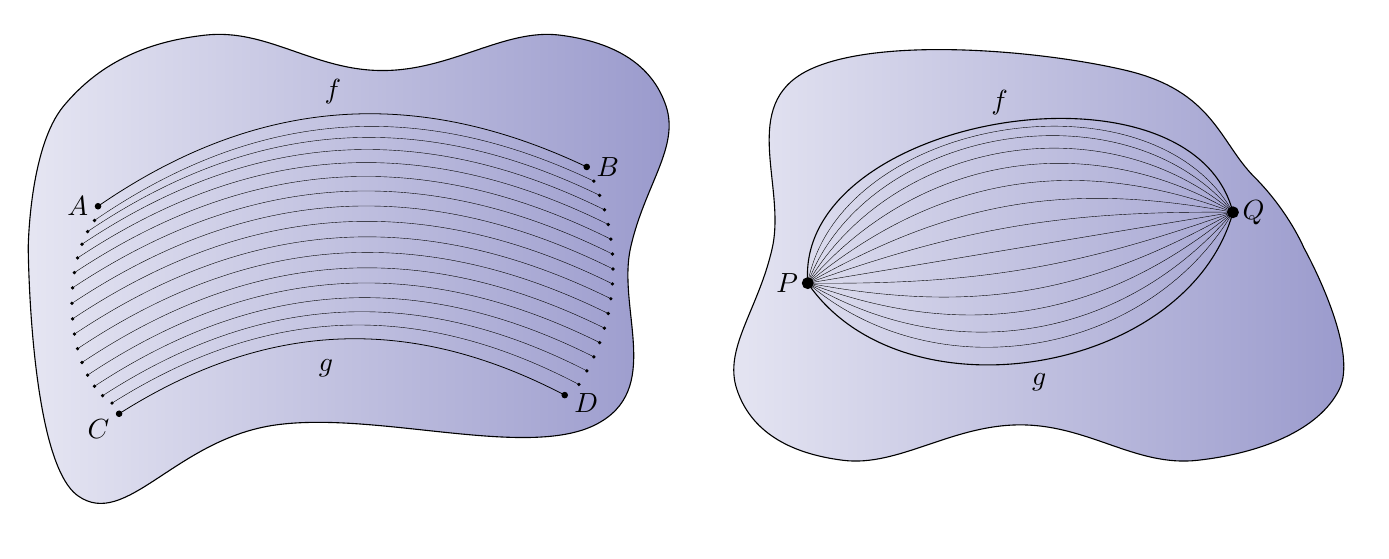
\begin{tikzpicture}[scale = 0.9]
            \begin{scope}
                \shade[draw, left color = NavyBlue!10, right color = NavyBlue!40] 
                plot[smooth, tension=.7] coordinates {(-3.5,0.5)
                (-3,2.5) (-1,3.5) (1.5,3) (4,3.5) (5.5,2.5) (5,.5) (4.5,-2)
                (0,-2) (-2.8,-3) (-3.5,0.5)}; 
        
                \begin{scope}[yshift = 1.2cm]
                    \coordinate (A) at (-2, 0.03);
                    \coordinate (a) at (-2, -3);
        
                    \coordinate (B) at (4, 1);
                    \coordinate (b) at (4, -3);
                    %% establishes the left and right hand coordinates
                    \foreach \t in {4, 5, ..., 18}{
                        \pgfmathsetmacro{\n}{\t*0.05}
                        %% obtains left and right points
                        \path (A) to[bend right = 85] coordinate[pos = \n] (A\t) (a);
                        \path (B) to[bend left = 40] coordinate[pos = \n] (B\t) (b);
                        %% draws circles to mark left and righthand points 
                        \filldraw (A\t) circle (0.1ex);
                        \filldraw (B\t) circle (0.1ex) ;
                        %% draws the lines between the left and right points
                        \draw[line width = 0.05mm] (A\t) to[bend left] (B\t);
                    }
                    %% draws the main top and bottom lines (f  and g)
                    \draw[line width = 0.1mm] ([xshift = 0.1cm,  yshift=-0.15cm]A18) to[bend left] ([xshift = -0.2cm, yshift=-0.15cm]B18);
                    \draw[line width = 0.1mm] ([xshift = 0.05cm,  yshift=0.2cm]A4) to[bend left] ([xshift = -0.1cm, yshift=0.2cm]B4);
    
                    %% draws the circles of the end and start points of the top and bottom lines
                    \filldraw ([xshift = 0.05cm,  yshift=0.2cm]A4) circle (0.25ex) node[left] {$A$};
                    \filldraw ([xshift = -0.1cm, yshift=0.2cm]B4) circle (0.25ex) node[right]{$B$};
                    \filldraw ([xshift = 0.1cm,  yshift=-0.15cm]A18) circle (0.25ex) node[left, yshift=-0.2cm] {$C$};
                    \filldraw ([xshift = -0.2cm, yshift=-0.15cm]B18) circle (0.25ex) node[right, yshift=-0.1cm] {$D$};
                \end{scope}
                %% labels of f and g
                \node at (0.8,2.7) {$f$};
                \node at (0.7,-1.2) {$g$};
            \end{scope}
    
            \begin{scope}[xshift = 12cm, rotate = 180, yshift =-1cm]
                \shade[draw, left color = NavyBlue!10, right color = NavyBlue!40] 
                plot[smooth, tension=.7] coordinates {(-2.5,0.5)
                (-3,2.5) (-1,3.5) (1.5,3) (4,3.5) (5.5,2.5) (5,.5) (4.5,-2)
                (0,-2) (-1.8,-0.5) (-2.5,0.5)}; 
        
                \begin{scope}[xshift = 2.5cm, yshift = 1cm, rotate = 180]
                    \coordinate (A) at (-2, 0);
                    \coordinate (B) at (4, 1);
            
                    \filldraw (A) circle (0.5ex) node[left]{$P$};
                    \filldraw (B) circle (0.5ex) node[right]{$Q$};
            
                    \foreach \p in {0,10,...,50}{
                        \draw[line width = 0.05mm] (A) to[bend right = \p] (B);
                    }
                    \foreach \p in {10,20,...,70}{
                        \draw[line width = 0.05mm] (A) to[bend left = \p] (B);
                    }
                    \draw (A) to[bend left = 85] coordinate (C) (B);
                    \node at ([yshift=0.3cm]C) {$f$};
            
                    \draw (A) to[bend right = 65] coordinate (D) (B);
                    \node at ([yshift=-0.3cm]D) {$g$};
                \end{scope}
            \end{scope}
        \end{tikzpicture}
    \end{center}
    On the above right we have the situation for when $f, g$ start and end at the same point; this homotopy 
    is know as a \textbf{path homotopy}. 
    
    Of course, a homotopy doesn't always exist. When it does, a homotopy can be 
    interpreted as parameterizing, via $t \in [0, 1]$, a family of continuous functions $H_t: X \to Y$
    which \emph{continuously} deform $f$ into $g$\footnote{Caution: a family of continuous functions does not conversely 
    define a homotopy.}. 

    But this story is familar! A natural transformation $\eta: F \to G$ between two functors 
    $F, G: \cc \to \dd$ give rise to a family of morphisms $\eta_A: F(A) \to G(A)$ which are parameterized by  
    the objects of $\cc$ (which also satisfy the naturality property). Below we have this pictured of what this generally looks like. 
    \begin{center}
        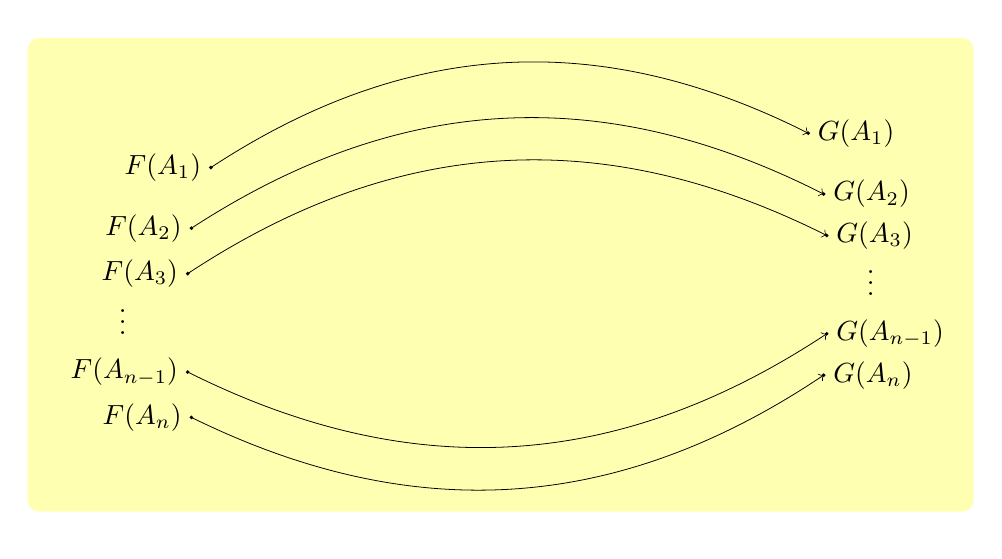
\begin{tikzpicture}
            \filldraw[rounded corners, Yellow!30]
            (-5,-4) rectangle (7, 2);
    
            \begin{scope}[xshift = 0.2cm, yshift=1cm]
                \coordinate (A) at (-2, 0.03);
                \coordinate (a) at (-2, -4);
        
                \coordinate (B) at (4, 1);
                \coordinate (b) at (4, -4);
                %% establishes the left and right hand coordinates
                \foreach \t/\tt in {5/1, 8/2, 10/3}{
                    \pgfmathsetmacro{\n}{\t*0.05}
                    %% obtains left and right points
                    \path (A) to[bend right = 85] coordinate[pos = \n] (A\t) (a);
                    \path (B) to[bend left = 40] coordinate[pos = \n] (B\t) (b);
                    %% draws circles to mark left and righthand points 
                    \filldraw (A\t) circle (0.1ex) node[left]{$F(A_{\tt})$};
                    \filldraw (B\t) circle (0.1ex) node[right]{$G(A_{\tt})$};
                    %% draws the lines between the left and right points
                    \draw[line width = 0.1mm, ->] (A\t) to[bend left] (B\t);
                }
                \node at (-4,-2.5) {$\vdots$}; 
                \node at (5.5,-2) {$\vdots$}; 
                \begin{scope}[yshift=-1.25cm]
                    \coordinate (A) at (-2, 0.03);
                    \coordinate (a) at (-2, -4);
        
                    \coordinate (B) at (4, 1);
                    \coordinate (b) at (4, -4);
                    \foreach \t/\tt in {10/{n-1}, 12/{n}}{
                    \pgfmathsetmacro{\n}{\t*0.05}
                    %% obtains left and right points
                    \path (A) to[bend right = 85] coordinate[pos = \n] (A\t) (a);
                    \path (B) to[bend left = 40] coordinate[pos = \n] (B\t) (b);
                    %% draws circles to mark left and righthand points 
                    \filldraw (A\t) circle (0.1ex) node[left]{$F(A_{\tt})$};
                    \filldraw (B\t) circle (0.1ex) node[right]{$G(A_{\tt})$};
                    %% draws the lines between the left and right points
                    \draw[line width = 0.1mm, ->] (A\t) to[bend right] (B\t);
                }
                \end{scope}
            \end{scope}
        \end{tikzpicture}
    \end{center}
    So, what gives? Is the concept of a natural transformation somewhat logically 
    and conceptually analogous to the concept of a homotopy? The answer is yes, and we can define 
    a natural transformation in the following manner which is strikingly similar to the 
    definition of a homotopy. 
    \begin{definition}\label{definition:nat_trans_homotopy}
        Let $F, G: \cc \to \dd$ be functors. Let $\bm{2}$ be the 
        category with two objects $0, 1$ and a single nontrivial morphism.
        A \textbf{natural transformation} $\eta: F \to G$ is a functor 
        $\eta: \cc \times (\bm{2}) \to \dd$ such that  $\eta(-, 0) = F$
        and $\eta(-, 1)= G$. 
    \end{definition}

    Proving this is left as an exercise.

    {\large \textbf{Exercises}
    \vspace{0.5cm}}
    \begin{itemize}
        \item[\textbf{1.}]
        In what follows, let $F,G: \cc \to \dd$ be a pair of functors.
        Interpret what a natural transformation $\eta: F \to G$ is in each case.  
        \begin{itemize}
            \item[(\emph{i}.)]
            Where $\cc$ is a discrete category, and $\dd$ is arbitrary. Separately, can we have a natural transformation when $\dd$ is discrete?
            \item[(\emph{ii}.)]
            Where $\cc$ and $\dd$ are preorders.

            \item[(\emph{iii}.)] 
            Where $\cc$ and $\dd$ are one-object categories whose morphisms are group. 
            \item[(\emph{iv}.)]
            Where $\cc$ is arbitrary and $\dd$ is $\cat$.
        \end{itemize}

        \item[\textbf{2.}]
        Show that Definition \ref{definition:nat_trans_homotopy} and Definition \ref{definition:nat_trans}
        are equivalent.

        \item[\textbf{3.}]
        Consider the initial discussion of this section. Prove that for two functors 
        $F, G : \cc \to \Set$ such that $F(A) \subset G(A)$ for all $A \in \cc$, 
        the inclusion morphisms $i_A: F(A) \to G(A)$ form a natural transformation 
        $i: F \to G$ if and only if, for each $f: A \to B$ in $\cc$, we have that  
        $F(f) = G(f)|_{F(A)}$. 

        \item[\textbf{4.}]
        Let $\cc$ be a category, and consider two objects $A,B$ 
        so that we  have the functors 
        \[
            \hom_{\cc}(A, -), \hom_{\cc}(B, -): \cc  \to \Set.
        \] 
        \begin{itemize}
            \item[(\emph{i}.)] Let $\phi\in \hom_{\cc}(B,A)$. Show 
            that the family of functions 
            \[
                \phi^*_C: \hom_{\cc}(A,C) \to \hom_{\cc}(B,C)
            \] 
            indexed by each object $C \in \cc$,
            where $\phi^*_C(f: A \to  C) = f \circ \phi: B \to C$,
            forms a natural transformation $\phi^*: \hom_{\cc}(A, -) \to \hom_{\cc}(B, -)$.

            \item[(\emph{ii}.)] Show that every natural transformation 
            $\eta:  \hom_{\cc}(A, -)\to \hom_{\cc}(B, -)$ is constructed 
            in this way. 
        \end{itemize}
        % Let $\bullet: \cc \to \Set$ be the functor where 
        % every object is mapped to $\{\bullet\}$, the one point set, 
        % and every morphism is mapped to its identity morphism. 

        \item[\textbf{5.}]
        Let $F: \cc \to \Set$ be any other functor. Interpret what a 
        natural transformation $\eta: \bullet \to F$ is. 
        What about $\epsilon: F \to \bullet$? 

        \item[\textbf{6.}]
        For every ring $R$ there is a natural inclusion homomorphism $i_R: R \to R[x]$.
        Thus, let $(-)[x]: \ring \to \ring$ be the functor that sends a ring 
        $R$ to its single-variable polynomial ring $R[x]$.
        Show that we have a natural transformation 
        \[
            i: I \to (-)[X]
        \]
        where $I: \ring \to \ring$ is the identity on $\ring$. 

        \item[\textbf{7.}]
        Recall the category of $G$-sets is the category where 
        \begin{description}
            \item[Objects.] All $G$-sets $X$ (i.e., sets $X$ such that $G$ has a 
            group action $\phi:X \times G \to X$)
            \item[Morphisms.] All $G$-equivariant morphisms (i.e., functions $f:X \to Y$
            such that $f(g \cdot x) = g \cdot f(x)$).
        \end{description}
        (Also see Exercise 1.3.6).
        Let $X$ be a $G$-set with action map $\phi: X \times G \to X$ 
        and fix an element $g \in G$. For such an $X$, define the map 
        $\phi_X^g: X \to X$ where $\phi_X^g(x) = \phi(g, x)$. 

        Show that for each $g$, the maps $\phi^g$ form a natural transformation 
        $I \to I$, where $I: \textbf{G}\textbf{-sets} \to \textbf{G}\textbf{-sets}$ 
        is the identity  functor on this category. (Note that this is a nontrivial example of a natural 
        transformation between a functor and itself!)

    \end{itemize}
    

    \newpage
    \section{Monic, Epics, and Isomorphisms}
    In category theory the ultimate focus is placed on the morphisms within a category.
    What we really care about are the relationships between the objects.
    Thus in this section we'll go over \emph{types} of morphisms that exist between objects.

    The way that this is done in set theory is to consider injective functions, surjective 
    functions, and isomorphisms. This can also be done in topology, and in group, ring, and module 
    theory. However, these concepts make no sense in general. This is because
    in general, the morphisms of a category are not functions because in general, 
    the objects of a category are not sets (even if the objects are sets, the morphisms 
    can still be different than functions). 

    We can nevertheless abstract the concept of injections and surjections by 
    expressing their properties categorically; that is, without reference to specific 
    elements in any objects. This leads to the concepts of monomorphisms and epimorphisms.
    \vspace{0.3cm}

    \begin{minipage}{0.8\textwidth}
        \begin{definition}
            Let $f: A \to B$ be a morphism. Then 
            \begin{itemize}
                \item[1.] $f$ is a \textbf{monomorphism} (or is monic) if
                \[ 
                    f \circ g_1 = f \circ g_2 \implies g_1 = g_2
                \]
                for all
                $g_1,g_2 : C \to A$, where $D$ is arbitrary.
                \item[2.] $f$ is a \textbf{epimorphism} (or is epic) if 
                \[ 
                    g_1 \circ f  = g_2 \circ f \implies g_1 = g_2
                \]
                for all $g_1, g_2 : B \to C$, where $C$ is an arbitrary
                object. 
                \item[3.] $f $ is a \textbf{split monomorphism} (or retraction)
                if, for some\\
                $g: B \to A$, 
                \[
                    f  \circ g = 1_B.  
                \]
                \item[4.] $f $ is a \textbf{split epimorphism} (or section) if, for some
                $g: B \to A$, 
                \[
                    g \circ f  = 1_A.
                \]
            \end{itemize}
        \end{definition}
    \end{minipage}
    \hspace{-2cm}
    \begin{minipage}{0.1\textwidth}
        \vspace{-2.2cm}

        \begin{tikzpicture}
            \filldraw[yellow!30, rounded corners]
            (-2.25,-1.5) rectangle (2.25,1.5);
            \node at (0,0){
                \begin{tikzcd}[row sep = 1.2cm, column sep = 1.4cm]
                    C  \arrow[dr,swap, "f \circ g_1 = f \circ g_2"] \arrow[r, yshift=0.7ex, "g_1"] \arrow[r,
                    yshift=-0.7ex,swap,  "g_2"]     
                    &
                    A \arrow[d, "f"]\\
                    & B 
                \end{tikzcd} 
            };
        \end{tikzpicture}
        \vspace{0.2cm}
        
        \begin{tikzpicture}
            \filldraw[yellow!30, rounded corners]
            (-2.25,-1.5) rectangle (2.25,1.5);
            \node at (0,0){
                \begin{tikzcd}[row sep = 1.2cm, column sep = 1.4cm]
                    A \arrow[d, swap, "f"] \arrow[dr, "g_1 \circ f = g_2 \circ f"]\\
                    B \arrow[r, yshift=0.7ex, "g_1"]
                    \arrow[r,yshift=-0.7ex,swap,  "g_2"] & C
                \end{tikzcd}
            };
        \end{tikzpicture}
    \end{minipage}
    \vspace{1cm}

    Monomorphisms and epimorphisms are an abstraction that take advantage key properties 
    of both injective and surjective functions. We illustrate this with a few examples. 

    \begin{example}
        In $\Set$, an injective function $f: X \to Y$ is ``one-to-one'' in 
        the sense that $f(x) = f(y)$ if and only if $x = y$. With that said, suppose that 
        $g_1, g_2: Z \to X$ are functions and moreover that $f\circ g_1 = f \circ g_2$. 
        Then this means that, for all $z \in Z$, we have that 
        \[
            f(g_1(z)) = f(g_2(z)) \implies g_1(z) = g_2(z)    
        \]
        since $f$ is one-to-one. Hence we see that injective functions are 
        monomorphisms in $\Set$; 
        one can then conversely show that a monomorphism in $\Set$ 
        are injective functions. 
    \end{example}

    \begin{example}
        Let $(G, \cdot)$ be a group, and suppose $(H, \cdot)$ is a normal subgroup of 
        $G$. Then with such a construction, we always have access to the 
        inclusion and projection homomorphisms
        \begin{align*}
            i: H \to G \qquad &i(h) = h \\
            \pi: G \to G/H \qquad &\pi(g) = g + H.
        \end{align*}
        It is not hard to see that $i$ is a monomorphism and $\pi$ is an epimorphism; 
        for suppose $\phi, \psi:K \to G$ are two group homomorphisms from some group $K$ 
        where $i \circ \phi = i \circ \psi$. Then for each $k \in K$, $i(\phi(k)) = i(\psi(k))
        \implies \phi(k) = \psi(k)$, so that $\phi = \psi$. Conversely, if $\sigma, \tau: G \to M$ 
        are two group homomorphisms to some group $M$ such that 
        $\sigma \circ \pi = \tau \circ \pi$, then because $\pi$ is surjective we have that 
        $\sigma = \tau$. Hence, we see $\pi$ is an epimorphism.

        Since the above constructions can be repeated in the 
        categories $\ab$, $\ring$, 
        and $R\mod$, so can the above argument. We'll see more generally 
        the deeper reason for why this is the case later on.
    \end{example}


    \begin{example}
        In the category of fields, $\fld$, every nonzero morphism is a 
        monomorphism. This is due to the classic argument: the only nontrivial ideal 
        of a field $k$ its itself; hence the kernal of any map $\phi: k \to k'$ 
        is either trivial or all of $k$. If we suppose $\phi$ is nonzero, then we see 
        that it must be injective, and hence a monomorphism. 
    \end{example}

    \begin{definition}
        Let $f: A \to B$ be a morphism between two objects $A$ and $B$.
        We say that $f$ is an \textbf{isomorphism} if there exists a
        morphism $f^{-1}:B \to A$ in $\cc$! such that 
        \[
            f \circ f^{-1} =\id_A \quad \quad f^{-1} \circ f = \id_B.
        \]
        In this case, $f^{-1}$ is unique, and for any two isomorphisms
        $f:A \to B$ and  $g:B \to C$ we have
        \[
            (g \circ f)^{-1} = f^{-1}\circ g^{-1}.
        \]
        In this case we say that $A$ and $B$ are isomorphic and denote 
        this as $A \cong B$. 
    \end{definition}

    This is a generalization of the familiar concept of isomorphisms
    in abstract algebra and in set theory that one usually encounters. 

    Next, we illustrate a few properties of these types of morphisms.
    \begin{proposition}
        Let $F: \cc \to \dd$ be a functor. Then 
        if $f: A \to B \in \cc$ 
        \begin{itemize}
            \item is an isomorphism, then 
            $F(f)$ is an isomorphism in $\dd$. 
            \item is a split monomorphism, then $F(f)$ 
            is a split monomorphism in $F(f)$  
            \item is a split epimorphism, then $F(f)$ is a split 
            epimorphism.
        \end{itemize}
        That is, functors \textbf{preserve} isomorphisms, split monomorphism, 
        and split epimorphisms. 
    \end{proposition}   
    In general, functors do not \textbf{reflect} isomorphisms, split monomorphisms, 
    and split epimorphisms. That is, if $F(f): F(A) \to F(B)$ is an isomorphism 
    it is not the case that $f$ is an isomorphism.
    
    We demonstrate this with the following example. 

    \begin{example}
        Recall that $\text{Spec}(-): \cring \to \Set$ is a functor 
        that appears in algebraic geometry. It sends every commutative ring $A$ to 
        its ring spectrum $\spec(A)$, which consists of all prime ideals of $A$.

        Let $\displaystyle N =\bigcap_{P \in \spec(A)}P$ be the intersection of all prime ideals.
        An equivalent way to speak of $N$ 
        is the set $N = \{a \in A \mid a^m =0 \text{ for some positive integer }m\}$; 
        that is, $N$ is equivalently the \textbf{nilradical} elements of $A$.

        Now the projection ring homomorphism 
        \[
            \phi: A \to A/N
        \]
        is certainly not an isomorphism (unless $A$ has no nontrivial 
        nilradical elements), but the image of this map under $\spec$ 
        \[
            \spec(\phi): \spec(A/N) \isomarrow \spec(A)
        \] 
        is always an isomorphism. In fact, if we impose the Zarisky topology on these prime spectrums, 
        the functor becomes one which goes to topological spaces
        \[
            \text{Spec}(-): \cring \to \top
        \]
        and the map $\phi$ becomes a homeomorphism. Hence, this functor does not reflect isomorphisms 
        in either the set or topological senses, because the image $\spec(\phi)$ 
        is an isomorphism, but $\phi$ is not.  
        Despite this,  
        the interpretation of this result is a useful one because it demonstrates that algebraic 
        geometrists can ``throw away'' their nilradical elements without changing 
        their Zariski topology.
    \end{example}



    \begin{lemma}\label{lemma:composition_of_epis}
        The composition of monomorphisms (epimorphisms) is a (an) monomorphism
        (epimorphism).
    \end{lemma}

    \begin{prf}
        Let $f: A \to B$ and $g: B \to C$ be
        monomorphisms, and suppose $h_1, h_2 : D \to A$ are two
        parallel morphisms. Suppose that 
        $(g \circ f) \circ h_1 = (g \circ f) \circ h_2.$
        Note that we can rewrite the equation to obtain that 
        \[
            g \circ (f \circ h_1) = g \circ (g \circ h_1) \implies f \circ h_1 = f \circ h_2. 
        \]
        as $g$ is monic, and hence it is left cancellable. 
        But once again, $f$ is monic, so we cancel on the left to
        obtain that $h_1 = h_2$
        as desired.
    \end{prf}

    

    \textcolor{MidnightBlue}{Note: it is not always the case that a
    monic, epic morphism is an isomorphism (that is, it's not always
    invertible.)}

    \begin{example}
        Consider the category $\top$, consisting of (small)
        topological spaces as our objects with continuous functions between
        them as morphisms. Let $D$ be a dense subset of a topological space $X$ and let $i: D
        \to X$ be the inclusion map. We'll show that this function is both
        epic and monic.
    
        To show it is epic, let $f_1, f_2: X \to Y$ be continuous maps
        form $X$ to another topological space $Y$. Let $Y$ be Hausdorff,
        and suppose that 
        \[
            f_1 \circ i = f_2 \circ i.
        \]
        Now $\im(i) = D$, so the above equation tells us that $f_1(d) =
        f_2(d)$ for all $d \in D$. That is, the functions agree on the
        dense subset. However, we know from topology that this implies
        that $f_1 = f_2$.
        \begin{prf}
            \textcolor{MidnightBlue}{
                Suppose that $f_1(x) \ne f_2(x)$ for some $x \notin D$. Since the points are
                distinct, and since $Y$ is Hausdorff, there must exist disjoint open sets 
                $U, V$ in $Y$ such that $f_1(x) \in U$ and $f_2(x) \in V$. Since both $f_1, f_2$ are
                continuous, there must exist open sets $U', V'$ in $X$ such that 
                $f(U') \subset U$ and $g(V') \subset V$. 
                \\
                \indent However, since $D$ is dense in $X$,
                both $U'$ and $V'$ must intersect with some portion of $D$; that is, 
                there is some $y \in U'$ and $z \in V'$ such that $y, z \in D$. Therefore, 
                we see that $f_1(y) \in U$ and $f_2(z) \in V$, and since
                $y, z \in D$ we have that $f_1(y) = f_2(z)$. But this contradicts the fact that $U \cap V =
                \emptyset.$ Therefore, we have a contradiction and it must be the case that 
                $f_1(x) = f_2(x)$ for all $x \in X$, as desired.
            }
        \end{prf}
        \noindent Therefore, we see that $i$ is epic. To show that it is
        monic, suppose $g_1, g_2: Y \to D$ are two 
        parallel, continuous functions, and that 
        \[
            i \circ g_1 = i \circ g_2.
        \]
        Since $i$ is nothing more than an inclusion map, we immediately
        have that $g_1 = g_2$. Therefore, $i$ is also monic.
    
        \textbf{However}, note that $i: D \to X$ is not an isomorphism, since 
        it is not necesasrily always surjective.
        Hence $i$ is an example
        of a monic, epic morphism which is not an isomorphism. 
        
    \end{example} 

    We finish our discussion on monics and epics by considerig the automorphism groups 
    of a category. 

    \begin{definition}
        Let $\cc$ be a locally small category. For each object $A$ in $\cc$, we can consider the 
        \textbf{automorphism group} $\aut(A)$ whose objects consist of isomorphisms 
        $\phi: A \isomarrow A$, whose product is composition, and whose identity is $1_A$. 
    \end{definition}

    Note that despite the notation, this does \emph{not} generally define a functor. 

    \begin{example}
        Some examples of the above construction include familiar and useful examples 
        in mathematics.
        \begin{itemize}[itemsep=0.5cm]
            \item  For any group $(G, \cdot)$ in $\grp$, we can formulate the automorphism 
            group $\aut(G)$ which is the group of isomorphisms from $G$ to itself. 
            Depending on $G$, this can have all kinds of behavior. For example, if 
            $\aut(G)$ is cyclic, then 
            $G$ is abelian. If $G$ is an abelian group 
            of order $p^n$, then $\aut(G) = GL(n, F)$ where $F$ is the finite field of order $p$.
    
            \item For any set $X$ in $\Set$, the automorphism group $\aut(X)$ consists of the bijections 
            on $X$ to itself; by definition in set theory, these are just permutations. Hence the automorphism group 
            is the permutation group of the elements of $X$. 
    
            \item For any field $(k, \cdot, +)$ in $\fld$, the automorphism 
            group $\aut(k)$ also consists of field isomorphisms to itself. 
            In this setting, what is often 
            of more interest is considering the subgroups of $\aut(k)$, often 
            denoted as $\aut(k/L)$, which are automorphisms that fix the subfield 
            $L$. These subgroups are key 
            to studying polynomial roots and hence are prevalent in Galois theory.
    
            \item For any graph $(G, E, V)$ in \textbf{Grph}, one can construct the automorphism group $\aut(G)$, 
            which tracks the symmetries of the graph. Interestingly, there is a theorem known as 
            Frucht's Theorem which states that every finite 
            group is the automorphism group of a finite (undirected) graph; this was later 
            extended and shown that every group is the automorphism group of a directed 
            graph [\emph{Groups represented by homeomorphism groups}.]. 
    
            \item For any topological space $(X, \tau)$ in $\top$, 
            the autormorphism group $\aut(X)$ 
            consists of the homeomorphisms to itself. Geometrically, these record the possible 
            ways of continuously deforming a space back into itself. It is a theorem 
            that every group is the automorphism group of some complete, connected, 
            locally connected metric space $M$ of any dimension.         
        \end{itemize}
    \end{example}


    With the automorphism group in mind, we might ask the same question on the object 
    level:
    Given an object $A$ in $\cc$, what objects are isomorphic to $A$ in $\cc$?
    To answer this, we define the relation 
    $\sim$ on $\ob(\cc)$, the objects of $\cc$, where we say 
    \[
        A \sim B \text{ if } A \cong B.
    \]  
    Such an equivalence relation divides the objects of $\cc$ into disjoint 
    \emph{isomorphsm classes}, which reduces the structure of $\cc$. 

    \begin{definition}
        Let $\cc$ be a category and $A$ any object. We call the equivalence class 
        of $A$ under $\sim$, defined previously, as the \textbf{isomorphism class} 
        which we denote as 
        \[
            \text{Isom}(A) = \{X \in \ob(\cc) \mid X \cong A\}.
        \]
    \end{definition}

    This leads to the following categorical construction which preserves a great 
    deal of information within the category.

    \begin{definition}
        Let $\cc$ be a category, and assume the axiom of choice. Then we can construct 
        \textbf{a skeleton of a category $\cc$}, denoted $\text{sk}(\cc)$, as 
        the category where 
        \begin{description}
            \item[Objects.] For each $A \in \cc$, we select one 
            representative of each isomorphism class $\text{Isom}(A)$.
            \item[Morphisms.] For two representatives of isomorphism 
            classes $A, B$, we take 
            \[
                \hom_{\text{sk}(\cc)}(A,B)= \hom_{\cc}(A,B)
            \] 
        \end{description}
    \end{definition}
    We note three things regarding this construction. 
    \begin{description}
        \item[(1)] We used the axiom of choice to build the objects of the 
        category, since we needed to select one element from each isomorphism class.
        \item[(2)] The category $\text{sk}(\cc)$ is a full subcategory of $\cc$ by definition.
        \item[(3)] We note that this construction builds \emph{a} skeleton. In general, 
        a category will have different skeletons because there are many ways to construct the 
        objects of such a skeleton. 
    \end{description}
    As noted, a category will have different skeletons. However, up to isomorphism, it does 
    not really matter which skeleton we build as we will see. 
    
    \begin{lemma}\label{lemma:skeletons_are_isomorphic}
        Let $\cc$ be a category, and let $\text{sk}(\cc)$ and $\text{sk}'(\cc)$ 
        be two skeletons built from $\cc$. Then $\text{sk}(\cc) \cong \text{sk}'(\cc)$. 
    \end{lemma}

    The prove is left as an exercise for the reader. We will see late that there 
    are more enjoyable properties of ``skeletal'' categories, which we define as categories 
    exhibiting this type of behavior.

    \begin{definition}
        A category $\cc$ is called \textbf{skeletal} if no two distinct objects are isomorphic in $\cc$.
    \end{definition}

    Categorical skeletons are inadvertently studied everywhere in mathematics. 
    For example, asking for a classification of abelian groups, of manifolds, or 
    even of the cardinality of every set is the same thing as asking for the 
    skeletons of $\ab$, $\textbf{DMan}$, and $\Set$. We give a few 
    examples. 

    \begin{example}
        Consider the category $\textbf{FinCard}$ (read: ``finite cardinals'') which we describe as 
        \begin{description}
            \item[Objects.] The set $\varnothing$ and the sets $\{1, 2, ..., n\}$ for each $n \in \mathbb{N}$.
            \item[Morphisms.] All functions between these finite sets.  
        \end{description}
        Clearly this is a full subcategory of $\finset$. Moreover, it is skeletal; 
        no two sets are isomorphic because each object is of different size. Therefore, it 
        is skeletal. In fact, $\textbf{FinCard}$ is a skeleton 
        of $\finset$ because any finite set (in some universe $U$) 
        can be ordered in some way, which provides an enumeration on its objects.
        In other words, every finite set is of some finite size, making it isomorphic 
        to some set $\{0, 1, 2, \dots, n\}$. 
    \end{example}

    \begin{example}
        One can try to generalize the previous example to $\Set$, but this 
        is in general not possible unless we assume ZFC with the 
        \textbf{generalized continuum hypothesis}, as such a posulate is independent of ZFC. 
        
        Assuming such an axiom, we can construct the category $\textbf{Card}$
        where 
        \begin{description}
            \item[Objects.] The sets $\varnothing, \{1, 2, \dots, n\}$ for each $n \in \mathbb{N}$, and $\omega_0, \omega_1, \omega_2, \dots$ 
            \item[Morphisms.] All functions between such sets. 
        \end{description}
        Here we see that this is again a skeleton $\Set$, since by our assumptions 
        (which is assuming a lot), any set is of some cardinality
        $1, 2, \dots, n, \dots, \aleph_0, \aleph_1, \dots$. However, for each such 
        cardinal we have a corresponding set with that cardinality. Hence each element 
        in $\Set$ is isomorphic to some element of $\textbf{Card}$. Overall, 
        we see that \textbf{Card} forms a skeleton of $\Set$.
    \end{example}

    The above example can be repeated for \textbf{Cycl}, the category of cyclic groups.
    This is because any two cyclic groups of the same order are isomorphic. Hence, one 
    can find a skeleton of \textbf{Cycl} by finding a family of cylic groups of every set 
    size (again, using the generalized continuum hypothesis).  

    \begin{example}
        Consider the category $\textbf{Ecld}$ of Euclidean spaces, which we may
        describe as 
        \begin{description}
            \item[Objects.] The vector spaces $\rr^n$ for each $n = 0, 1, 2, \dots, $
            \item[Morphisms.] Linear transformations between vector spaces. 
        \end{description}
        Then we see that $\textbf{Ecld}$ is the skeleton of $\textbf{FinVect}_k$, 
        which is the category of finite-dimensional vector spaces. The reason why this 
        works is because every finite dimensional vector space is isomorphic to $\rr^n$ for 
        some $n$. 
    \end{example}

    {\large \textbf{Exercises}
    \vspace{0.5cm}}
    \begin{itemize}
        \item[\textbf{1.}] Prove Lemma \ref{lemma:composition_of_epis} for epimorphisms.

        \item[\textbf{2.}] Prove Lemma \ref{lemma:skeletons_are_isomorphic}.
        \item[\textbf{3.}] Describe the monomorphisms and epimorphisms 
        in the category of $\cat$.\footnote{Classifying epimorphisms 
        in $\cat$ is actually nontrivial, although not impossible. 
        However, the task here is to just interpret 
        the definition of monics and epics $\cat$. }

        \item[\textbf{4.}]
        In the category of $\ring$, give an example of a morphism 
        which is both a monomorphism and epimorphism, but not an isomorphism.
        \\
        (\emph{Hint:} Consider the inclusion $i: \zz \to \qq$.)

        \item[\textbf{5.}]
        Recall from Exercise ? that, in any category, if we have two commutative 
        diagrams, we can always stack them together to obtain a larger commutative diagram. 
        We saw, however, that converse is not always true: subdividing a commutative 
        diagram does not produce smaller commutative diagrams. 
        
        Prove that the converse is true when all morphisms are isomorphisms.     
    \end{itemize}


    % For any category $\cc$, we have three forgetful functors 
    % \begin{gather*}
    %     F_{mon}: \cat \to \cat_m\\
    %     F_{epi}: \cat \to \cat_e\\
    %     F_{iso}: \cat \to \textbf{Grpd}
    % \end{gather*}
    % where $\cat_m$ consists of categories whose morphisms are 
    % monomorphisms, $\cat_e$ consist of categories whose morphisms are 
    % epimorphisms, and $\textbf{Grpd}$ is the category of groupoids, which equivalently 
    % consists of categories whose morphisms are all isomorphisms. We will see later 
    % that these are part of something we call an ``adjunction,'' which 
    % will be defined later. 



    \newpage
    \section{Initial, Terminal, and Zero Objects}
    We can also be more specific in discussing the nature of the
    objects of a given category $\cc$.

    \begin{definition} 
        Let the following objects exist in some category $\cc$. 
        \begin{itemize}
            \item Let $T$ be an object. Then $T$
            is \textbf{terminal} if for each object $A$, there
            exists exactly one morphism $f_A$ such that $f_A:
            A \to T$. 

            \item Let $I$ be an object. Then $I$ is said to be
            \textbf{initial} if for each object $A$ there exists
            exactly one 
            morphism $f_A : I \to A$. 

            \item An object $Z$ is said to be a \textbf{zero object}
            if it is both terminal and initial. Since terminal and initial objects 
            are unique, so is a zero object.
            
            Equivalently, it is
            zero if for any objects $A, B$, there exists exactly one
            morphism $f: A \to Z$ and exactly one morphism $g: Z  \to
            B$. Hence, for any two objects there exists a morphism between them,
            namely given by
            by $g \circ f$, called the \textbf{zero morphism} from $A$ 
            to $B$. 
        \end{itemize}
        If an object $T$ is terminal, then there is one and only
        morphism to itself (namely, its identity). Therefore,
        for any two terminal objects $T$ and $T'$, they are
        isomorphic, since by assumption there exists unique morphisms
        $f: T \to T'$ and $g: T' \to T$ and we have no choice but to
        say 
        \[
            f \circ g = 1_T \quad g \circ f = 1_{T'}.
        \]
    \end{definition}

    \begin{example}
        Recall that in the category $\grp$, there exists a trivial group 
        $\{e\}$. Moreover, for each group $G$, there exist unique group homomorphisms 
        \[
            i_G: \{e\} \to G \qquad e \mapsto e_G 
        \]
        and 
        \[
            t_G: G \to \{e\} \qquad g \mapsto e_G.
        \]
        Note that both are group homomorphisms since they both behave on identity elements 
        and are trivially distributive across group operations. This then shows that 
        $\grp$, the trivial group is initial and terminal and hence a zero object. 

        This makes sense since for any two groups $G, H$, there exists a unique map 
        \[
            z: G \to H \qquad g \mapsto e_H
        \]
        which could be factorized as 
        \begin{center}
            \begin{tikzcd}[row sep = 1.2cm, column sep = 1.4cm]
                &
                \{e\}
                \arrow[dr, "i_H"]
                &
                \\
                G \arrow[rr, swap, "z"]
                \arrow[ur, "t_G"]
                &
                &
                H
            \end{tikzcd}
        \end{center}
        which demonstrates the existence of a zero object (the name "zero" makes sense now, right?), 
        which we already know is $\{e\}$.
        Note in this example, we did not actually use much group theory. In fact, this could be repeated 
        for the categories $R\mod$, $\ab$, and other similar categories. 
    \end{example}

    The next two examples demonstrate that terminal and initial objects of course don't 
    always have to coincide like they did in the previous example. 

    \begin{example}
        Let $n$ be a positive integer. Recall that we can create a category, specifically a 
        preorder, by taking our objects to be positive integers less than $n$, 
        and allowing one morphism $f: k \to m$ whenever $k \le m$.
        \begin{center}
            \begin{tikzcd}
                1 \arrow[r] \arrow[out=120,in=60,looseness=3,loop]
                &
                2 \arrow[r] \arrow[out=120,in=60,looseness=3,loop]
                &
                3 \arrow[r] \arrow[out=120,in=60,looseness=3,loop]
                &
                \cdots \arrow[r] 
                & 
                n \arrow[scale = 2.5, out=123,in=57,looseness = 3, loop]
            \end{tikzcd}
        \end{center}
        Then 1 is an initial object while $n$ is a terminal object. This 
        is because for any number $1 \le m \le n$, there exists a unique morphism 
        from $1$ to $m$, and a unique morphism $m$ to $n$, both which may 
        be obtained by repeated composition. 
    \end{example}

    \begin{example}
        Consider the category $\Set$. Let $X$ be a given set in this category. 
        Then there are two unique functions which we may construct. First, there is the function 
        \[
            t_X: X \to \{\bullet\}
        \]
        where everything in $X$ is mapped to the one element $\bullet$ of the one point set. 
        Secondly, we may construct a function whose domain is the empty set, 
        and whose codomain is $X$, as below.
        \[
            i_X: \varnothing \to X
        \]
        Thus we have that, in $\Set$, the one point set is a terminal 
        object $\{\bullet\}$ while the empty set
        $\varnothing$ is an initial object.
        
        One may wonder at this point: How exactly is $i_X$ a true, set theoretic function?
        And why can't we also obtain a unique morphism $i'_X: X \to \varnothing$, 
        so that $\varnothing$ is a terminal object as well?

        The second question is easy to answer; if $\varnothing$ was also terminal, then 
        we'd have that $\{\bullet\} \cong \varnothing$ which is not true. Since this is a bit of a boring 
        answer, we'll explain in detail.
        
        Recall that a function in $f: A \to X$ between two sets $A$ and 
        $X$ is a relation $R \subset A \times X$ which satisfies two properties. 
        \begin{itemize}
            \item[1.] (Existence.) For each $a \in A$, there exists a
            $x \in X$ such that $(a, x) \in R$ 
            \item[2.] (Uniqueness. Or, if you'd like, the vertical line test.) 
            If $(a, x) \in R$ and $(a, x') \in R$ then $x = x'$. 
        \end{itemize}
        Now observe that if $A = \varnothing$, then $R \subset \varnothing \times X = \varnothing$. 
        Hence (1) and (2) are satisfied because each is trivially true. However, we don't get 
        a function $f: X \to \varnothing$, since in this case (1) fails. Specifically, (1) demands 
        the existence of elements in our codomain, a demand we cannot meet if it is empty. 
        
        Thus we see that $\varnothing$ is initial, but not terminal as our intuition may suggest, 
        and that $\{\bullet\}$ is terminal.
    \end{example}

    \begin{example}
        Consider the category of fields $\fld$. Suppose we ask if this has an initial 
        or terminal object. 

        We might guess that the smallest field 
        \[
            \mathbb{F}_2 \cong (\zz/2\zz, +, \cdot) = \{0, 1\} 
        \]
        which has characteristic 2 is an initial object. However, this fails to be initial. 
        Observe that the only homomorphism between $\mathbb{F}_2$ and $\mathbb{F}_3$ is the zero 
        homomorphism, which is not in our category. (Recall that $\fld$ is a full subcategory 
        of $\ring$, a category whose morphisms we require to be unit preserving.)
        
        The reason why it must be the zero homomorphisms is because $\mathbb{F}_3$ has characteristic three, 
        and in general, two fields will only share a (nonzero) field homomorphisms if they 
        have the same characteristic. 

        By a similar argument, we can state that terminal objects also do no exist. Overall, 
        these objects fail to exist in $\fld$ because fields have a large set of 
        restictions imposed by their numerous axioms.
        Hence, this category lacks initial and terminal objects.
    \end{example}

    {\large \textbf{Exercises}
    \vspace{0.5cm}} 
    \begin{itemize}
        \item[\textbf{1.}] 
        \begin{itemize}
            \item[(\emph{i}.)] Let $\cc$ be a category with initial object $I$. 
            For any two objects $A, B \in \cc$, define for each $f \in \hom_{\cc}(A, B)$
            the functor
            \[
                P_f: \textbf{2} \to \cc
            \] 
            such that $P(\textcolor{NavyBlue}{\bullet}) = A$, $P(\textcolor{Orange}{\bullet}) = B$, 
            and $P_f(\textcolor{NavyBlue}{\bullet} \to \textcolor{Orange}{\bullet}) = f: A \to B$. 
            Show that for each $f: A \to B$ in $\cc$, we have a natural transformation 
            \[
                \eta: P_{1_I} \to P_f.
            \]
            Note that $1_I: I \to I$ is the identity on the initial object.
            \item[(\emph{ii}.)]
            Suppose we don't know if $\cc$ has an initial object, 
            but we have a distinguished object 
            $I'$ with the property that for each $f \in \hom_{\cc}(A,B)$ there is a natural 
            transformation 
            \[
                \eta: P_{1_{I'}} \to P_f.
            \]
            Is $I'$ an inital object?

            \item[(\emph{iii}.)] Dualize your work for terminal objects.\\
            (\emph{Hint}: We now want a natural transformation $\eta': P_f \to P_{1_I})$.  
        \end{itemize}

    \end{itemize}

    